\documentclass[a4paper,12pt]{article}
\usepackage{graphicx}

\begin{document}

\title{Syncloud - Setup manual}
\date{\today}

\maketitle

\begin{figure}[htbp!]
	\centering
	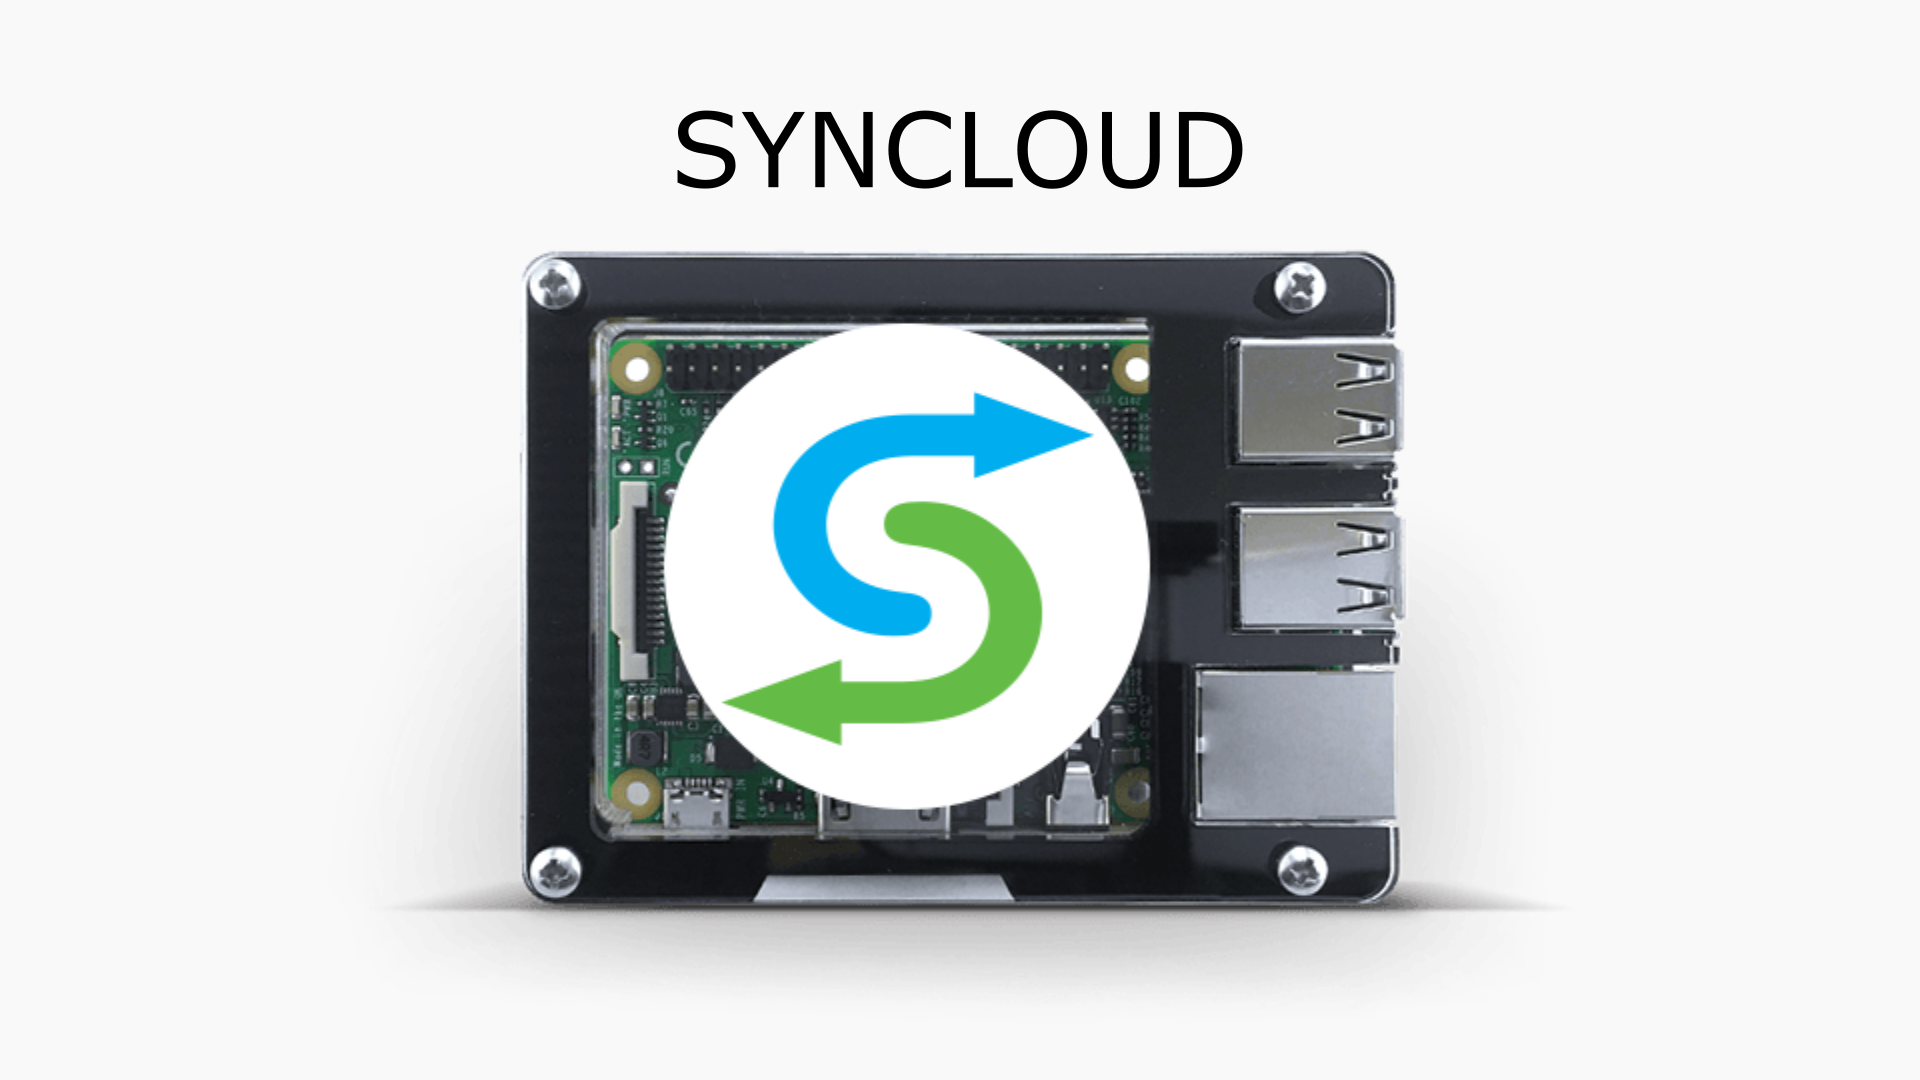
\includegraphics[width=0.7\linewidth]{../frames/1.png}
\end{figure}

\pagebreak

\section{Hallo World}

\begin{figure}[htbp!]
	\centering
	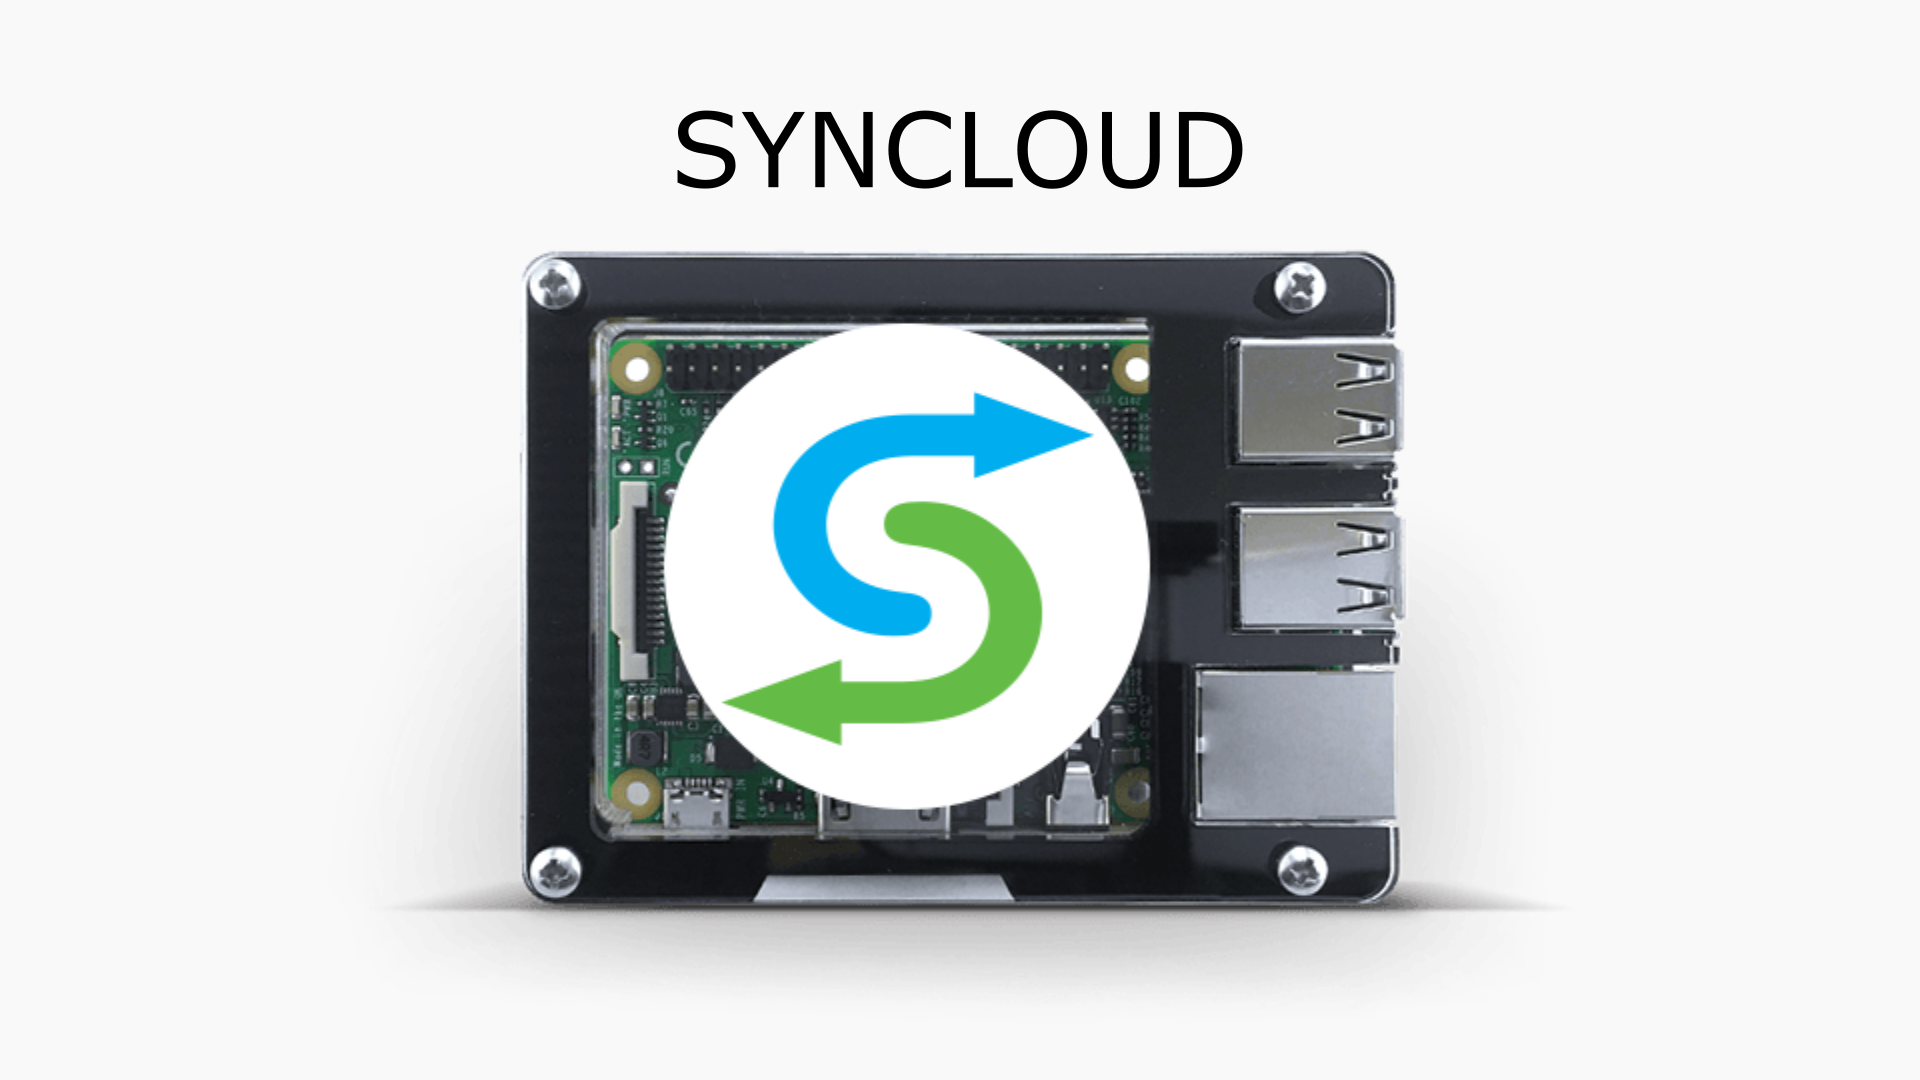
\includegraphics[width=0.7\linewidth]{../frames/1.png}
	\caption{Hello world,
		This is Syncloud and I will show you how to setup your device.}
	\label{fig:1}
\end{figure}

\begin{figure}[htbp!]
	\centering
	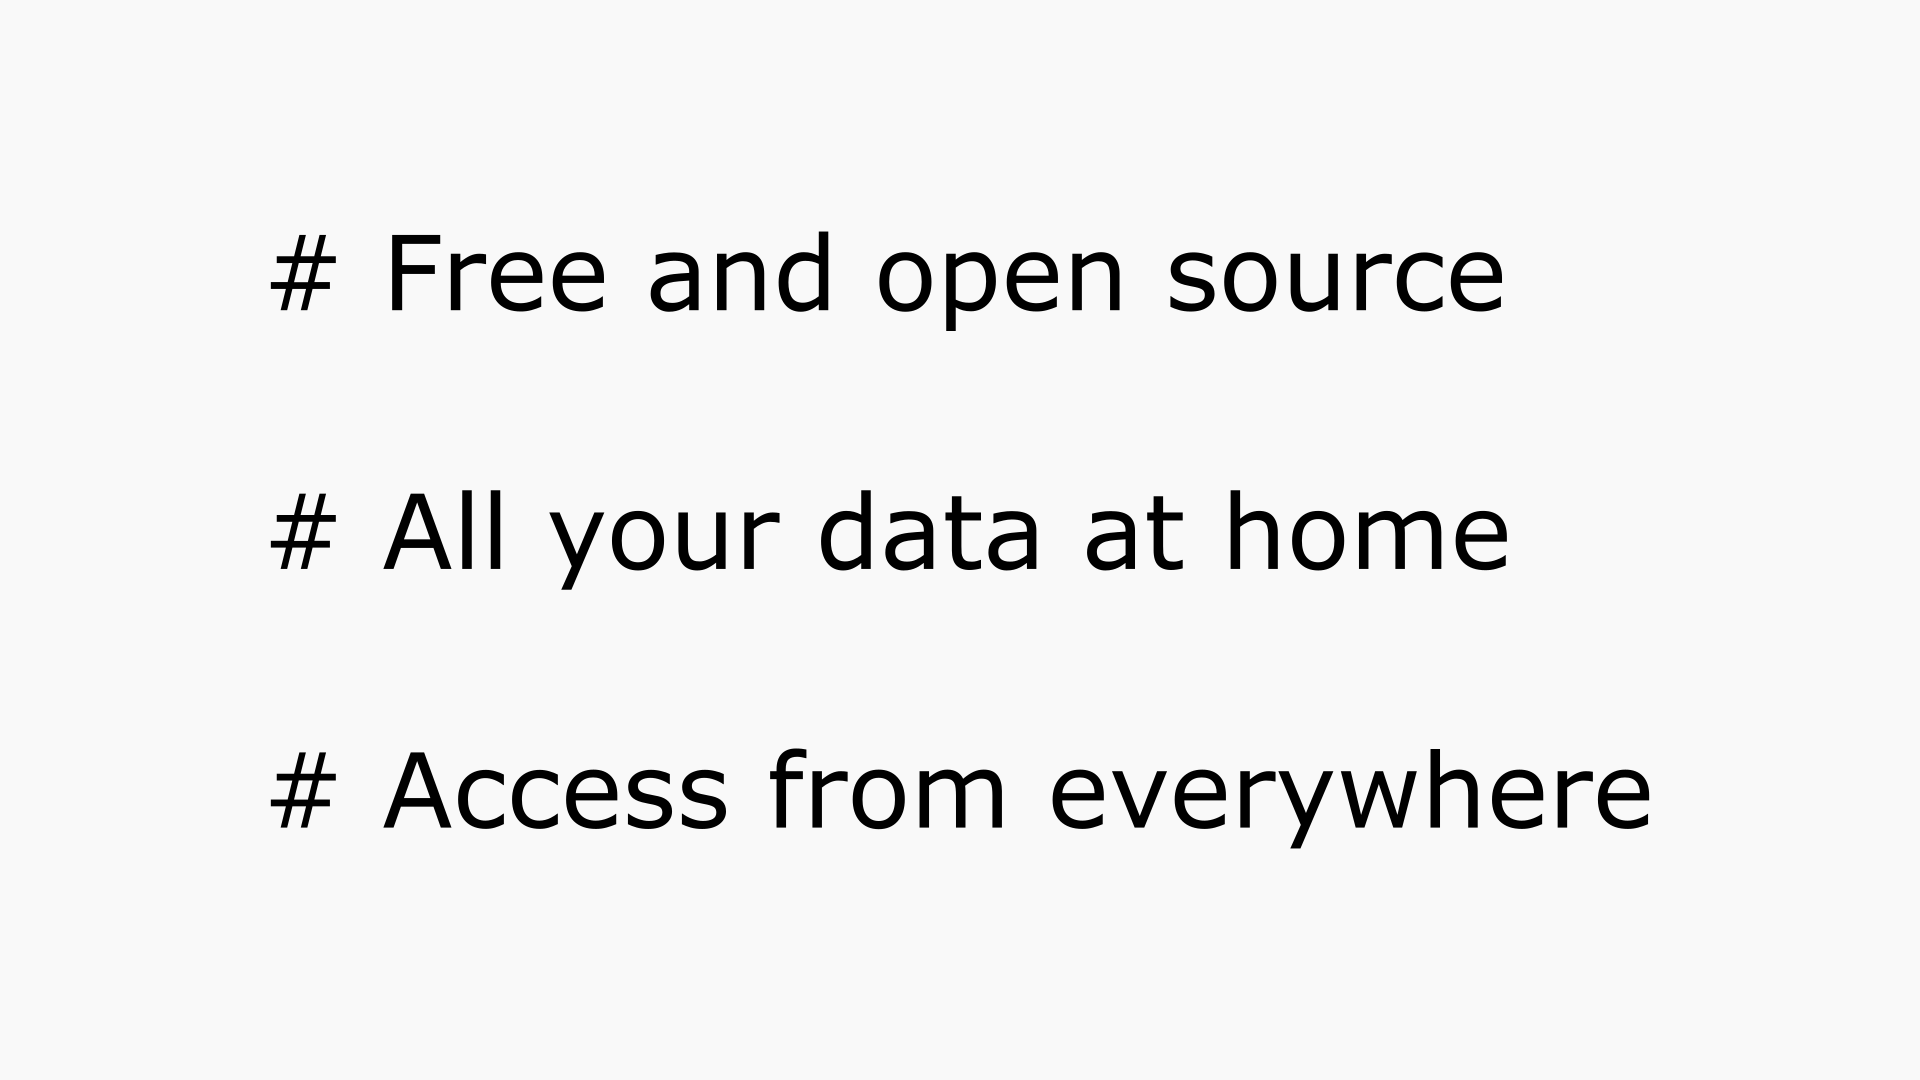
\includegraphics[width=0.7\linewidth]{../frames/2.png}
	\caption{Syncloud is free and open source. All your data will be stored at home, which you can easily access from all over the world.}
	\label{fig:2}
\end{figure}

\section{Get Hardware}

\begin{figure}[htbp!]
	\centering
	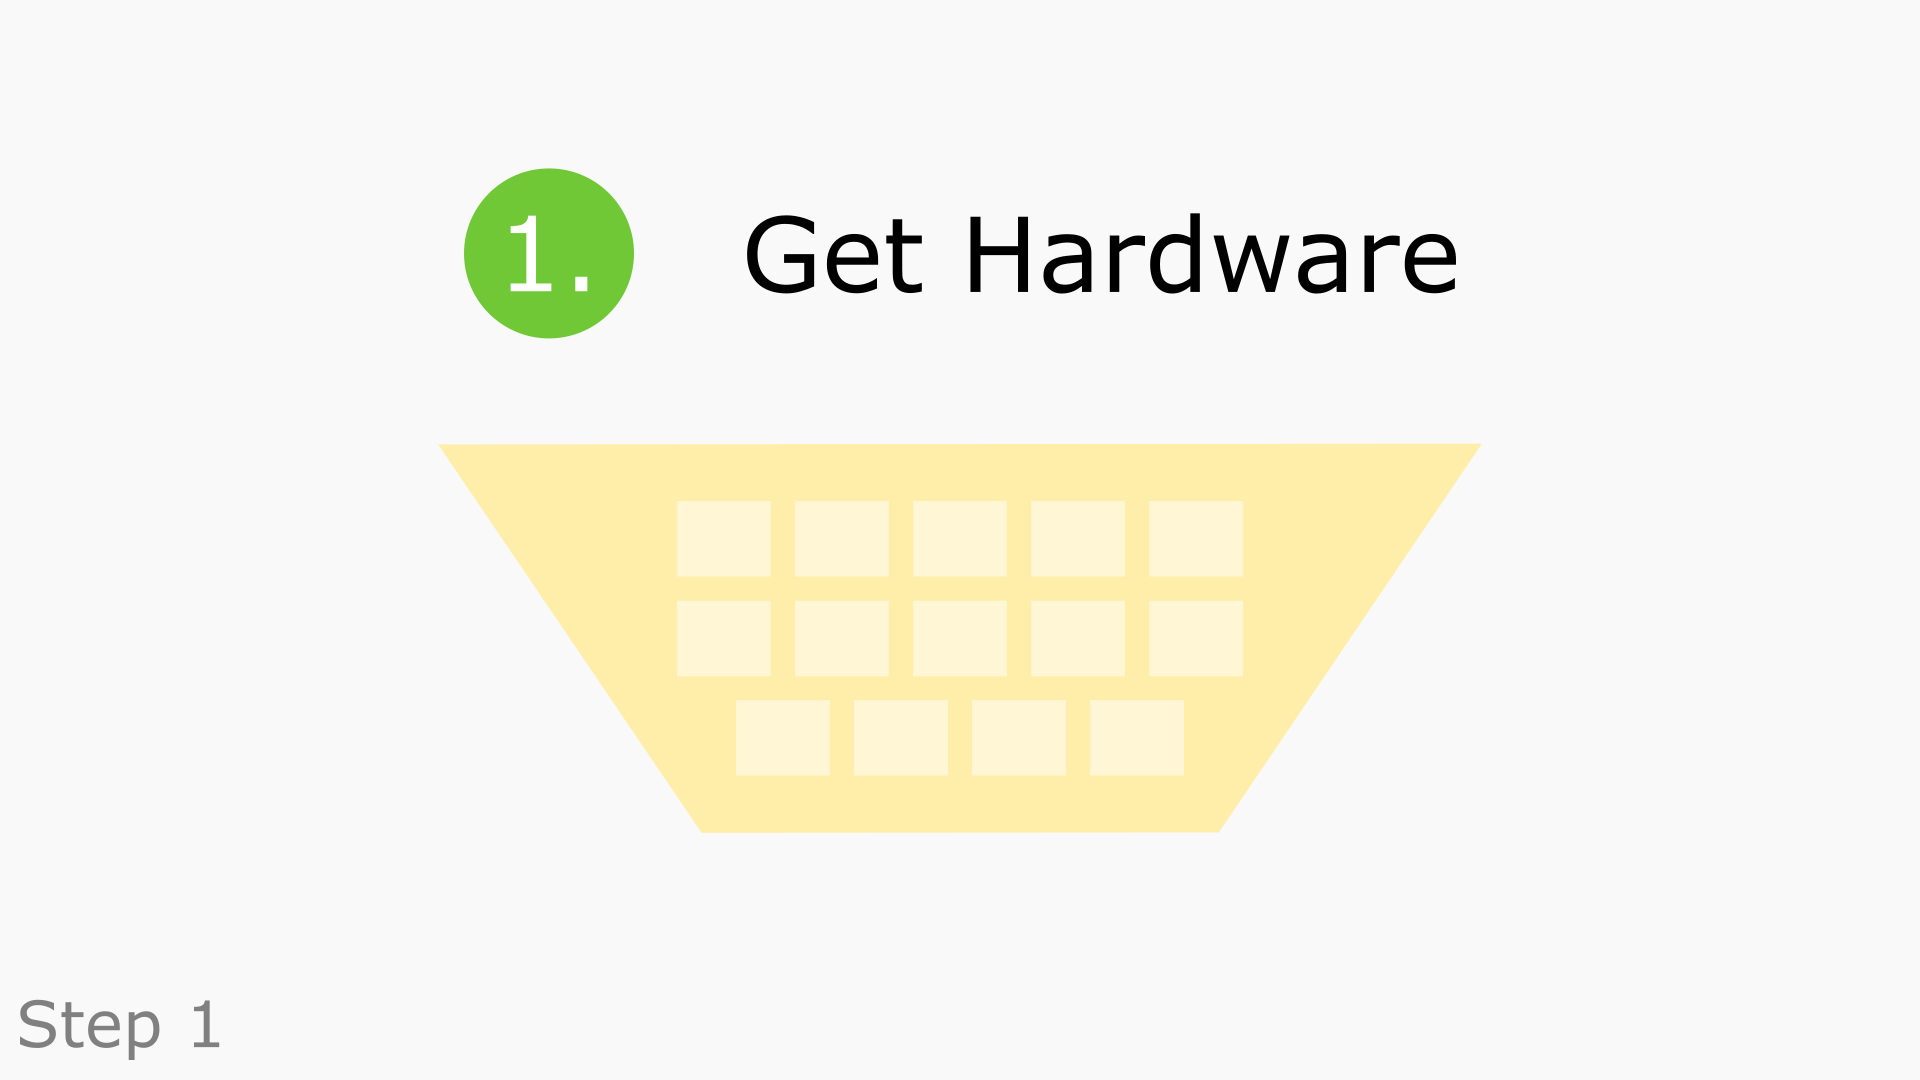
\includegraphics[width=0.7\linewidth]{../frames/3.png}
	\caption{First, it’s time to get a Syncloud device.}
	\label{fig:3}
\end{figure}

\begin{figure}[htbp!]
	\centering
	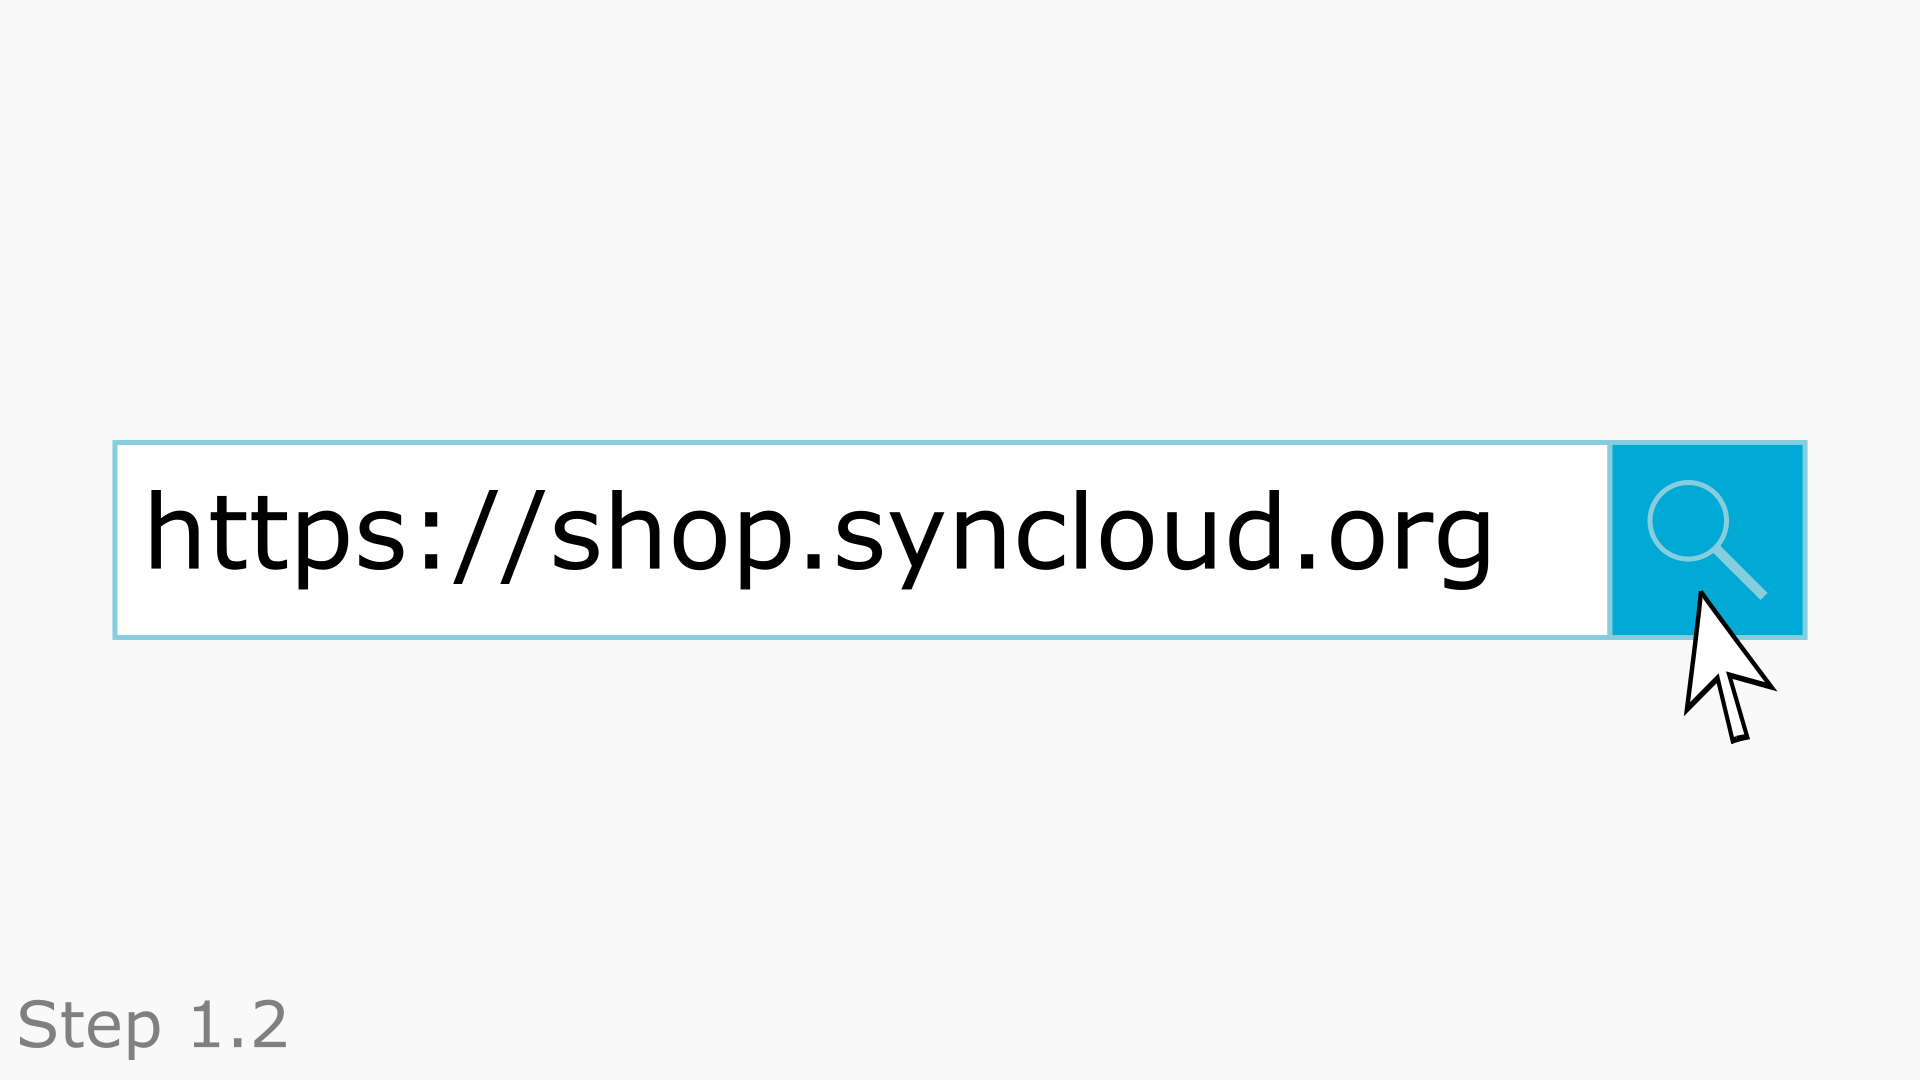
\includegraphics[width=0.7\linewidth]{../frames/13.png}
	\caption{You can buy a plug-and-play device in our shop. You can find our shop under shop dot syncloud dot org.}
	\label{fig:4}
\end{figure}

\begin{figure}[htbp!]
	\centering
	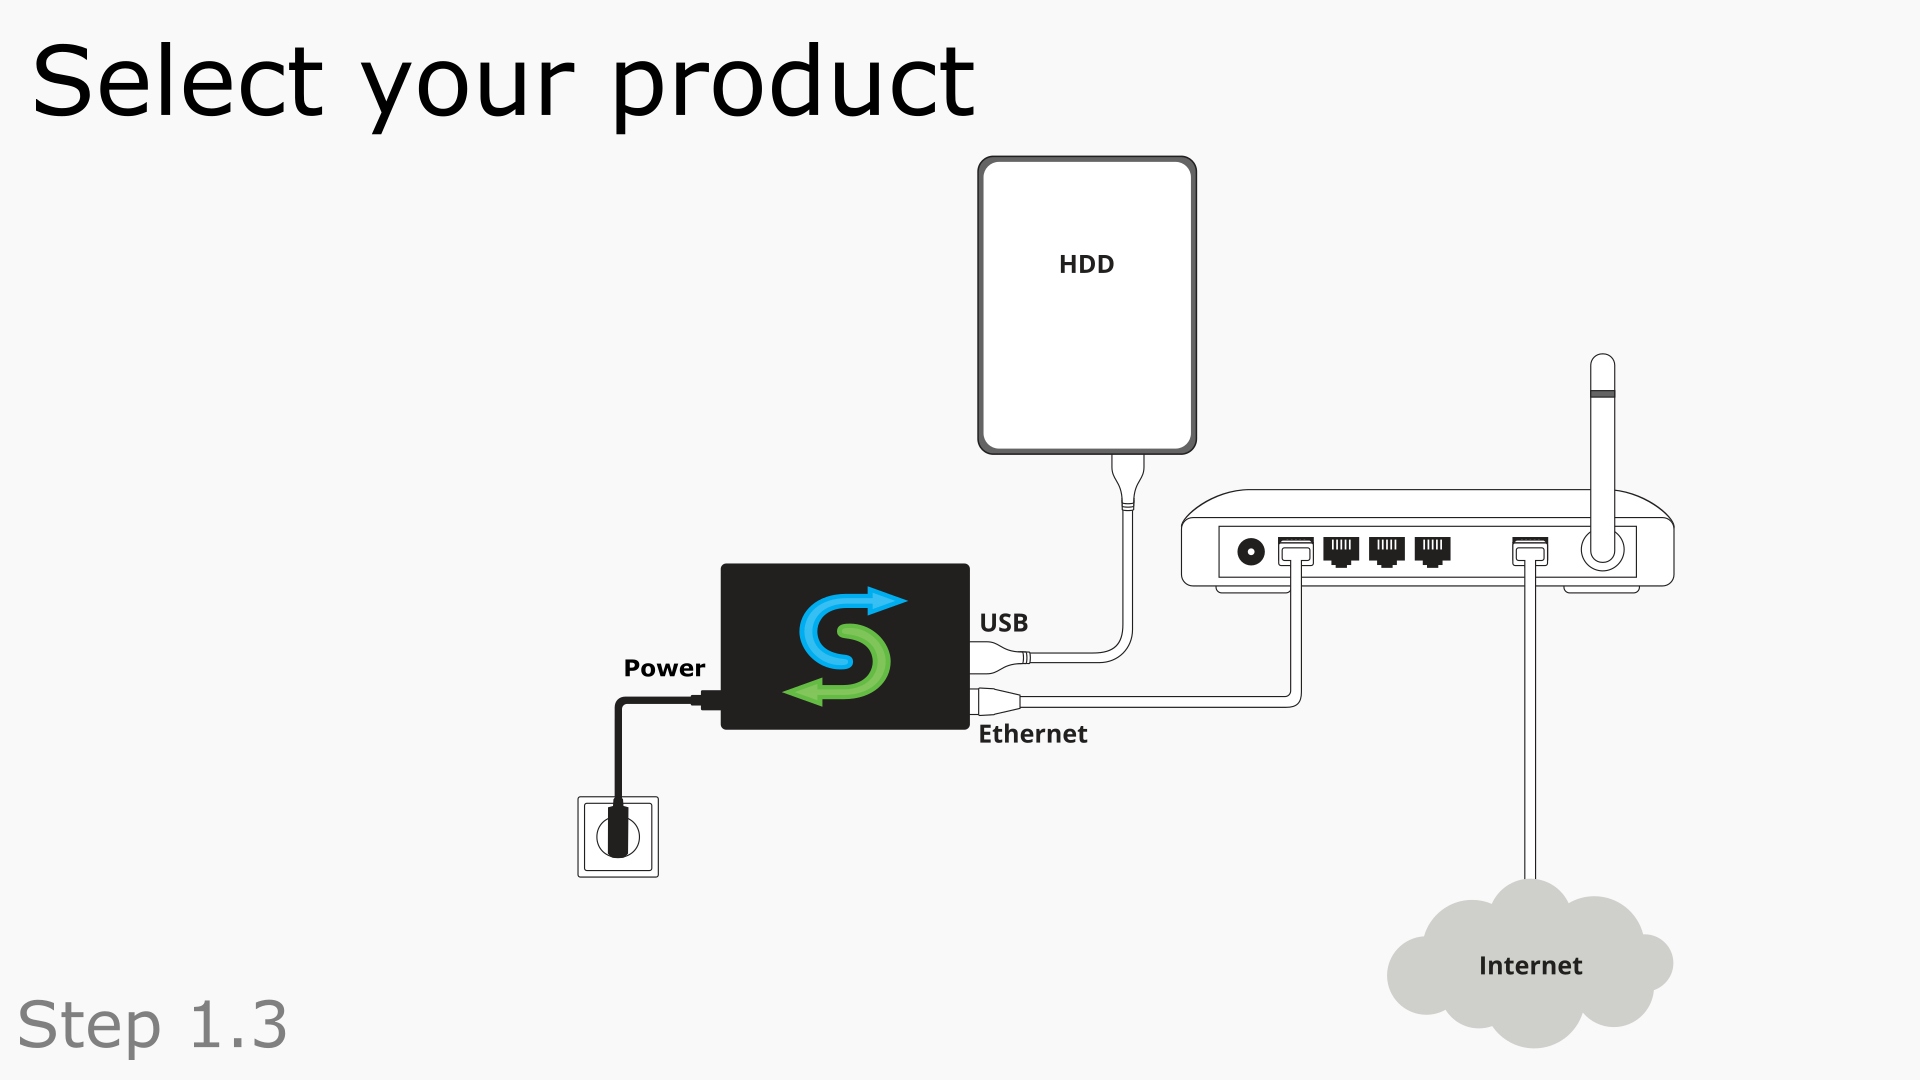
\includegraphics[width=0.7\linewidth]{../frames/14.png}
	\caption{Later, you must connect your device to your router and depending on the device type, to an external storage, as well. We offer two types of devices.}
	\label{fig:5}
\end{figure}

\begin{figure}[htbp!]
	\centering
	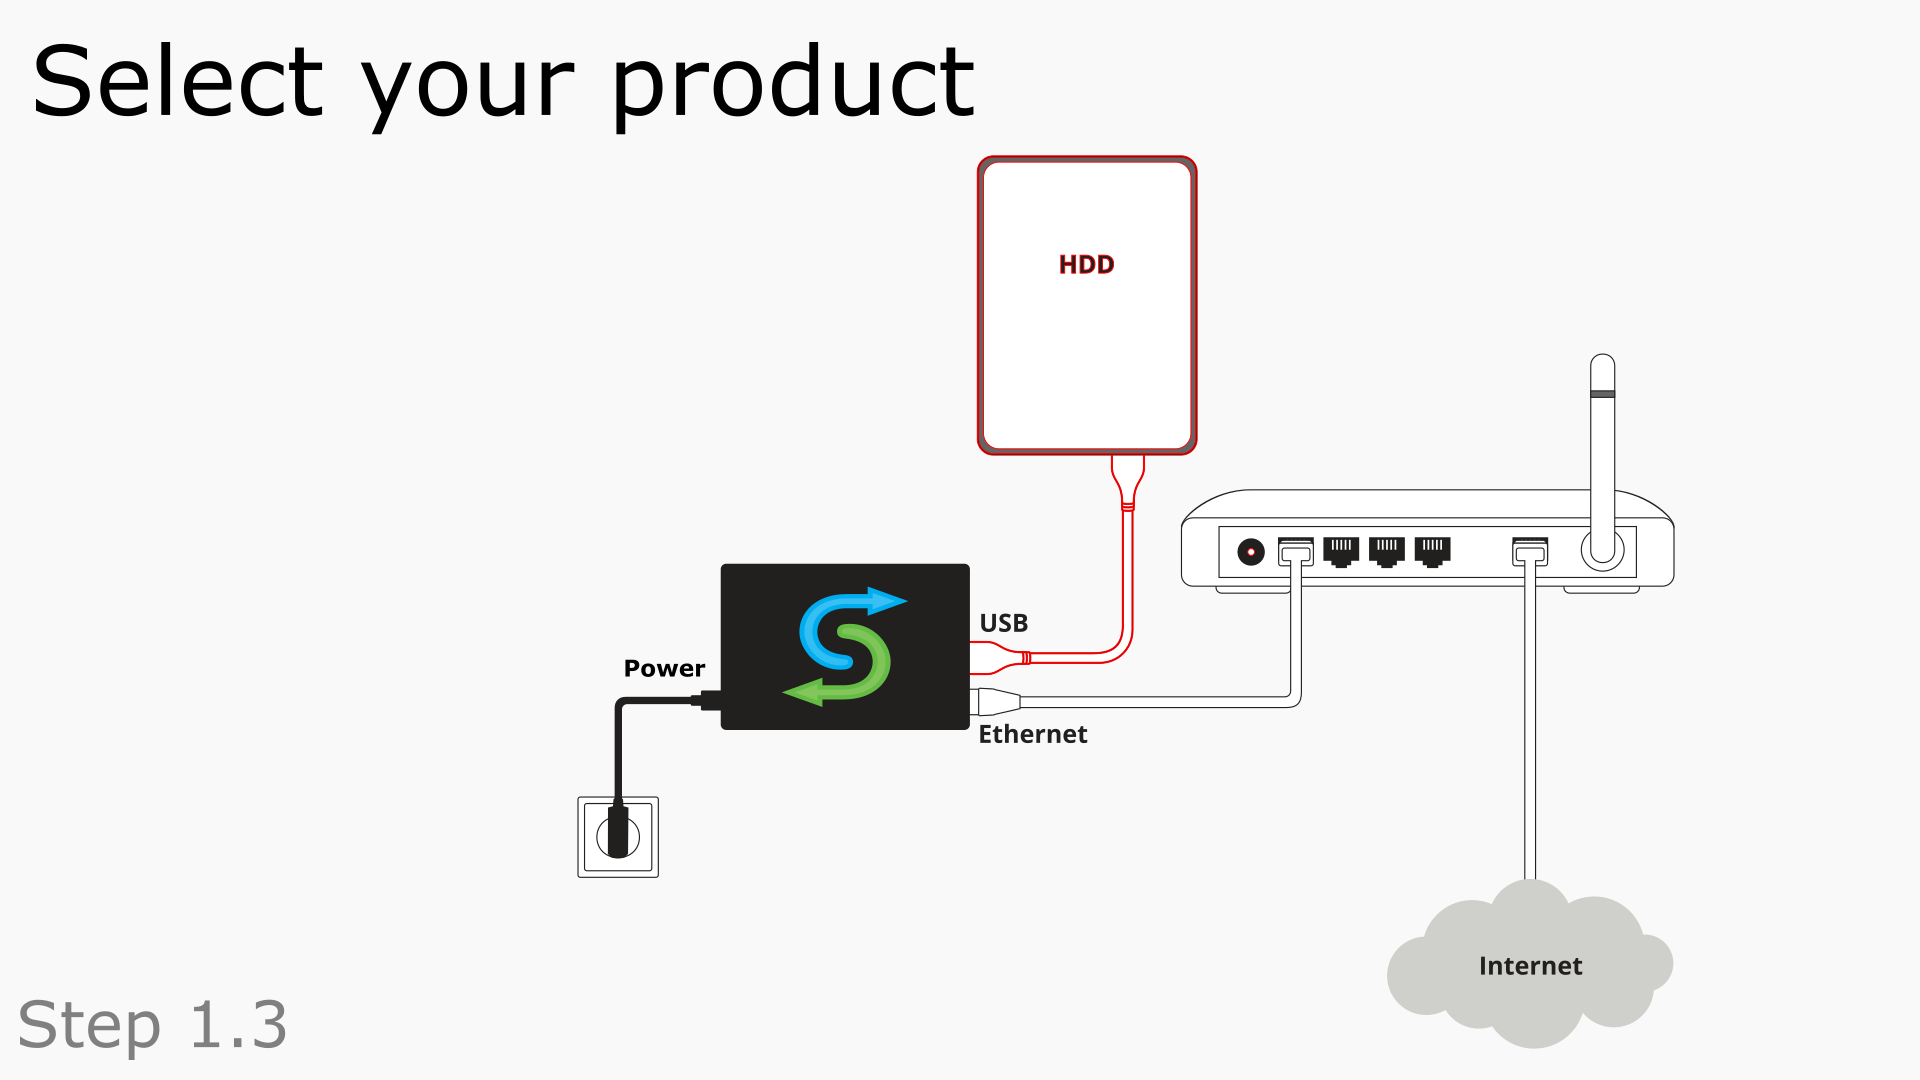
\includegraphics[width=0.7\linewidth]{../frames/15.png}
	\caption{One type, which requires an external storage.}
	\label{fig:6}
\end{figure}

\begin{figure}[htbp!]
	\centering
	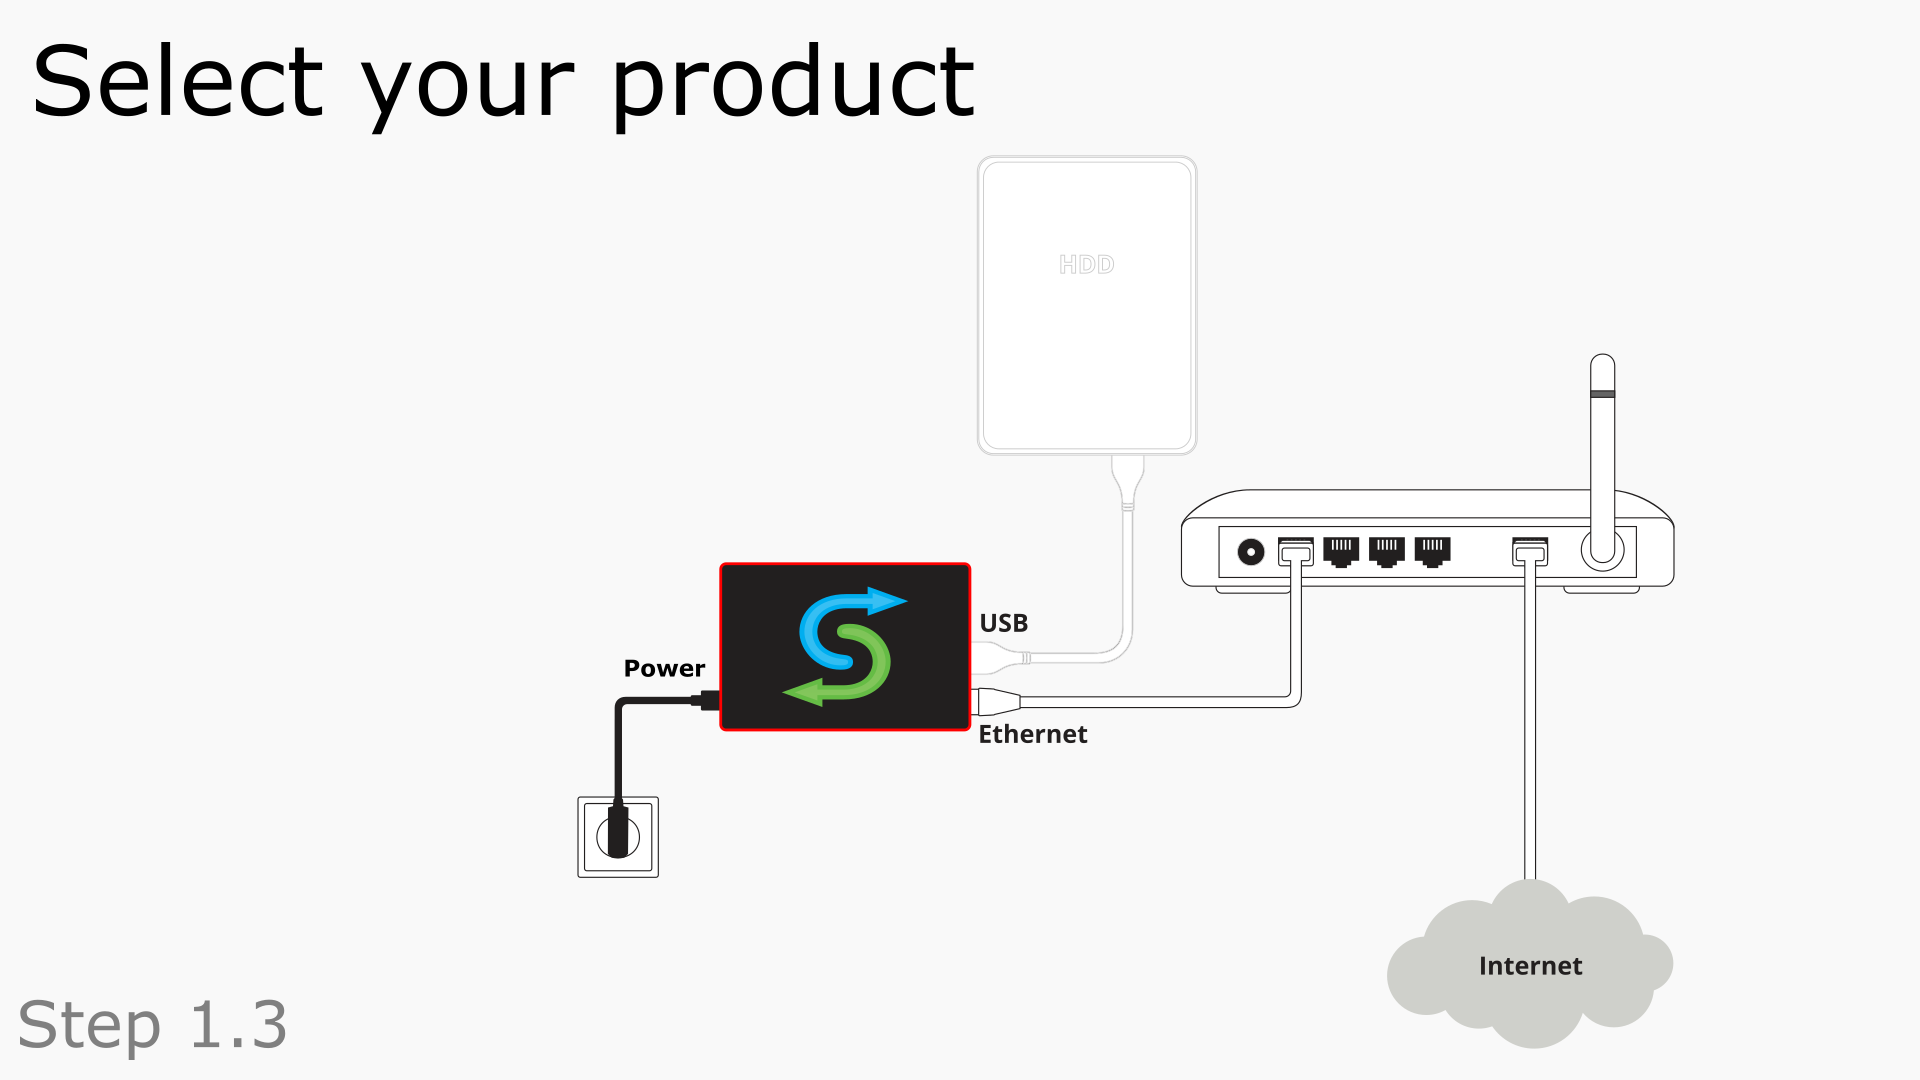
\includegraphics[width=0.7\linewidth]{../frames/16.png}
	\caption{And another type, which has already an internal storage and does not require an external storage. However, you can still use an external storage if you want. Keep in mind, that you can use only one storage a time.}
	\label{fig:7}
\end{figure}

\begin{figure}[htbp!]
	\centering
	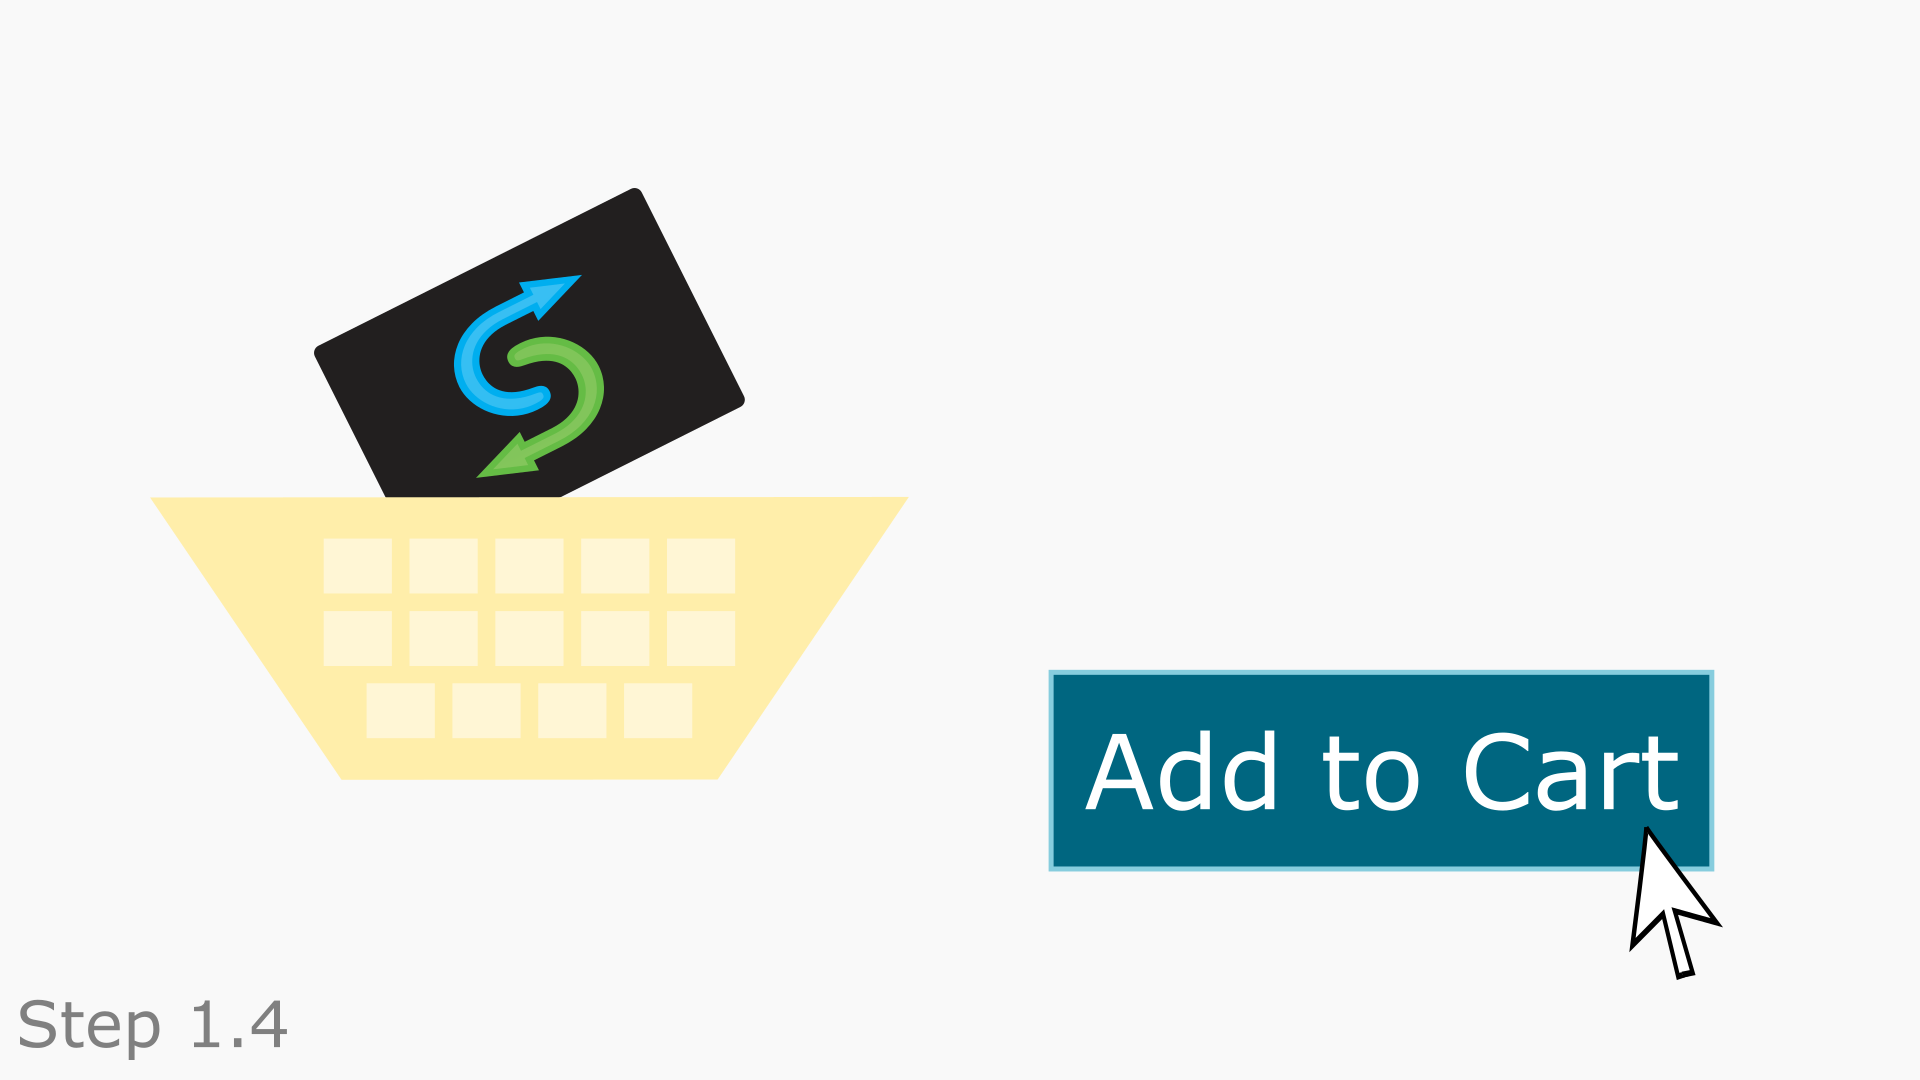
\includegraphics[width=0.7\linewidth]{../frames/18.png}
	\caption{Add the device of choice to the shopping cart.}
	\label{fig:8}
\end{figure}

\begin{figure}[htbp!]
	\centering
	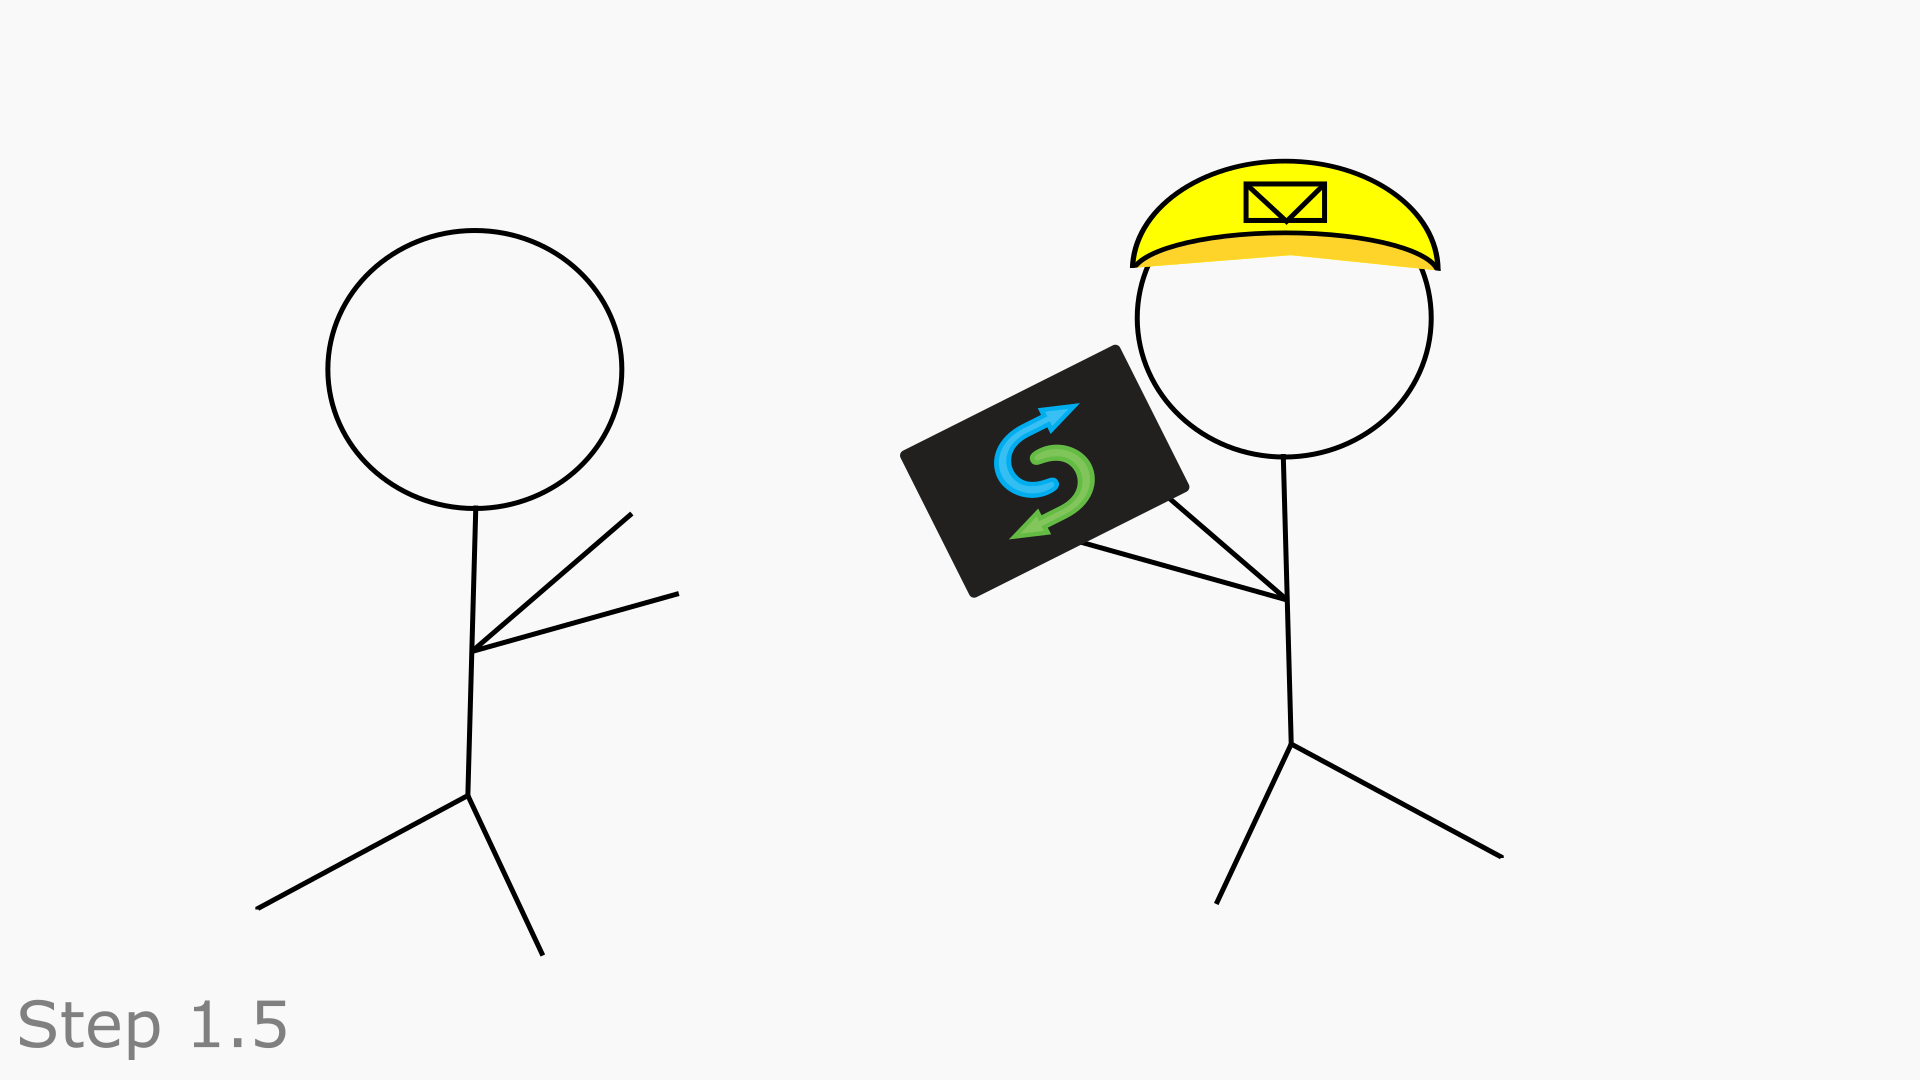
\includegraphics[width=0.7\linewidth]{../frames/19.png}
	\caption{Get your device delivered to any country.}
	\label{fig:9}
\end{figure}

\begin{figure}[htbp!]
	\centering
	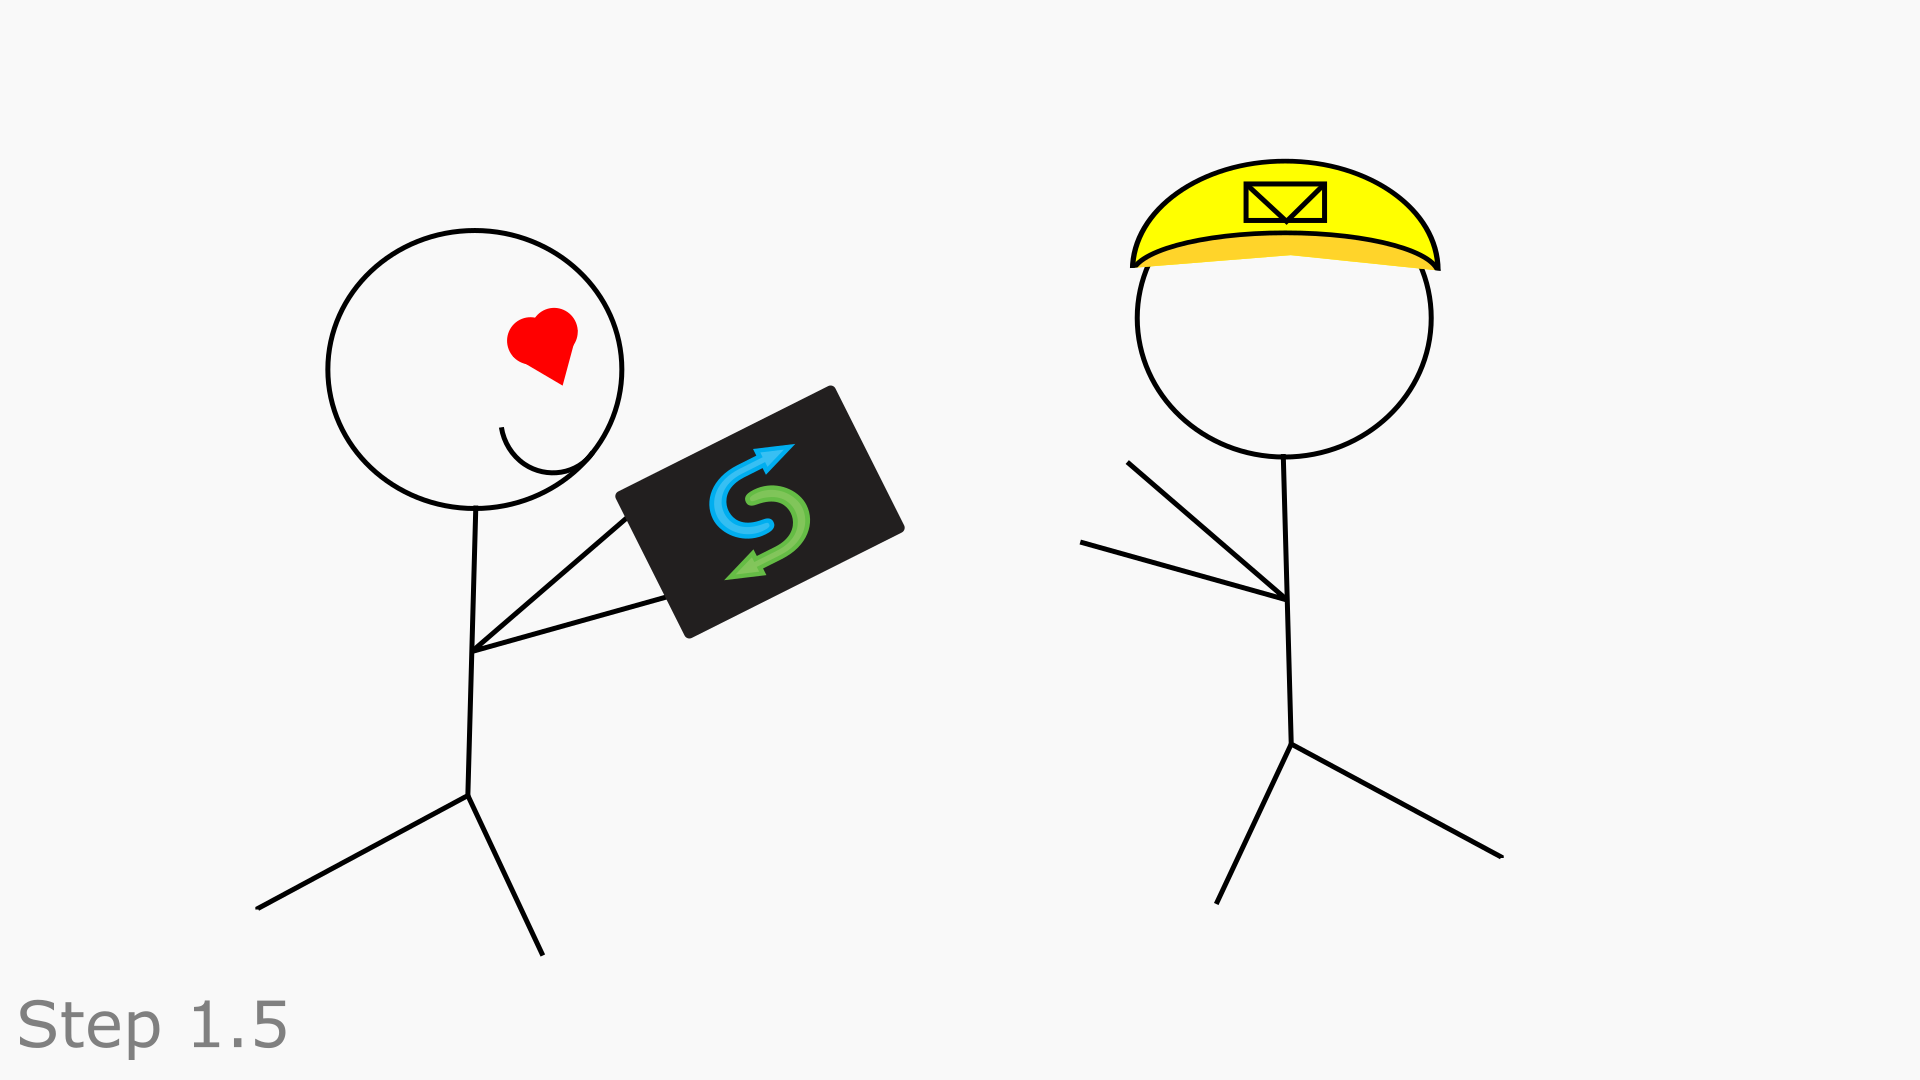
\includegraphics[width=0.7\linewidth]{../frames/21.png}
	\caption{And fall in love, when you hold it first time in your hands.}
	\label{fig:10}
\end{figure}

\section{Connect Everything}

\begin{figure}[htbp!]
	\centering
	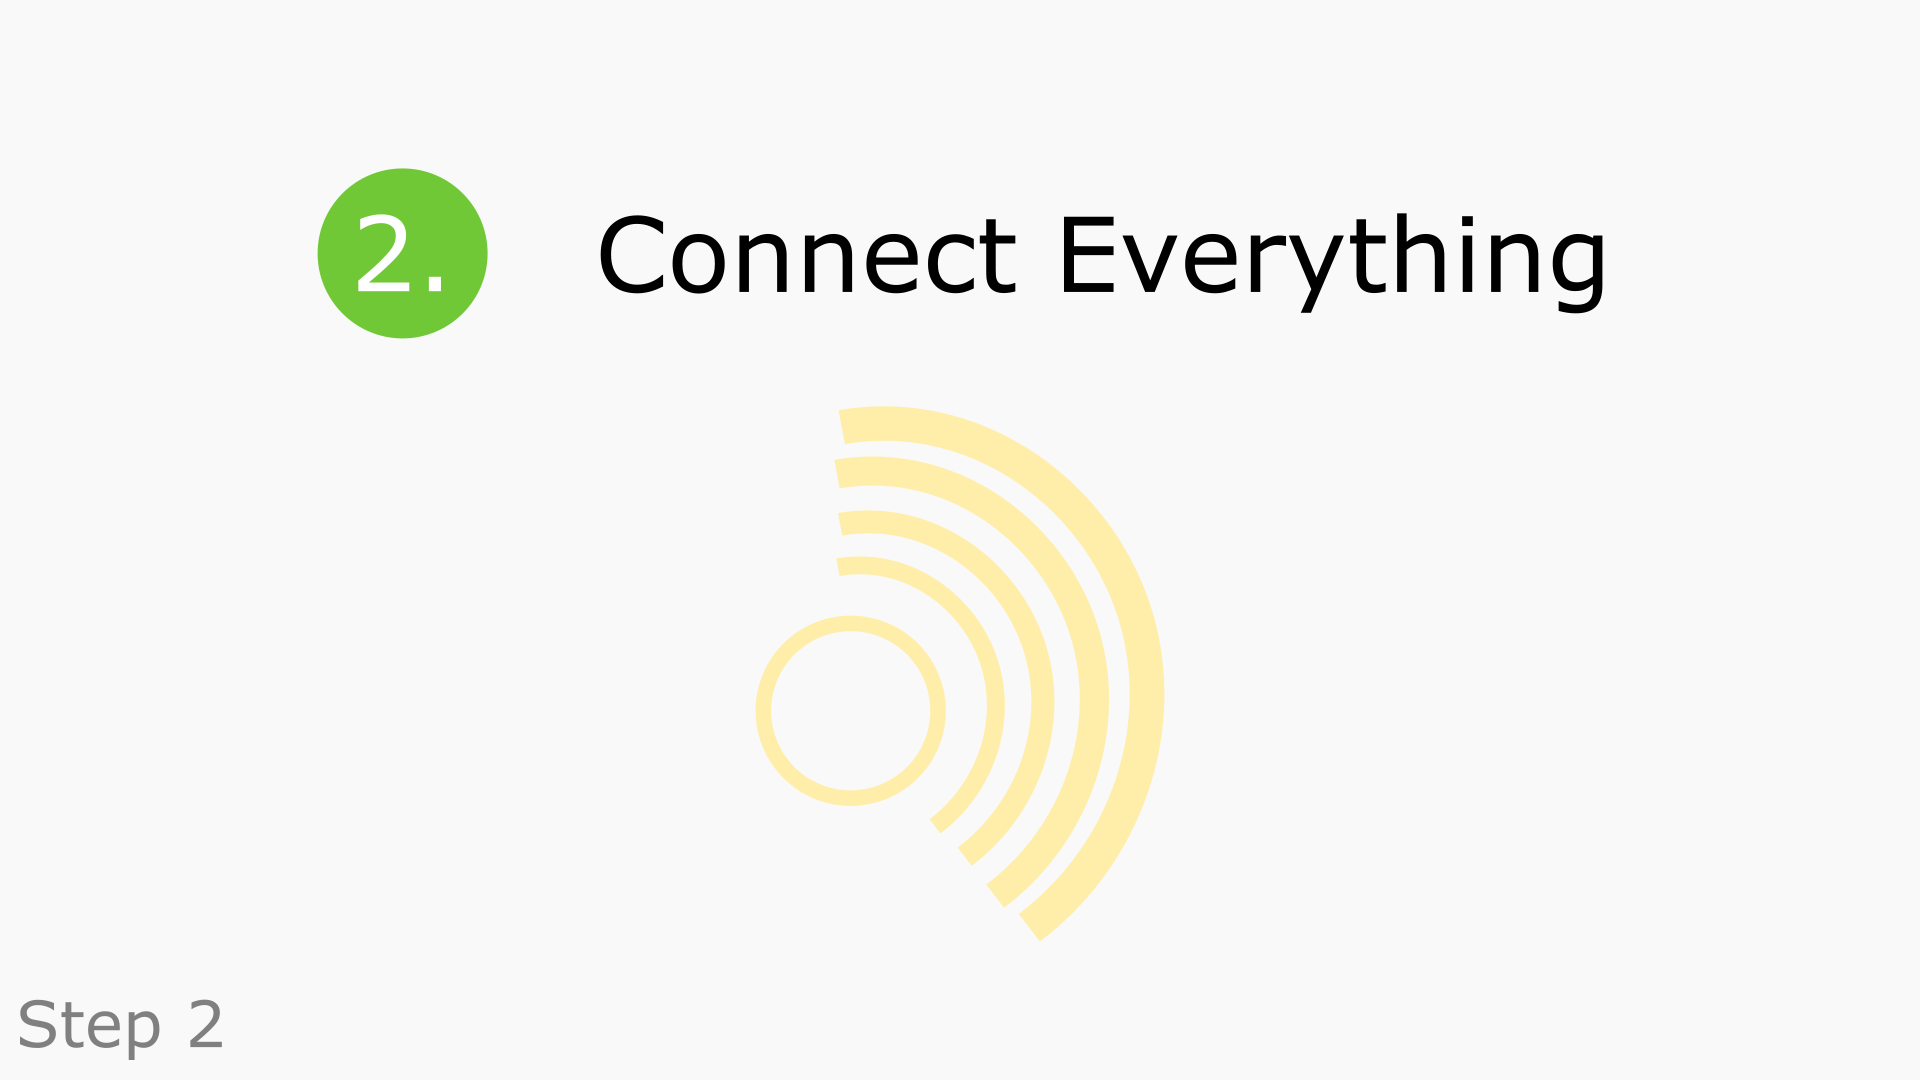
\includegraphics[width=0.7\linewidth]{../frames/22.png}
	\caption{In a second step, you must connect everything.}
	\label{fig:11}
\end{figure}

\begin{figure}[htbp!]
	\centering
	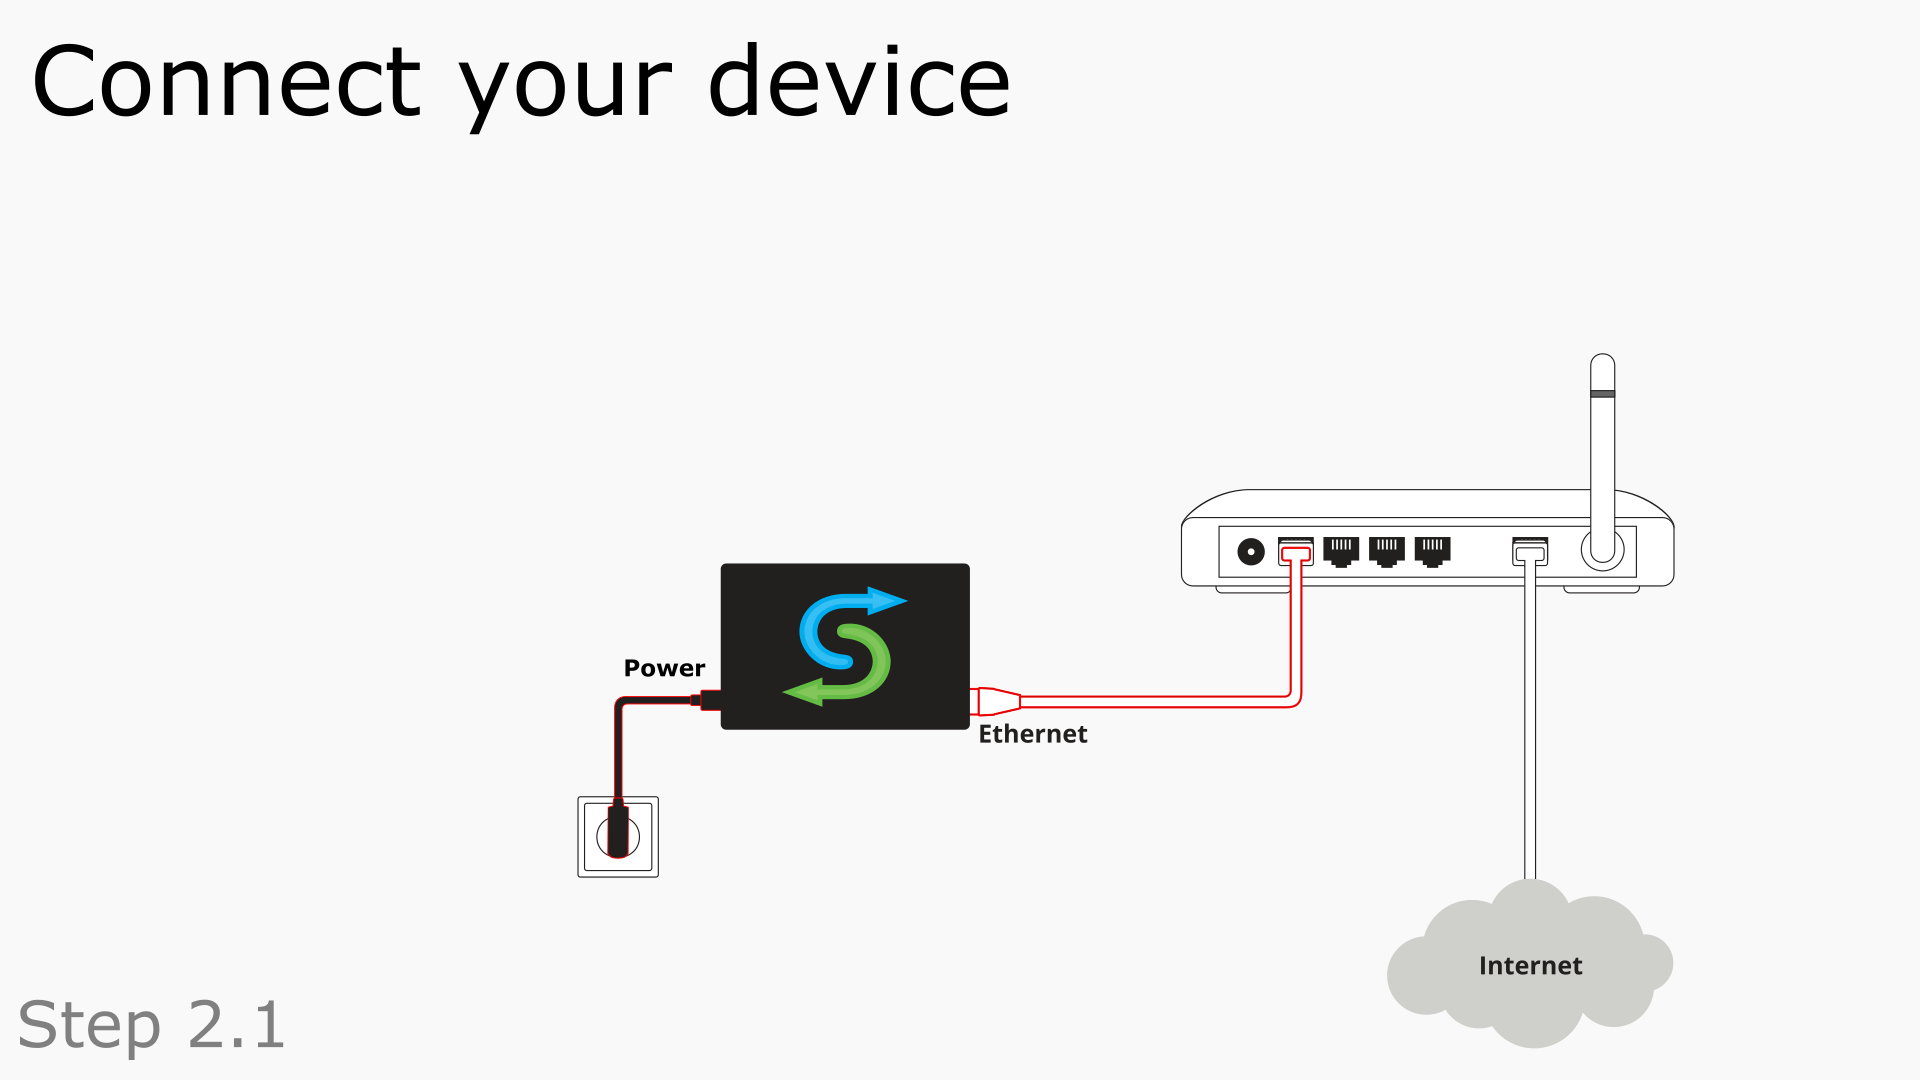
\includegraphics[width=0.7\linewidth]{../frames/23.png}
	\caption{Plug in your device to power supply and connect it with your router by a ethernet cable.}
	\label{fig:12}
\end{figure}

\begin{figure}[htbp!]
	\centering
	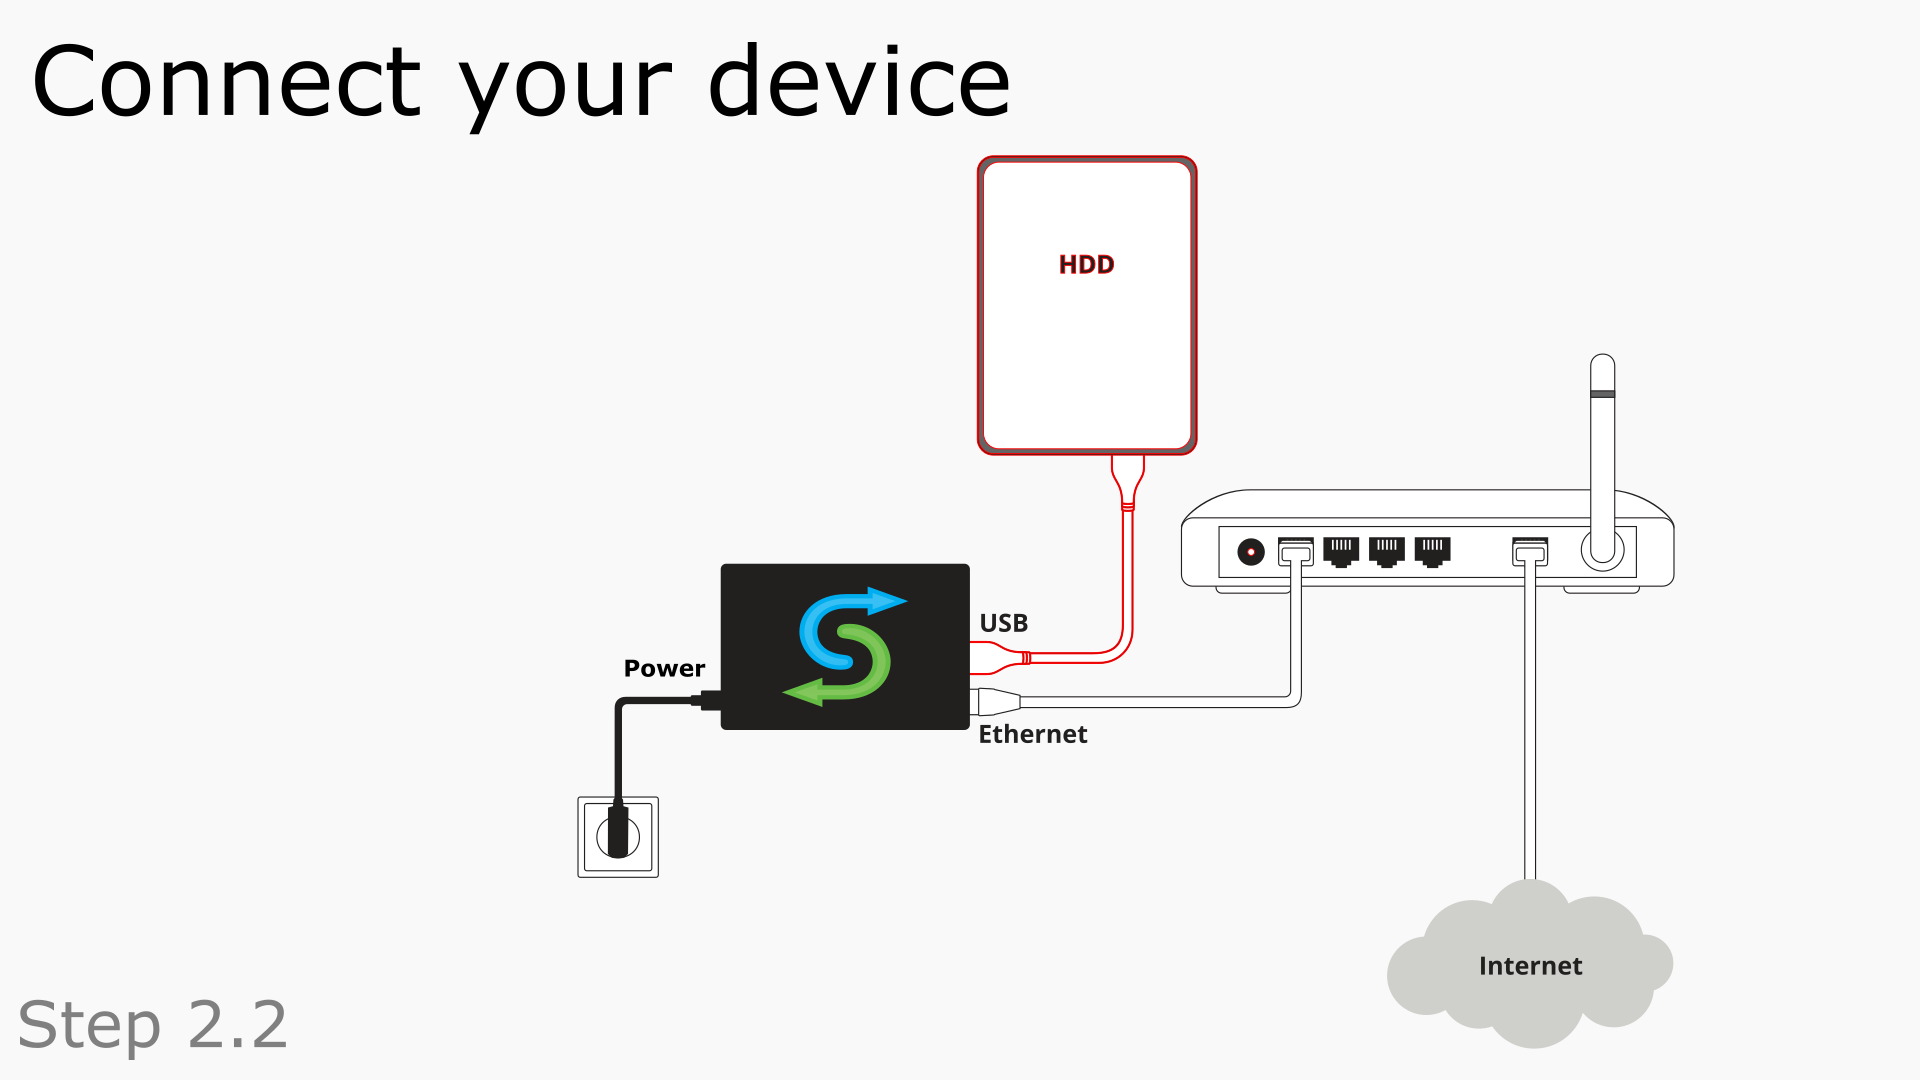
\includegraphics[width=0.7\linewidth]{../frames/24.png}
	\caption{Depending on your device type, plug in an external storage, as well.}
	\label{fig:13}
\end{figure}

\section{Activate}

\begin{figure}[htbp!]
	\centering
	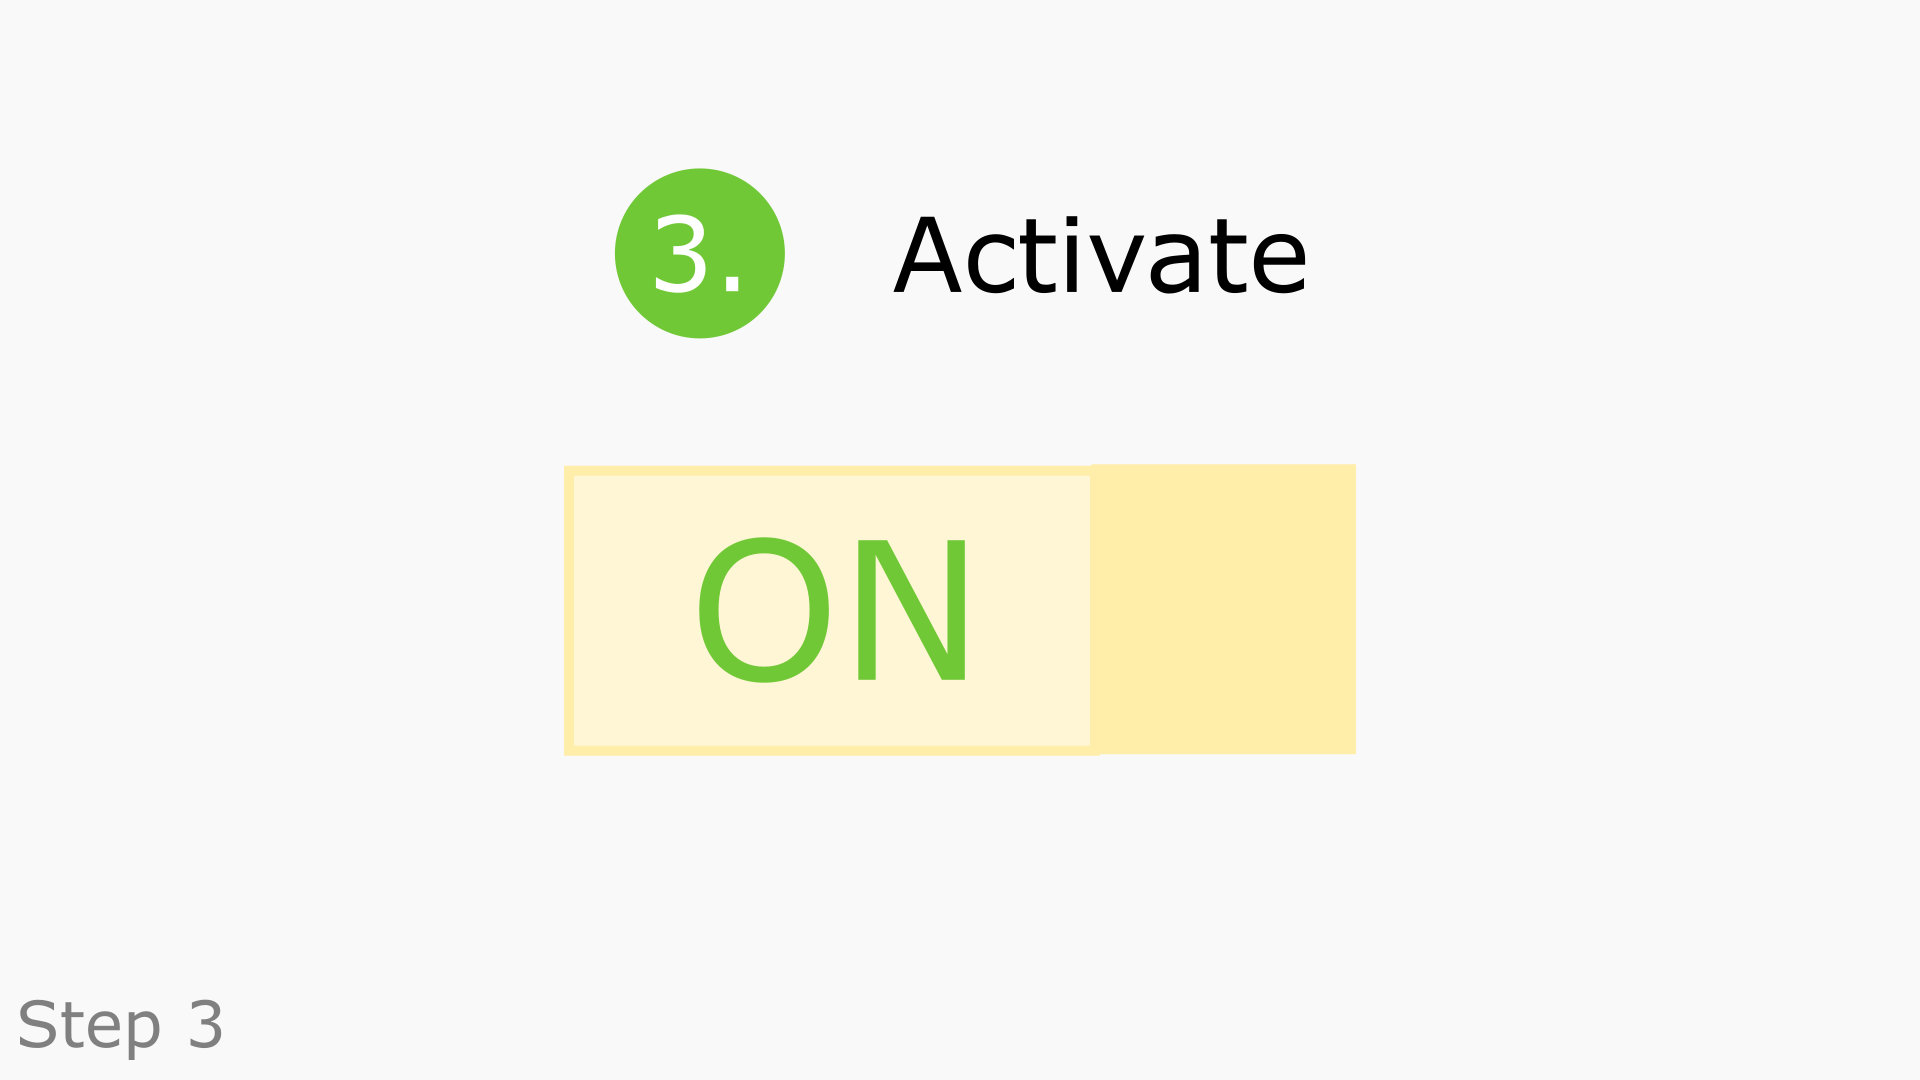
\includegraphics[width=0.7\linewidth]{../frames/26.png}
	\caption{Now, there comes the activation.}
	\label{fig:14}
\end{figure}

\begin{figure}[htbp!]
	\centering
	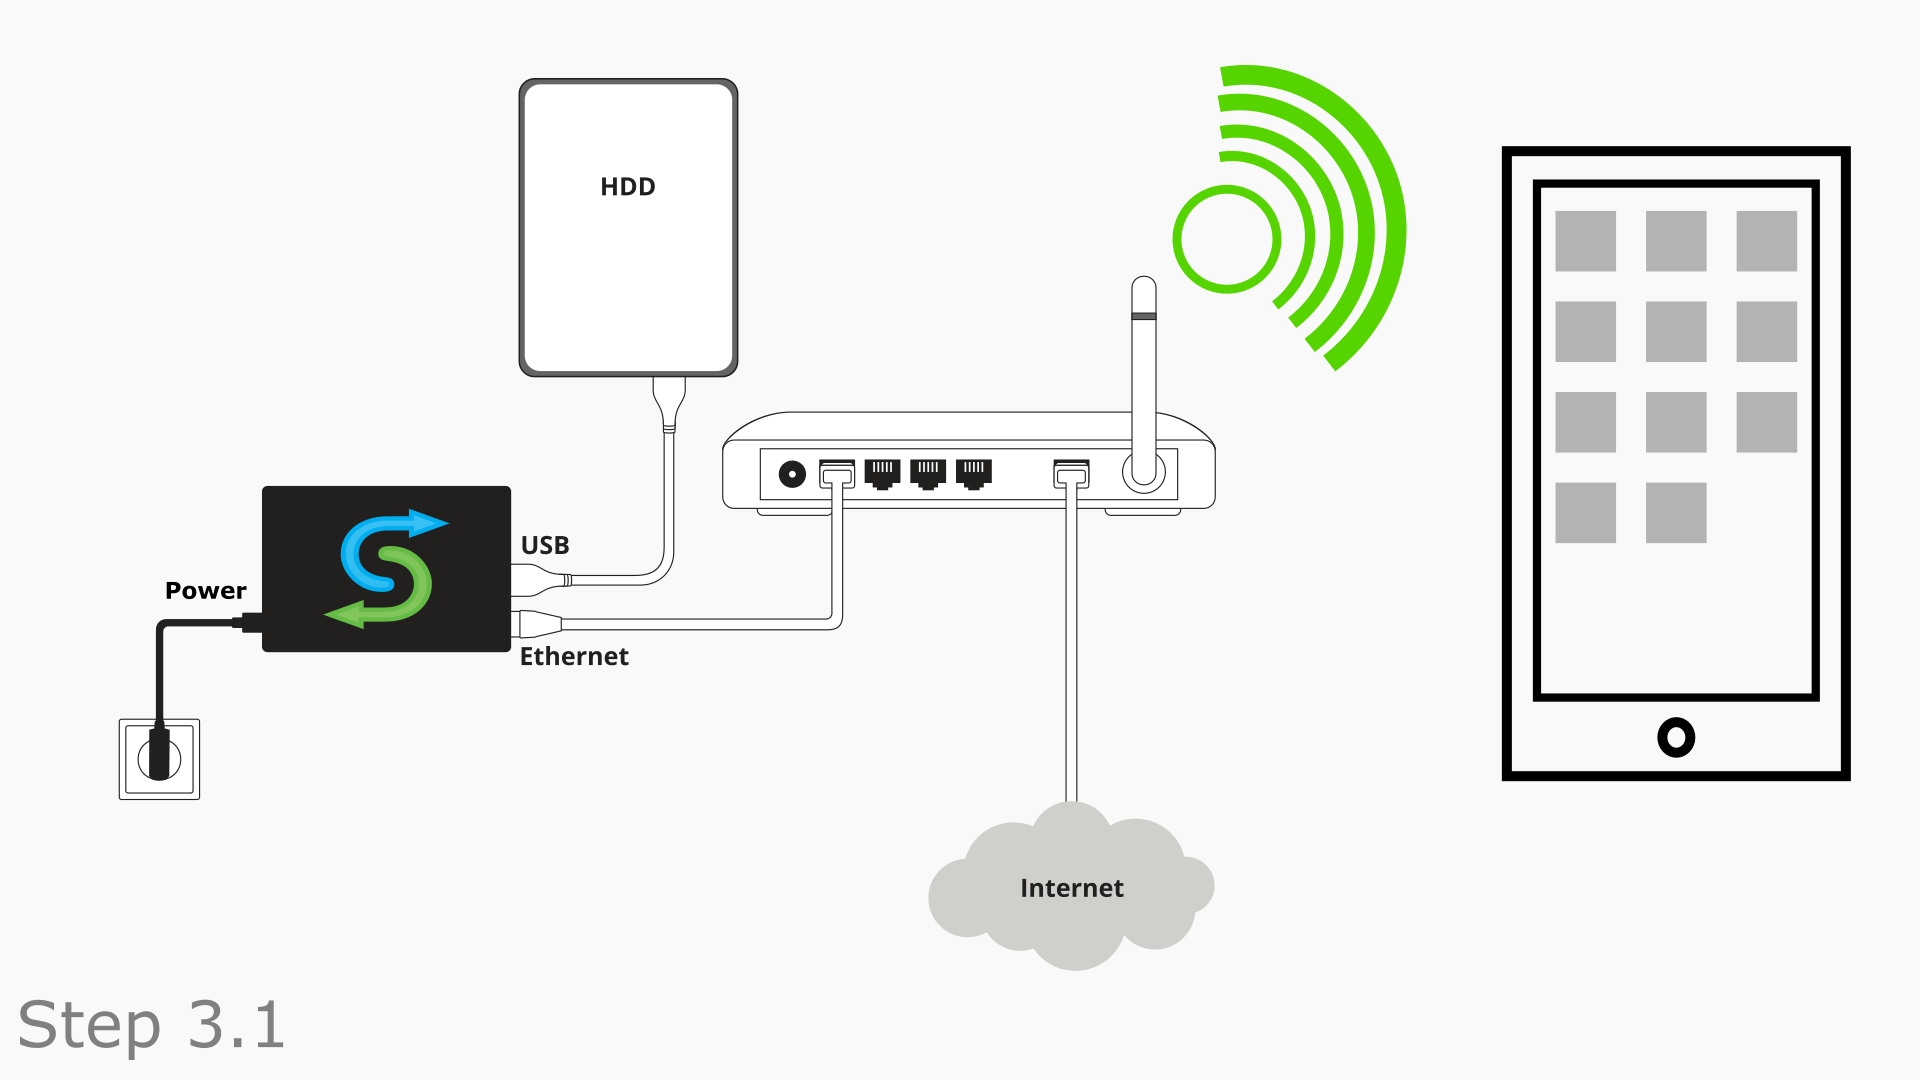
\includegraphics[width=0.7\linewidth]{../frames/27.png}
	\caption{Connect your smartphone to the Wifi of your router.}
	\label{fig:15}
\end{figure}

\begin{figure}[htbp!]
	\centering
	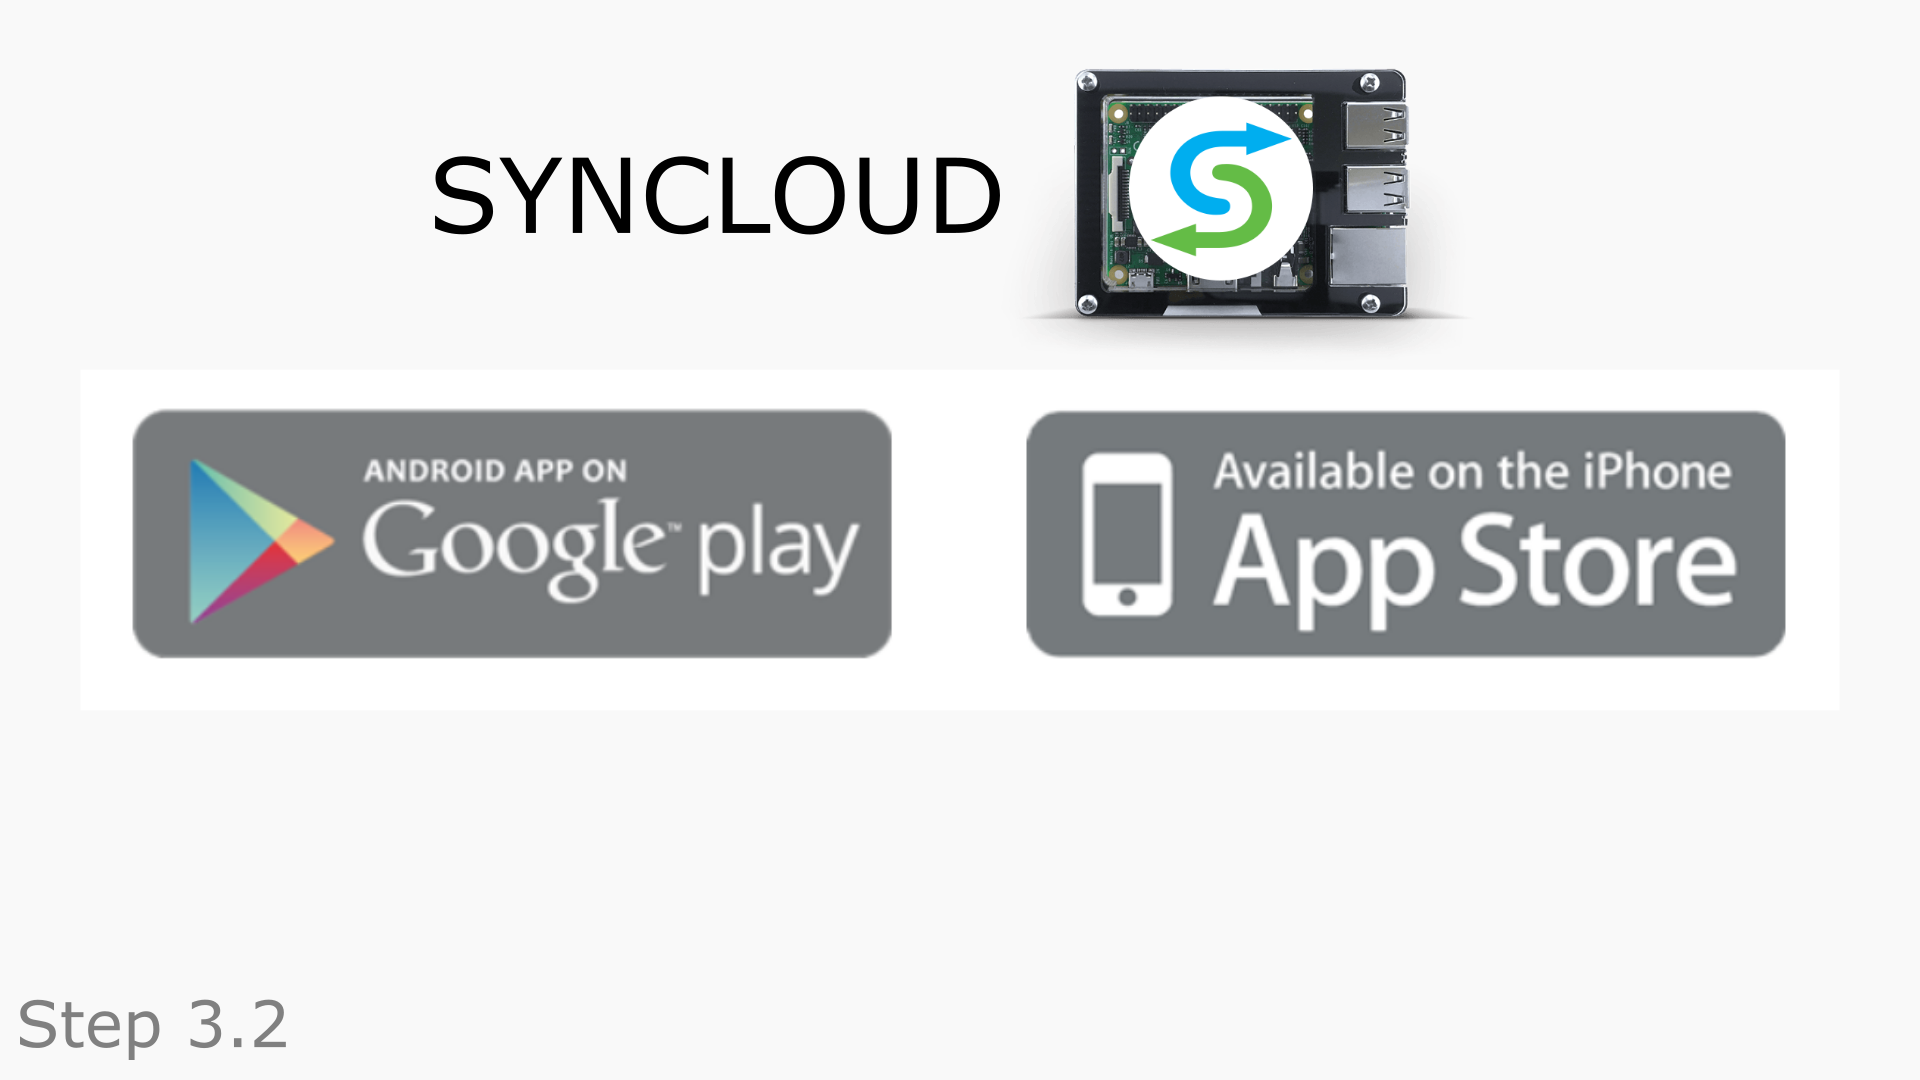
\includegraphics[width=0.7\linewidth]{../frames/28.png}
	\caption{Download our Syncloud app for Android or your I phone.}
	\label{fig:16}
\end{figure}

\begin{figure}[htbp!]
	\centering
	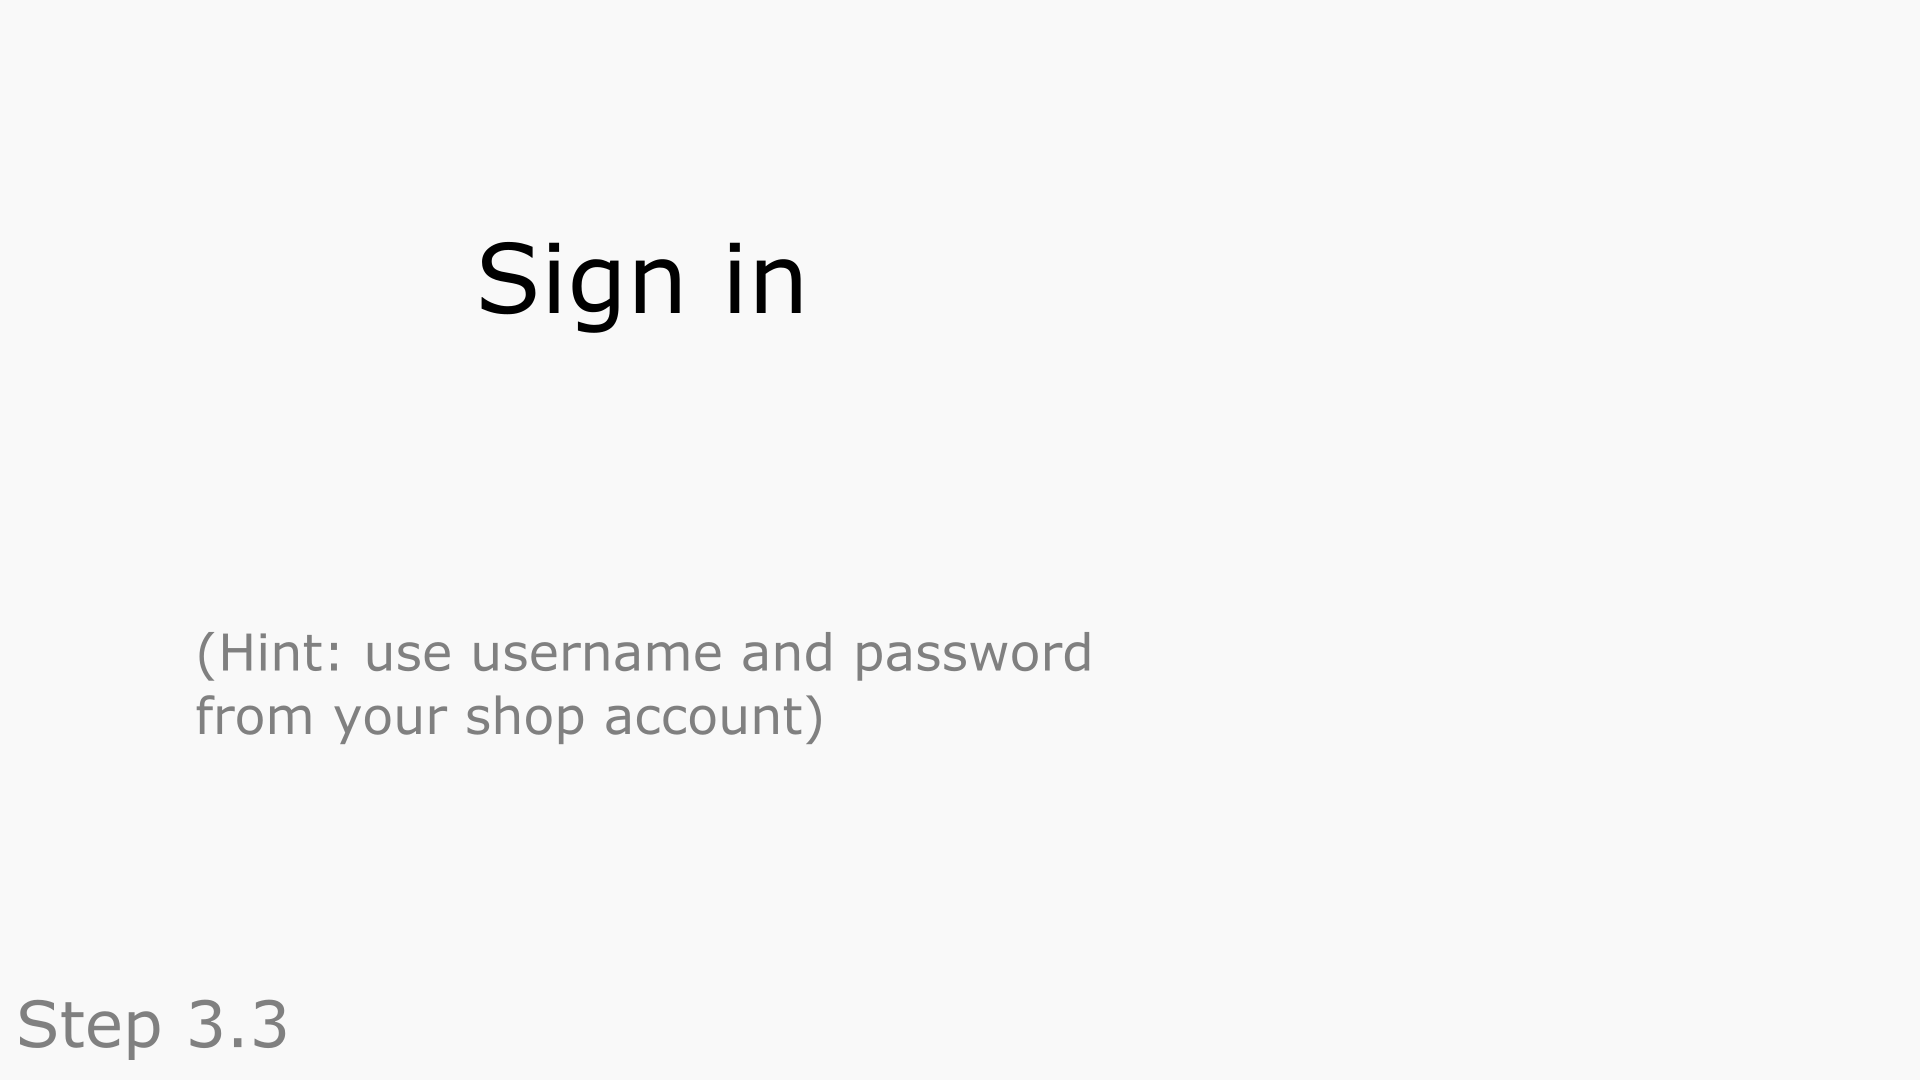
\includegraphics[width=0.7\linewidth]{../frames/29.png}
	\caption{Open the app and sign in. You can use your username and password from your shop account.}
	\label{fig:17}
\end{figure}

\begin{figure}[htbp!]
	\centering
	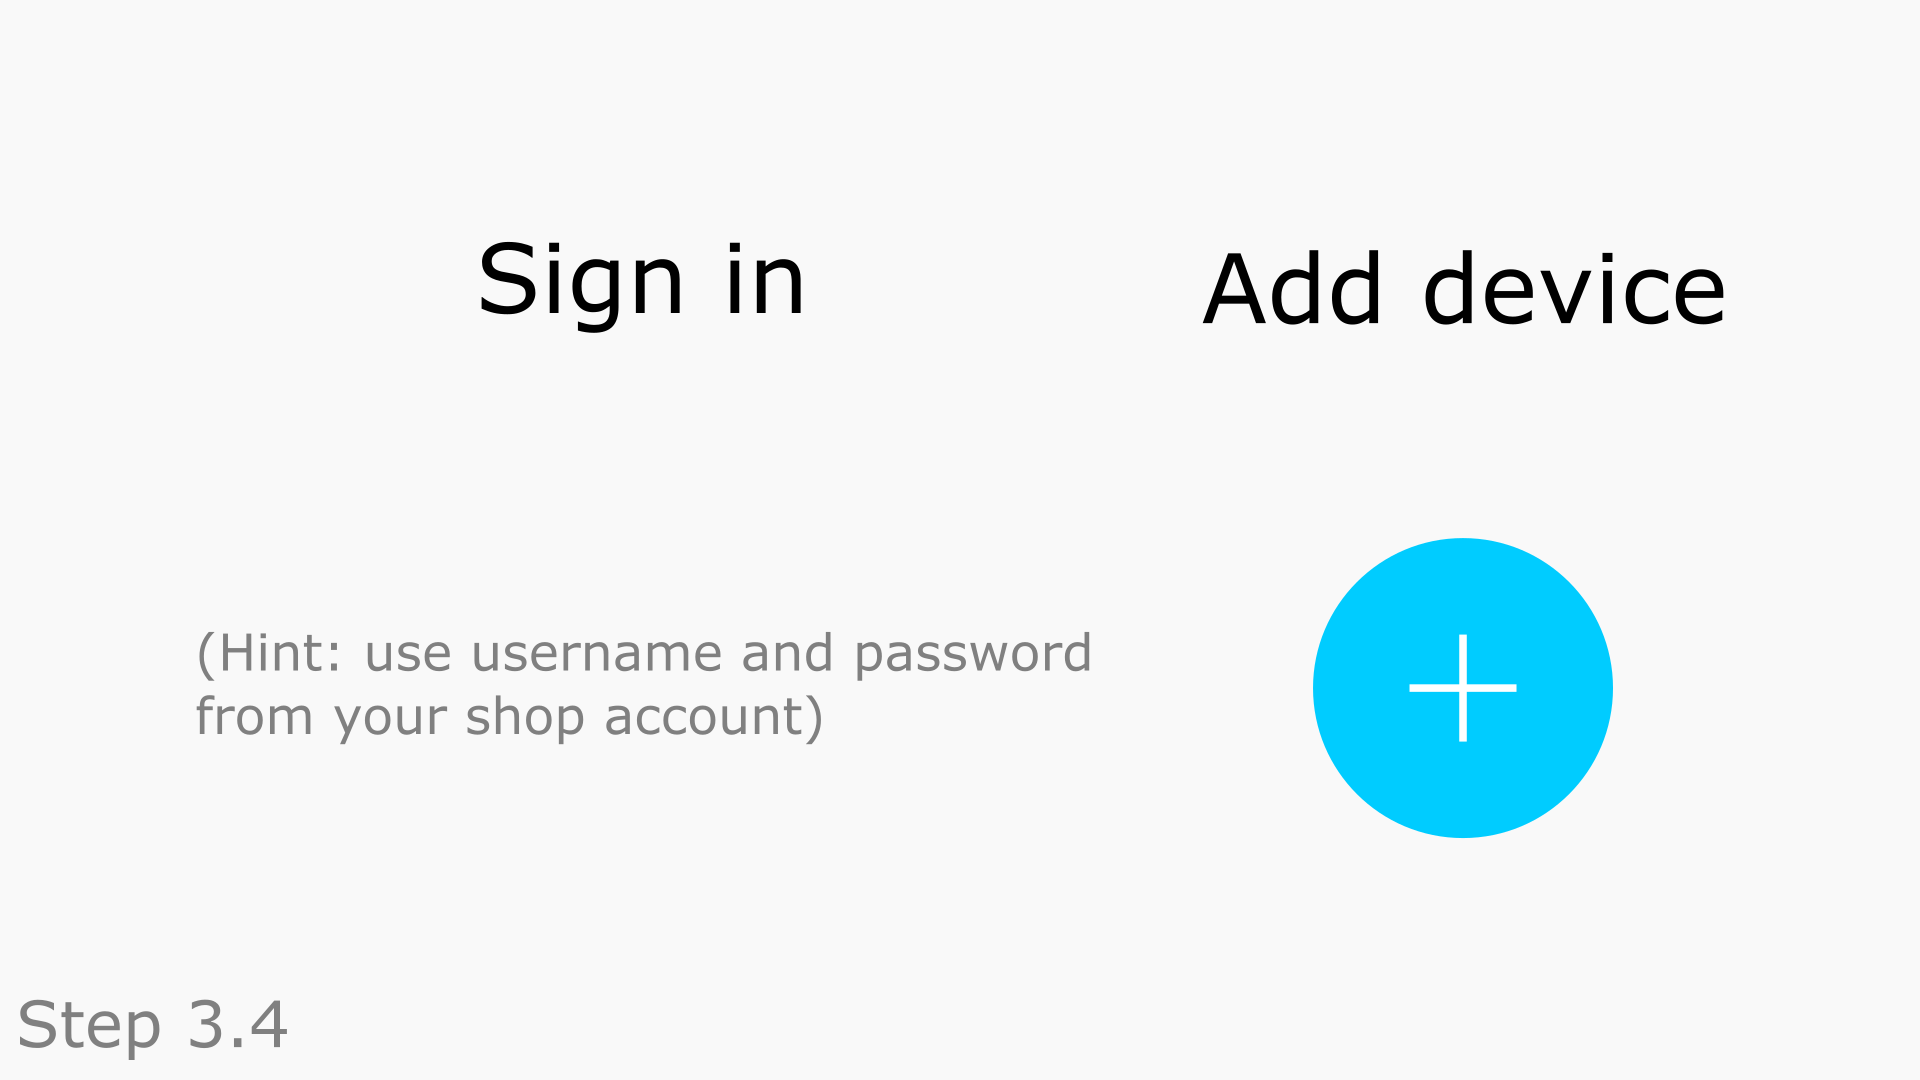
\includegraphics[width=0.7\linewidth]{../frames/30.png}
	\caption{Then, press the plus button to search your device. If you have found it, click on the device name.}
	\label{fig:18}
\end{figure}

\begin{figure}[htbp!]
	\centering
	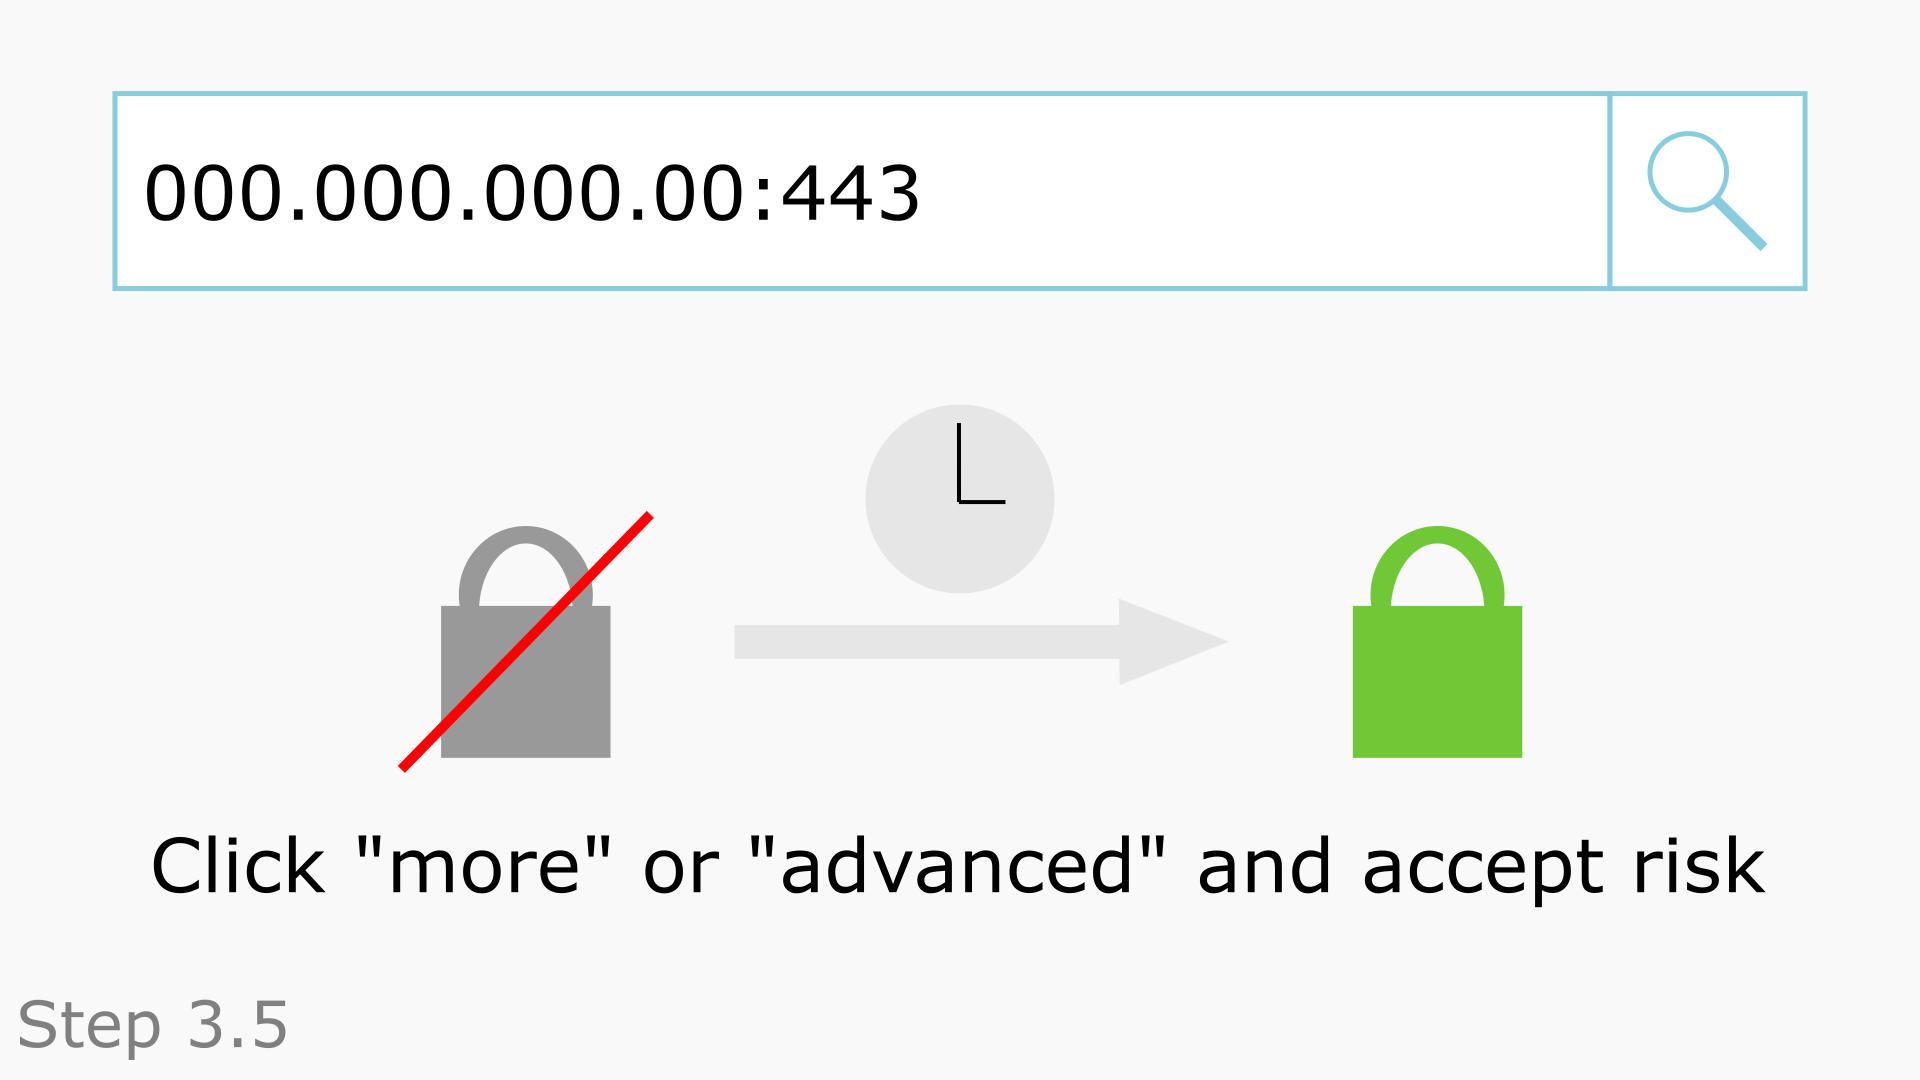
\includegraphics[width=0.7\linewidth]{../frames/31.png}
	\caption{Your browser will open, and the activation interface should appear. If there is a security warning, you can click on more or advanced and accept the risk.}
	\label{fig:19}
\end{figure}

\begin{figure}[htbp!]
	\centering
	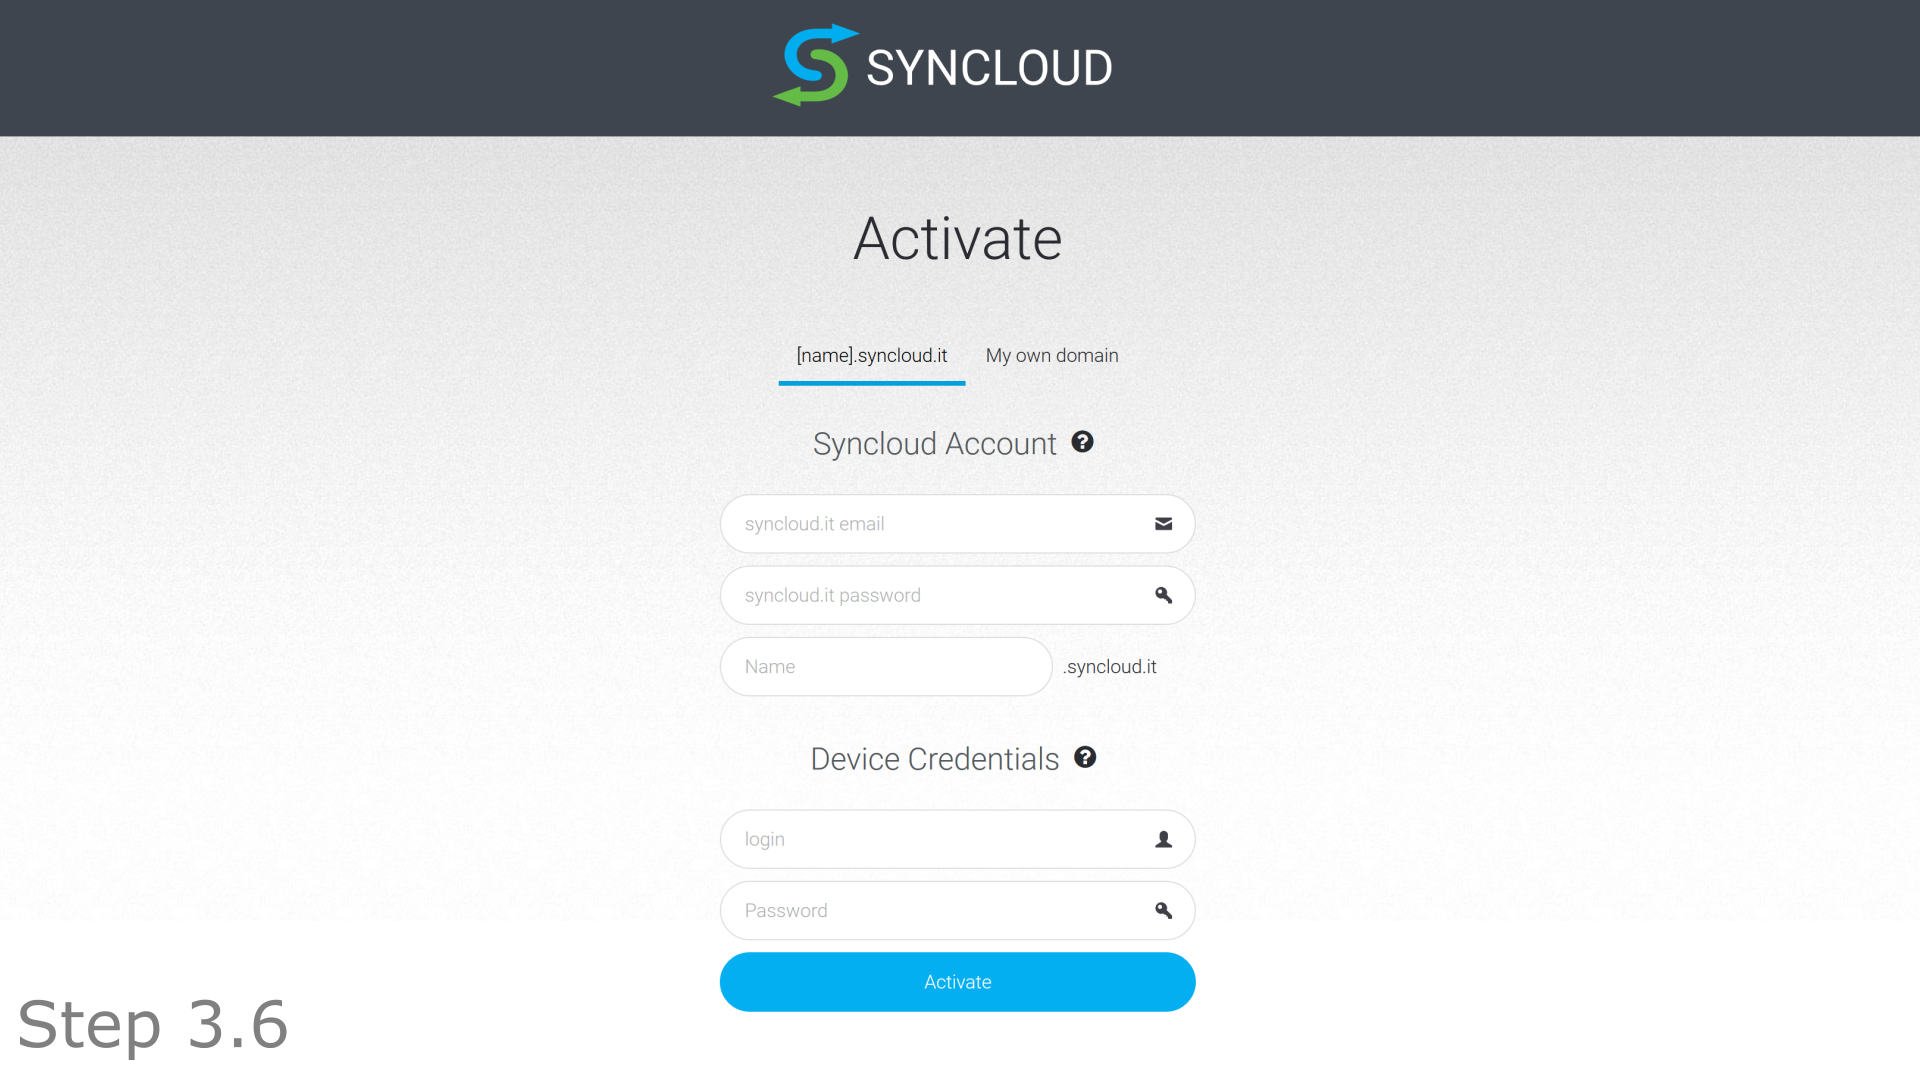
\includegraphics[width=0.7\linewidth]{../frames/32.png}
	\caption{You will see the activation interface.}
	\label{fig:20}
\end{figure}

\begin{figure}[htbp!]
	\centering
	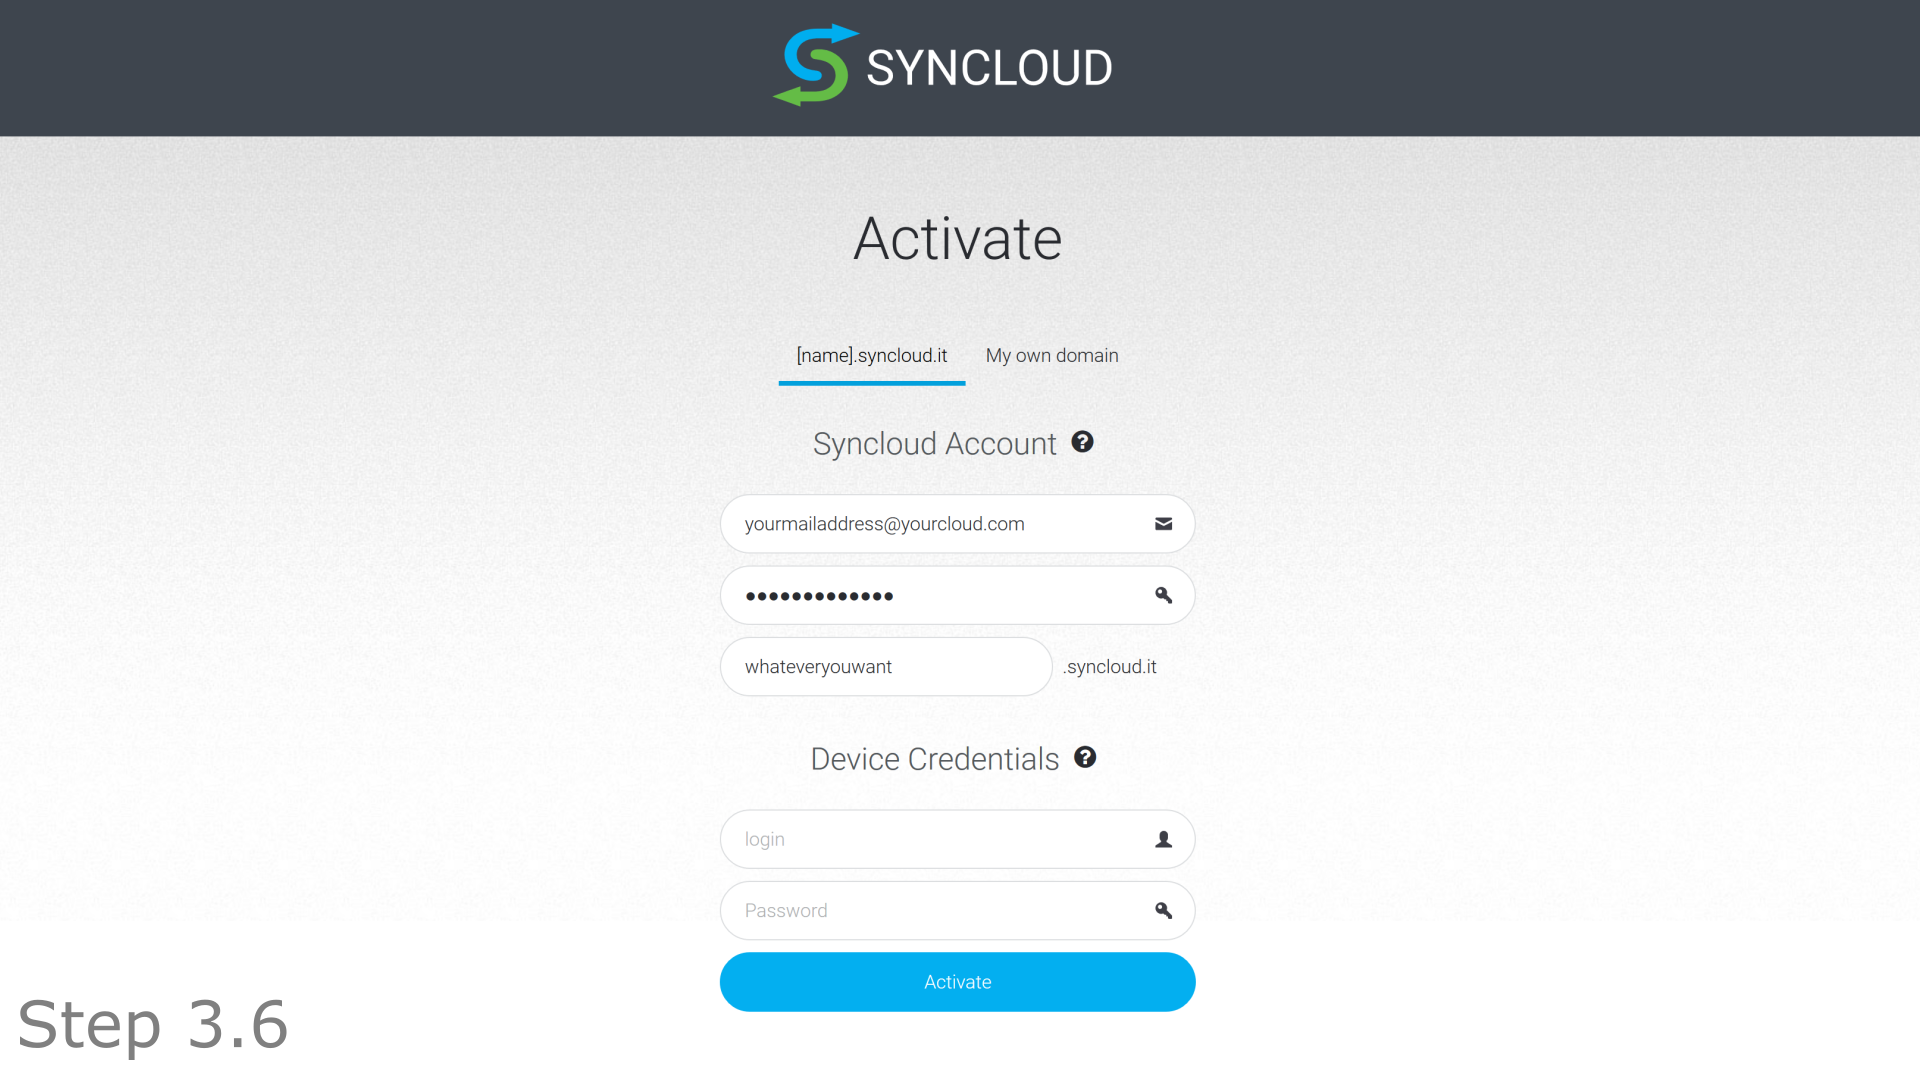
\includegraphics[width=0.7\linewidth]{../frames/33.png}
	\caption{Type in your e mail address and password same as in the shop or in the app. Type in a name you want to have for your device. With this URL, you will later access your device by the browser.}
	\label{fig:21}
\end{figure}

\begin{figure}[htbp!]
	\centering
	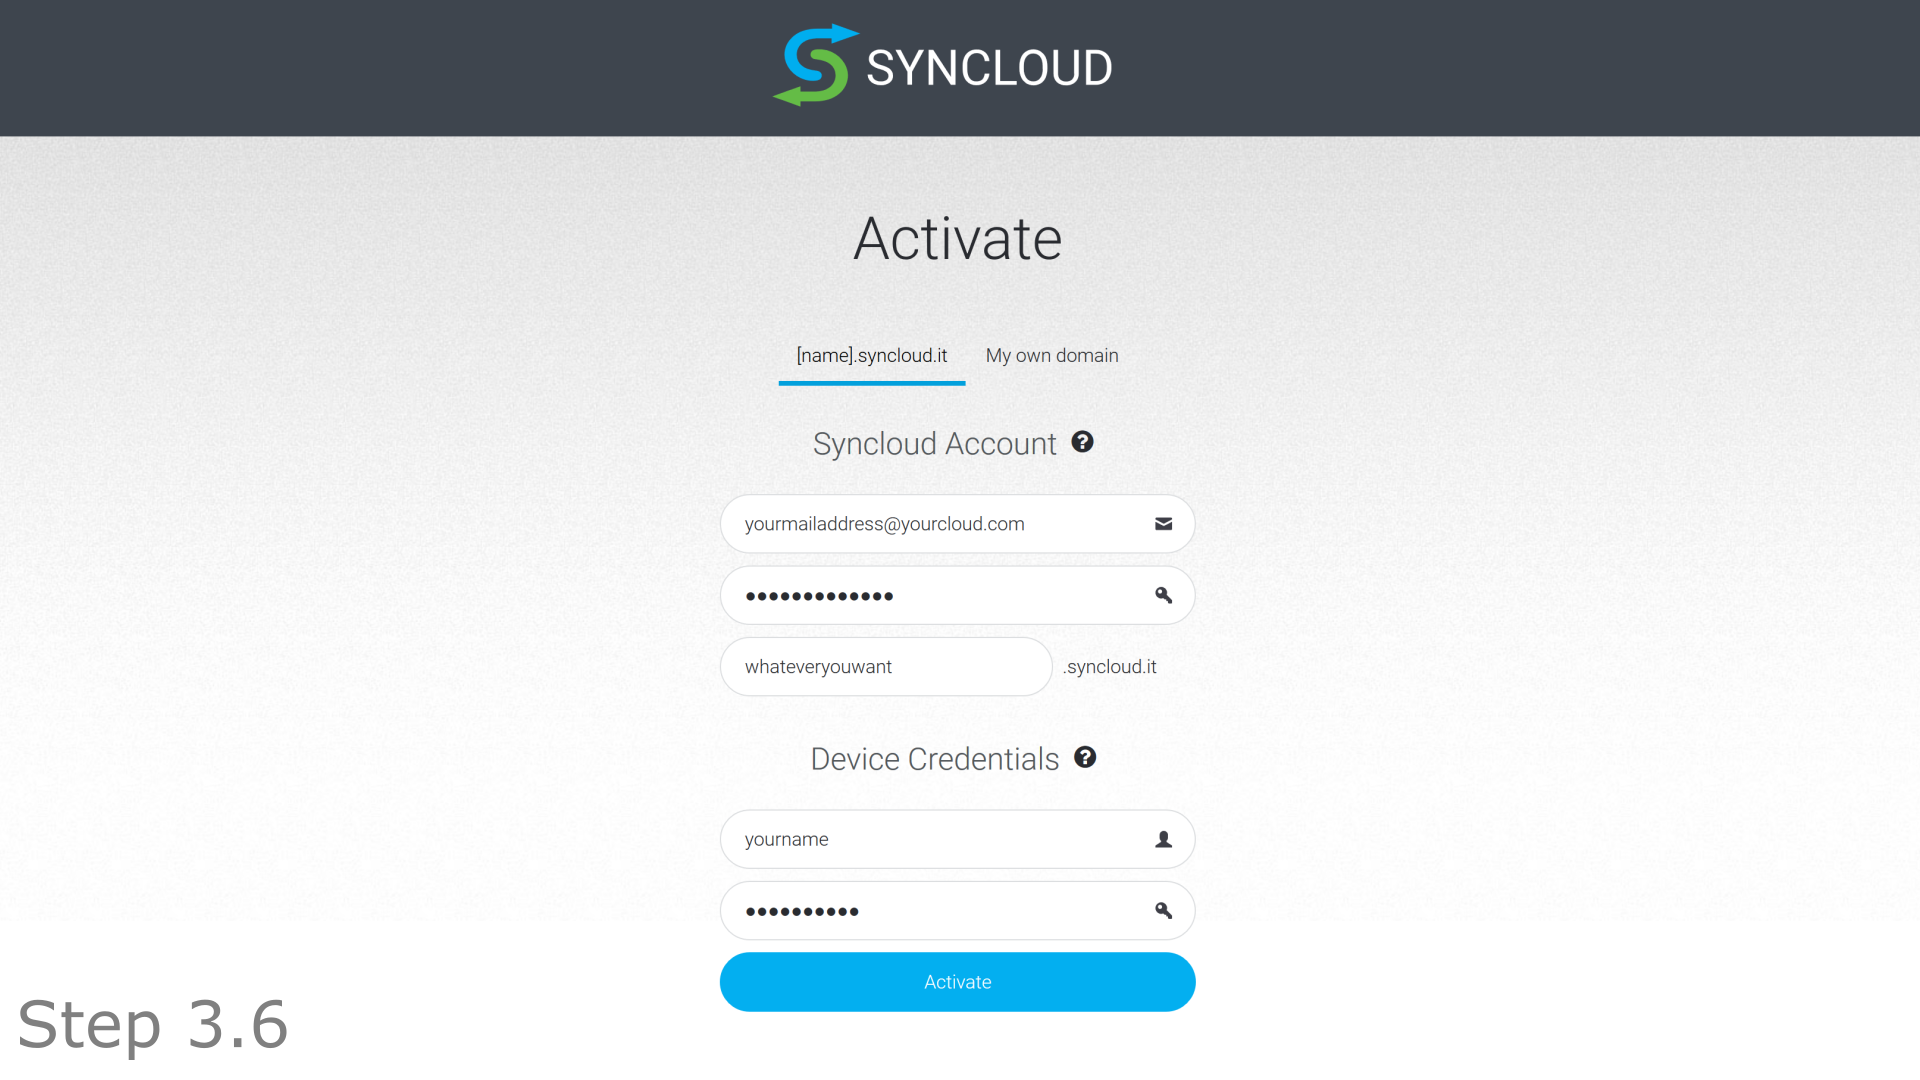
\includegraphics[width=0.7\linewidth]{../frames/34.png}
	\caption{Create then an account with which you can sign into your device later. Use any username and password.}
	\label{fig:22}
\end{figure}

\begin{figure}[htbp!]
	\centering
	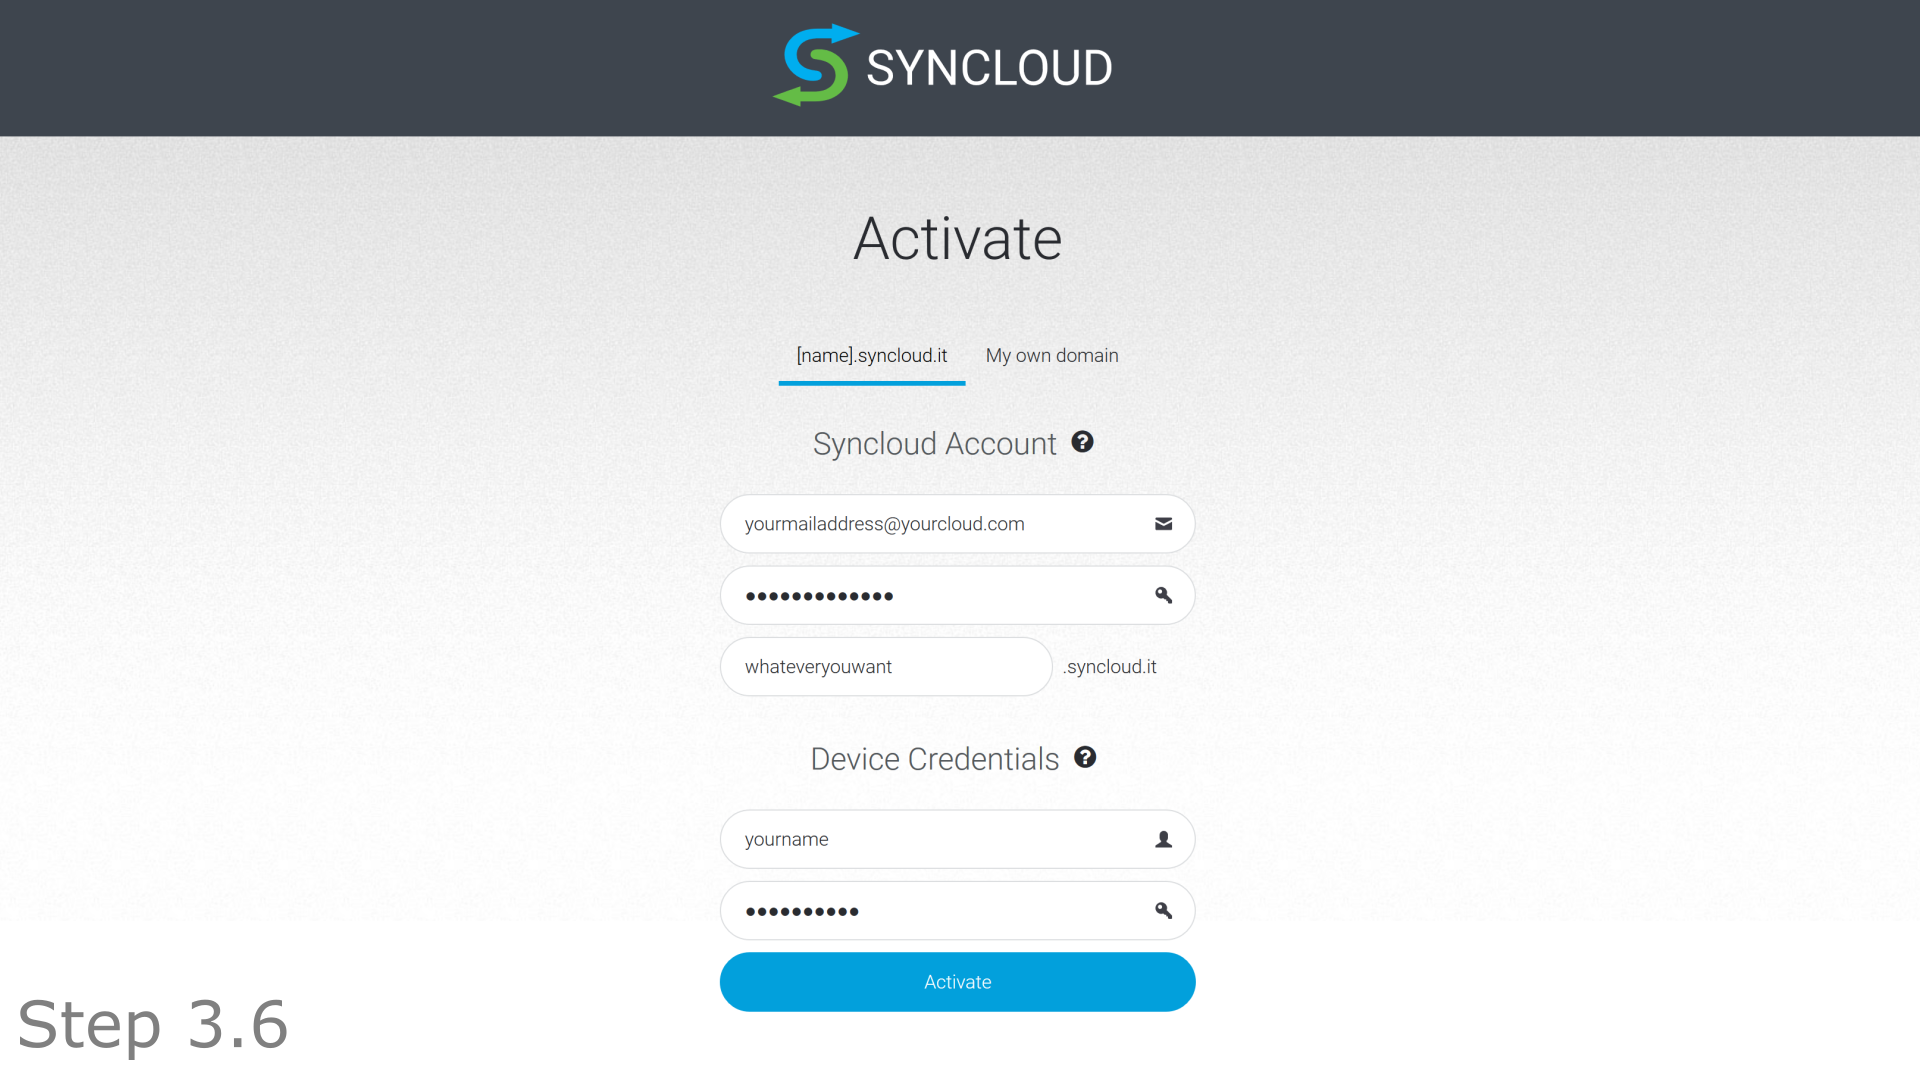
\includegraphics[width=0.7\linewidth]{../frames/35.png}
	\caption{Press then activation. This can take a few minutes.}
	\label{fig:23}
\end{figure}

\begin{figure}[htbp!]
	\centering
	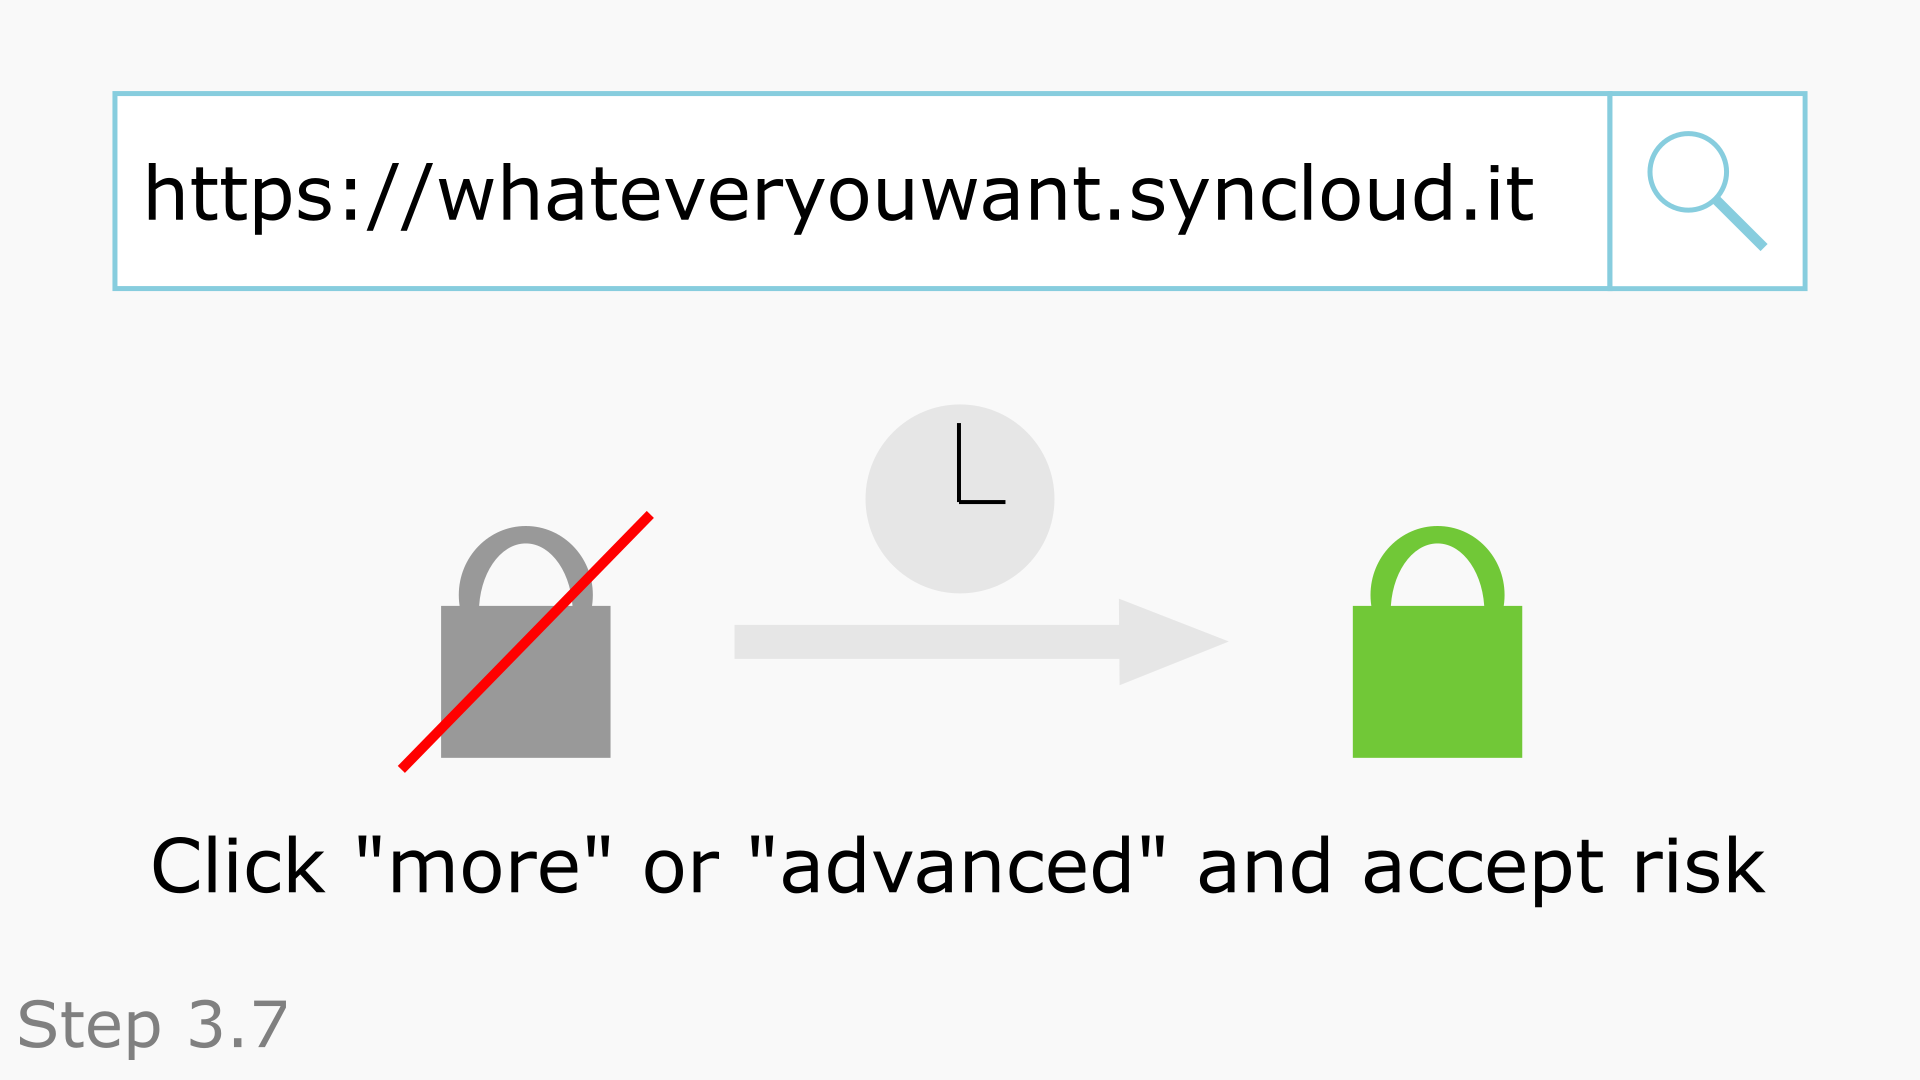
\includegraphics[width=0.7\linewidth]{../frames/36.png}
	\caption{After that, you will get redirect to your device user interface with your chosen URL. Same issue again, if there is a security warning, you can click on more or advanced and accept the risk. A certificate will be created for you soon to allow a secure access to your device. If you don’t have a certificate till next day, please contact our support.}
	\label{fig:24}
\end{figure}

\begin{figure}[htbp!]
	\centering
	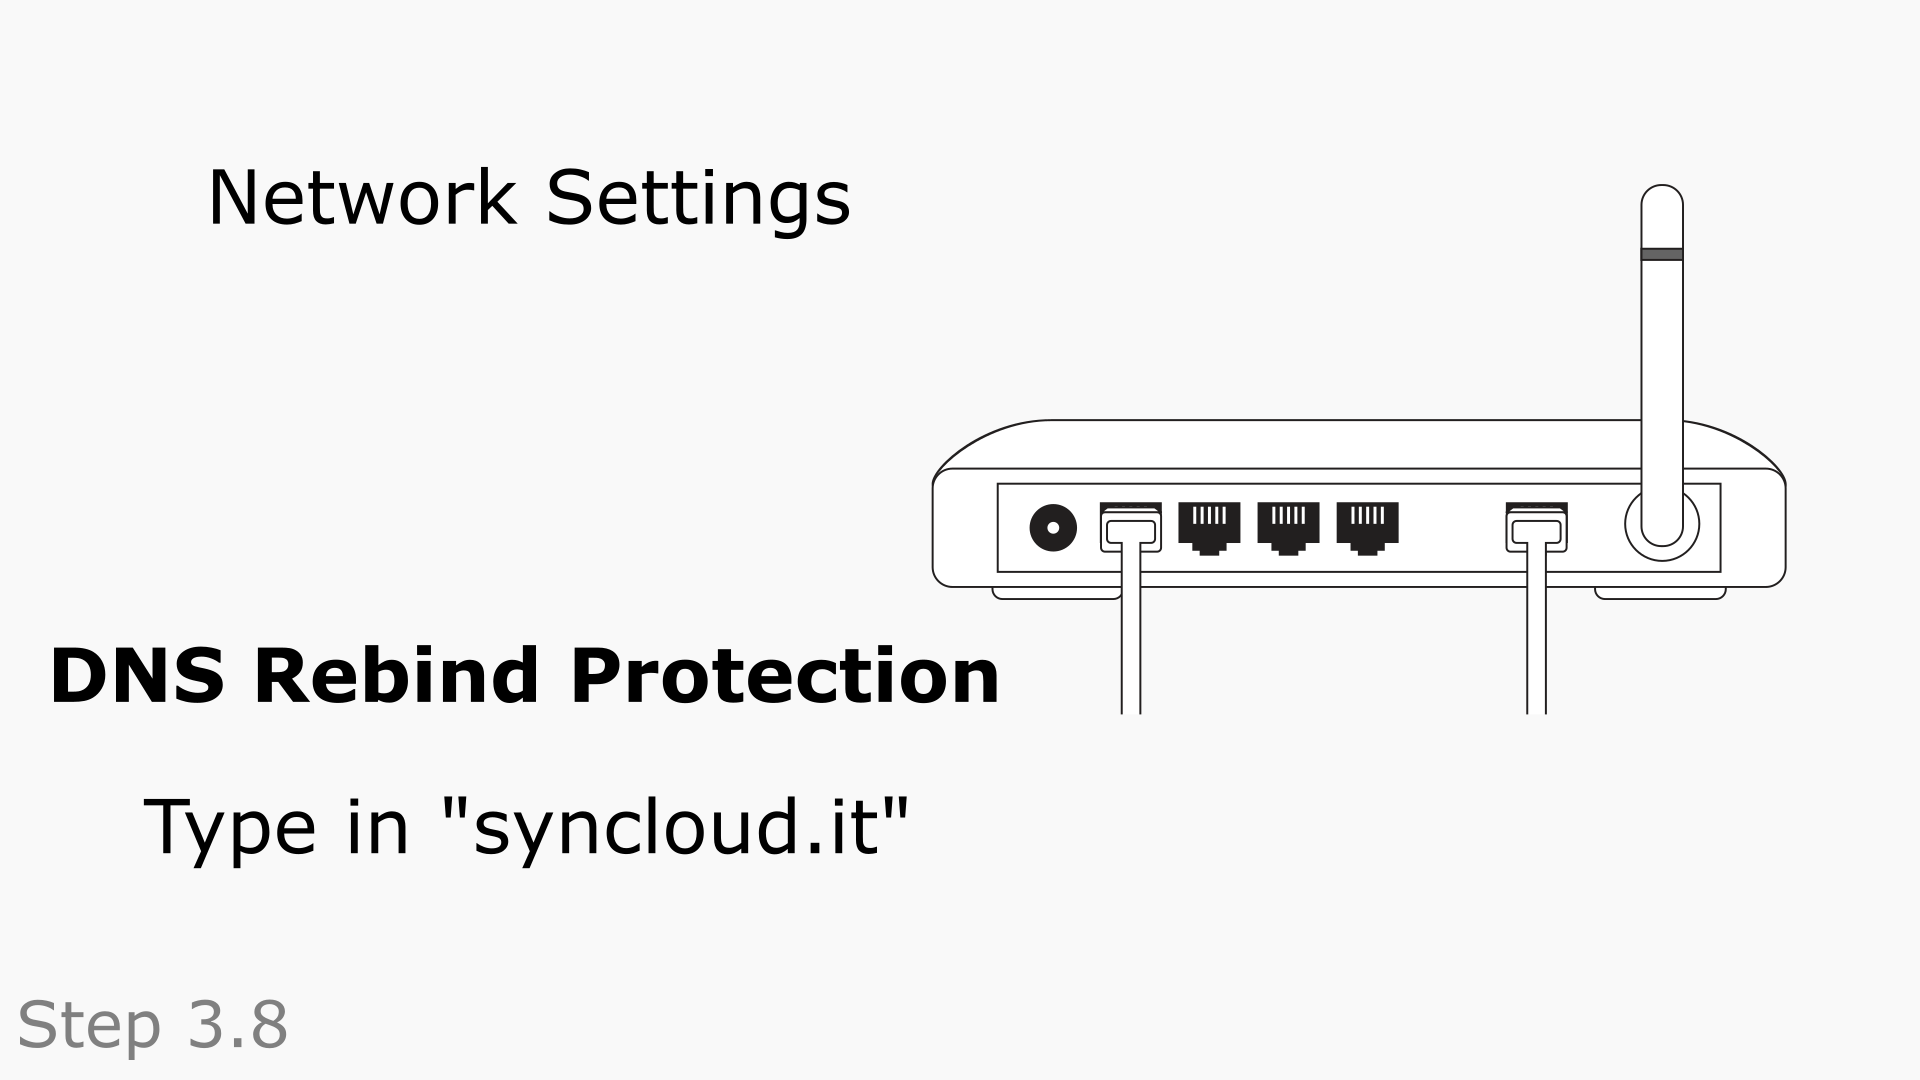
\includegraphics[width=0.7\linewidth]{../frames/37.png}
	\caption{If you can not access the device user interface by your URL, there is probably a so called “DNS rebind protection” in your router settings. Please browse to the web interface of your router and check for DNS rebind protection under your network settings. Add an exception for the domain Syncloud dot it. Now, you should be able to access your device by your URL. If not, please contact our support.}
	\label{fig:25}
\end{figure}

\begin{figure}[htbp!]
	\centering
	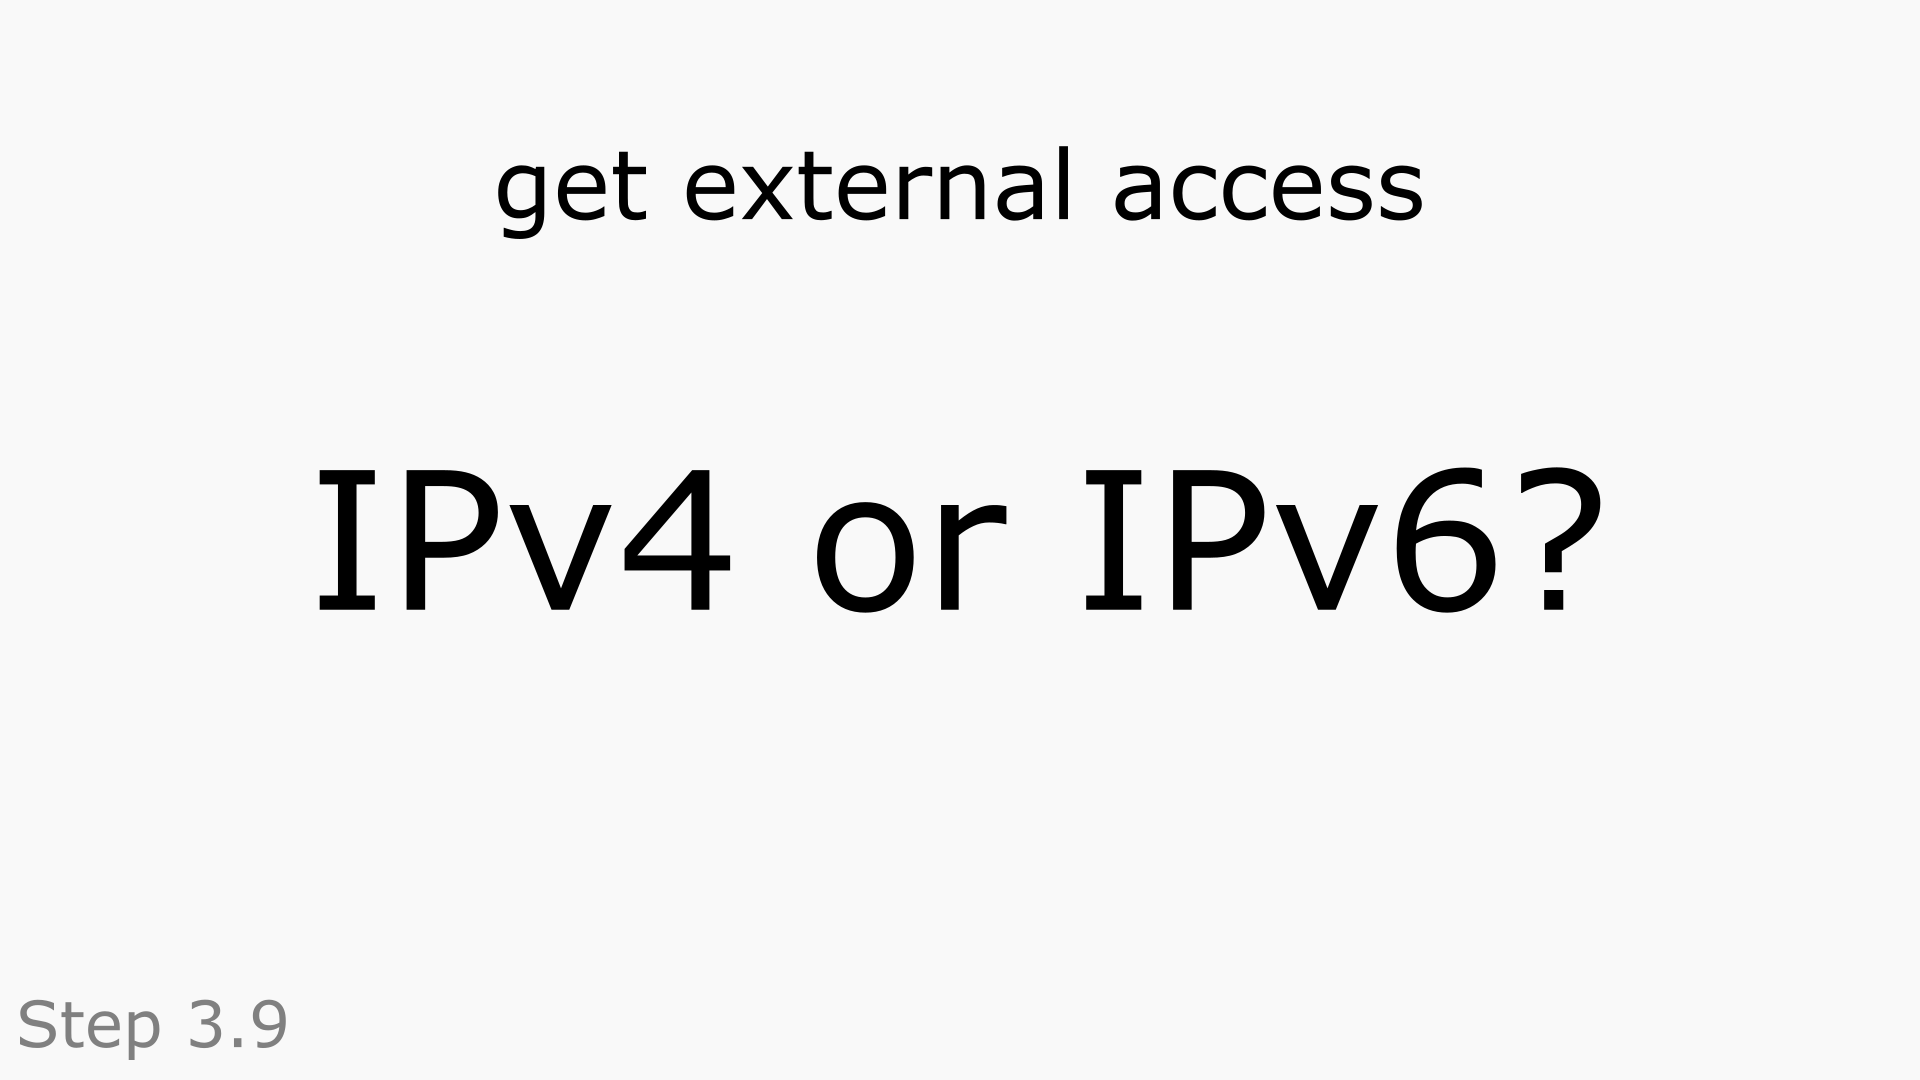
\includegraphics[width=0.7\linewidth]{../frames/38.png}
	\caption{Now, you can make your device accessible from extern, if you want. For that, you must find out if you have version 4 or version 6 of IP address.}
	\label{fig:26}
\end{figure}

\begin{figure}[htbp!]
	\centering
	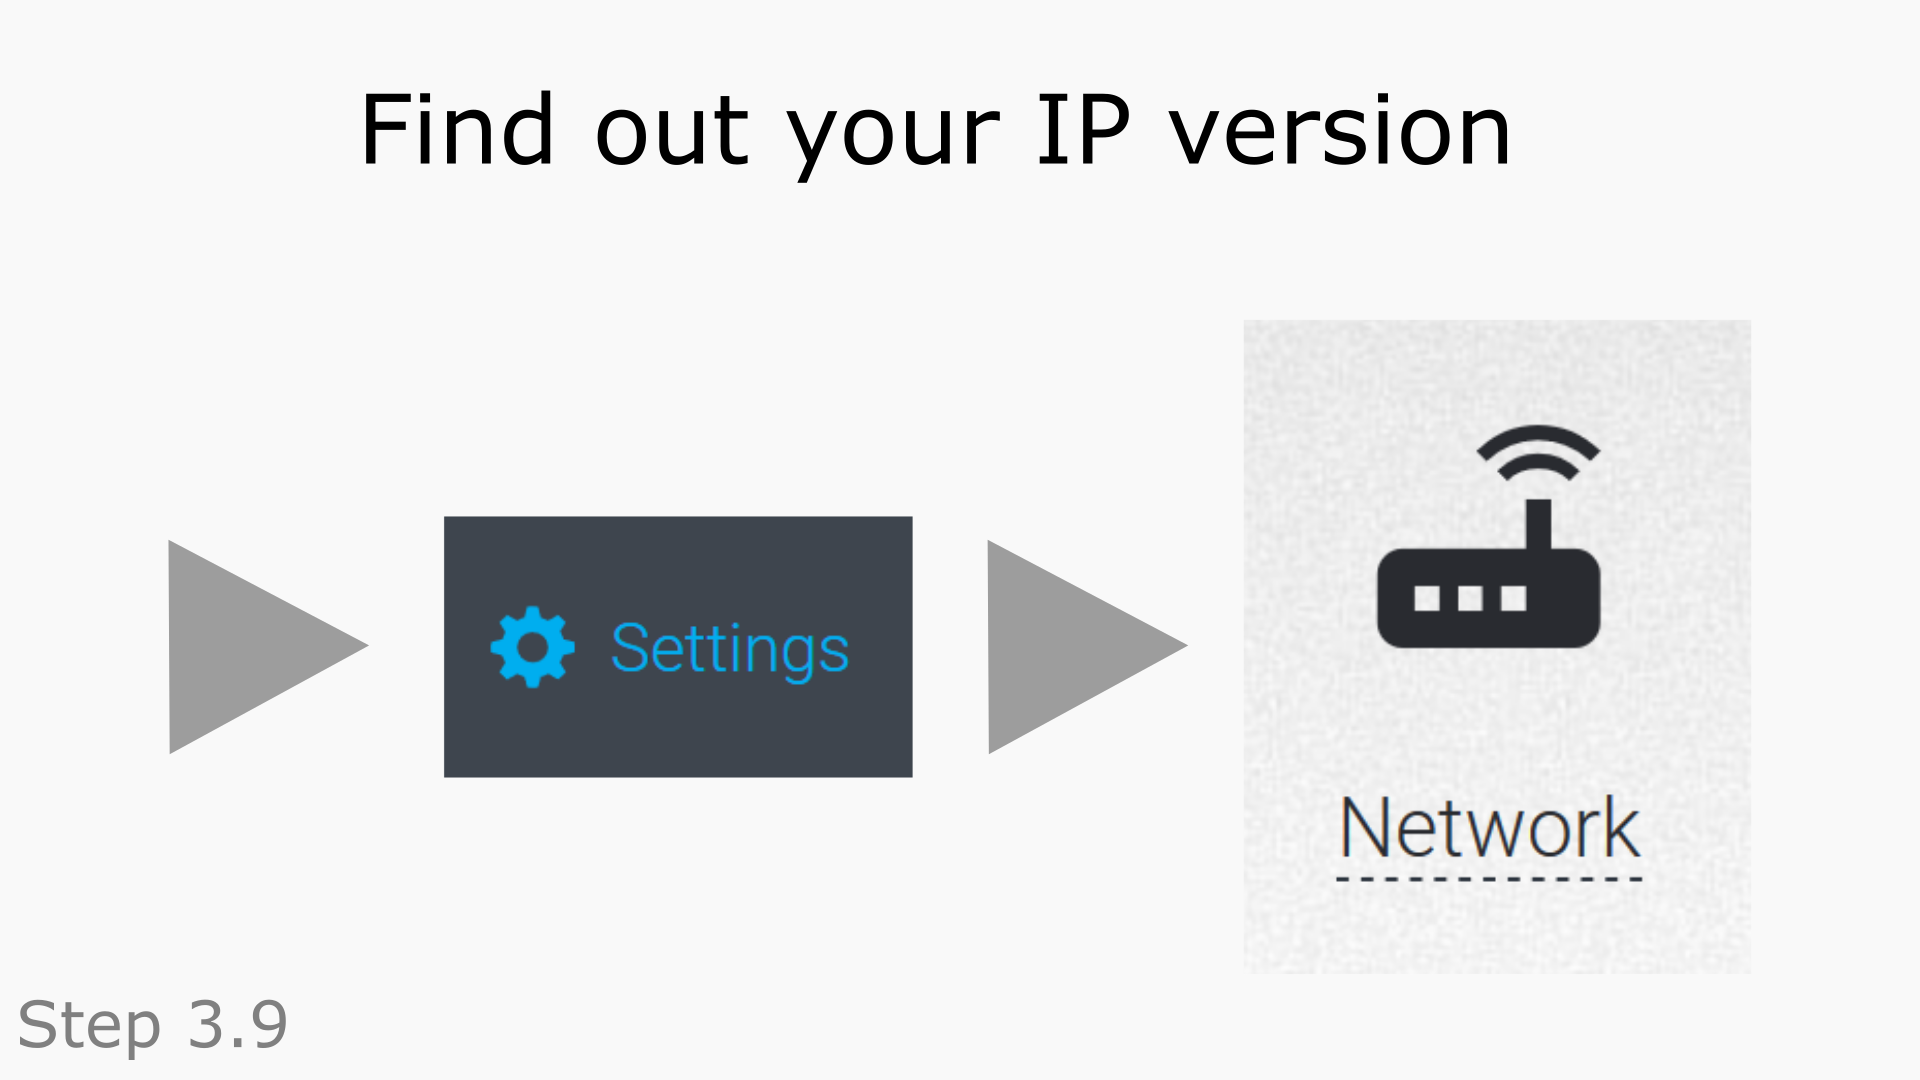
\includegraphics[width=0.7\linewidth]{../frames/39.png}
	\caption{That, you can find out in your device user interface under settings. Click then on Network. If you have IPv6, it will appear with the IP address of your device.}
	\label{fig:27}
\end{figure}

\begin{figure}[htbp!]
	\centering
	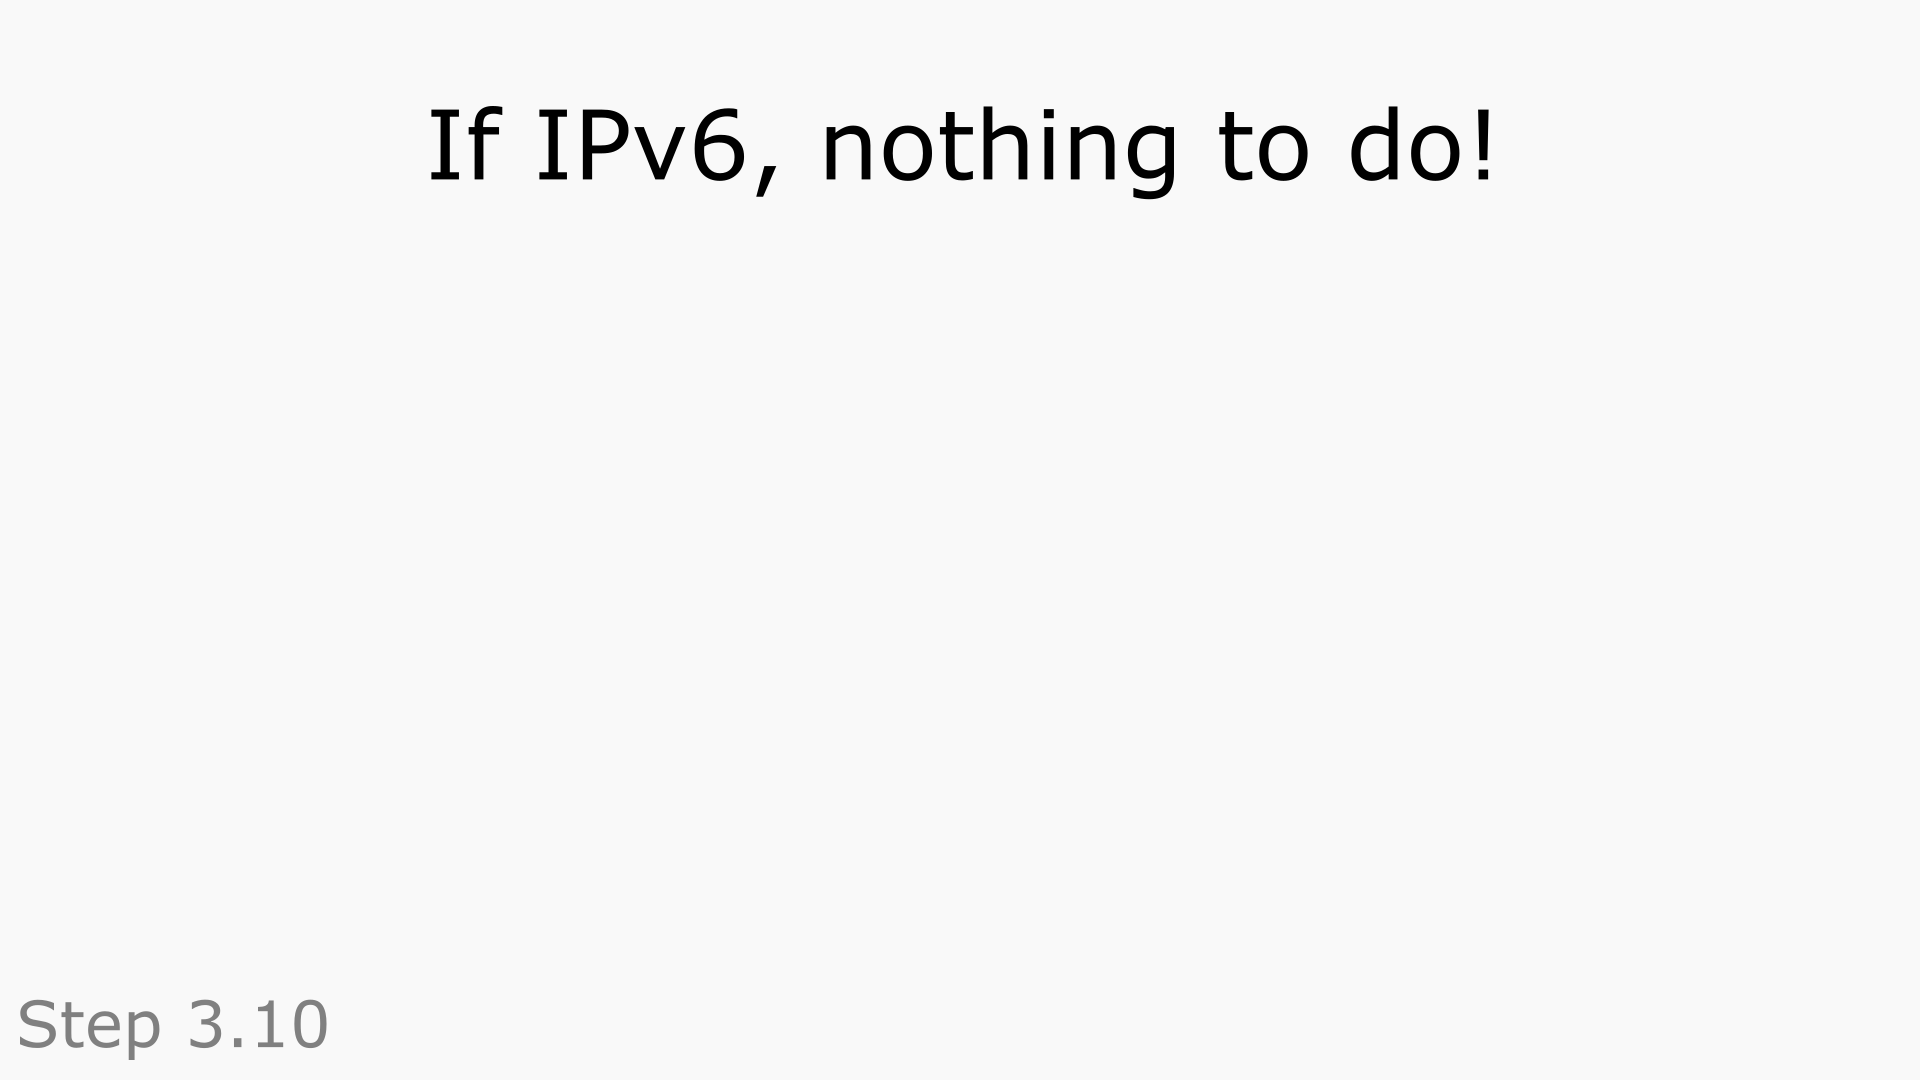
\includegraphics[width=0.7\linewidth]{../frames/40.png}
	\caption{With IPv6 you can access your device from extern by default, so you don’t have to activate external access in the device settings. However, you must know, that you can only access from an IPv6 network and that you cannot access from an IPv4 network. Sadly, many public networks like of companies or schools and many mobile networks do not have IPv6 support.}
	\label{fig:28}
\end{figure}

\begin{figure}[htbp!]
	\centering
	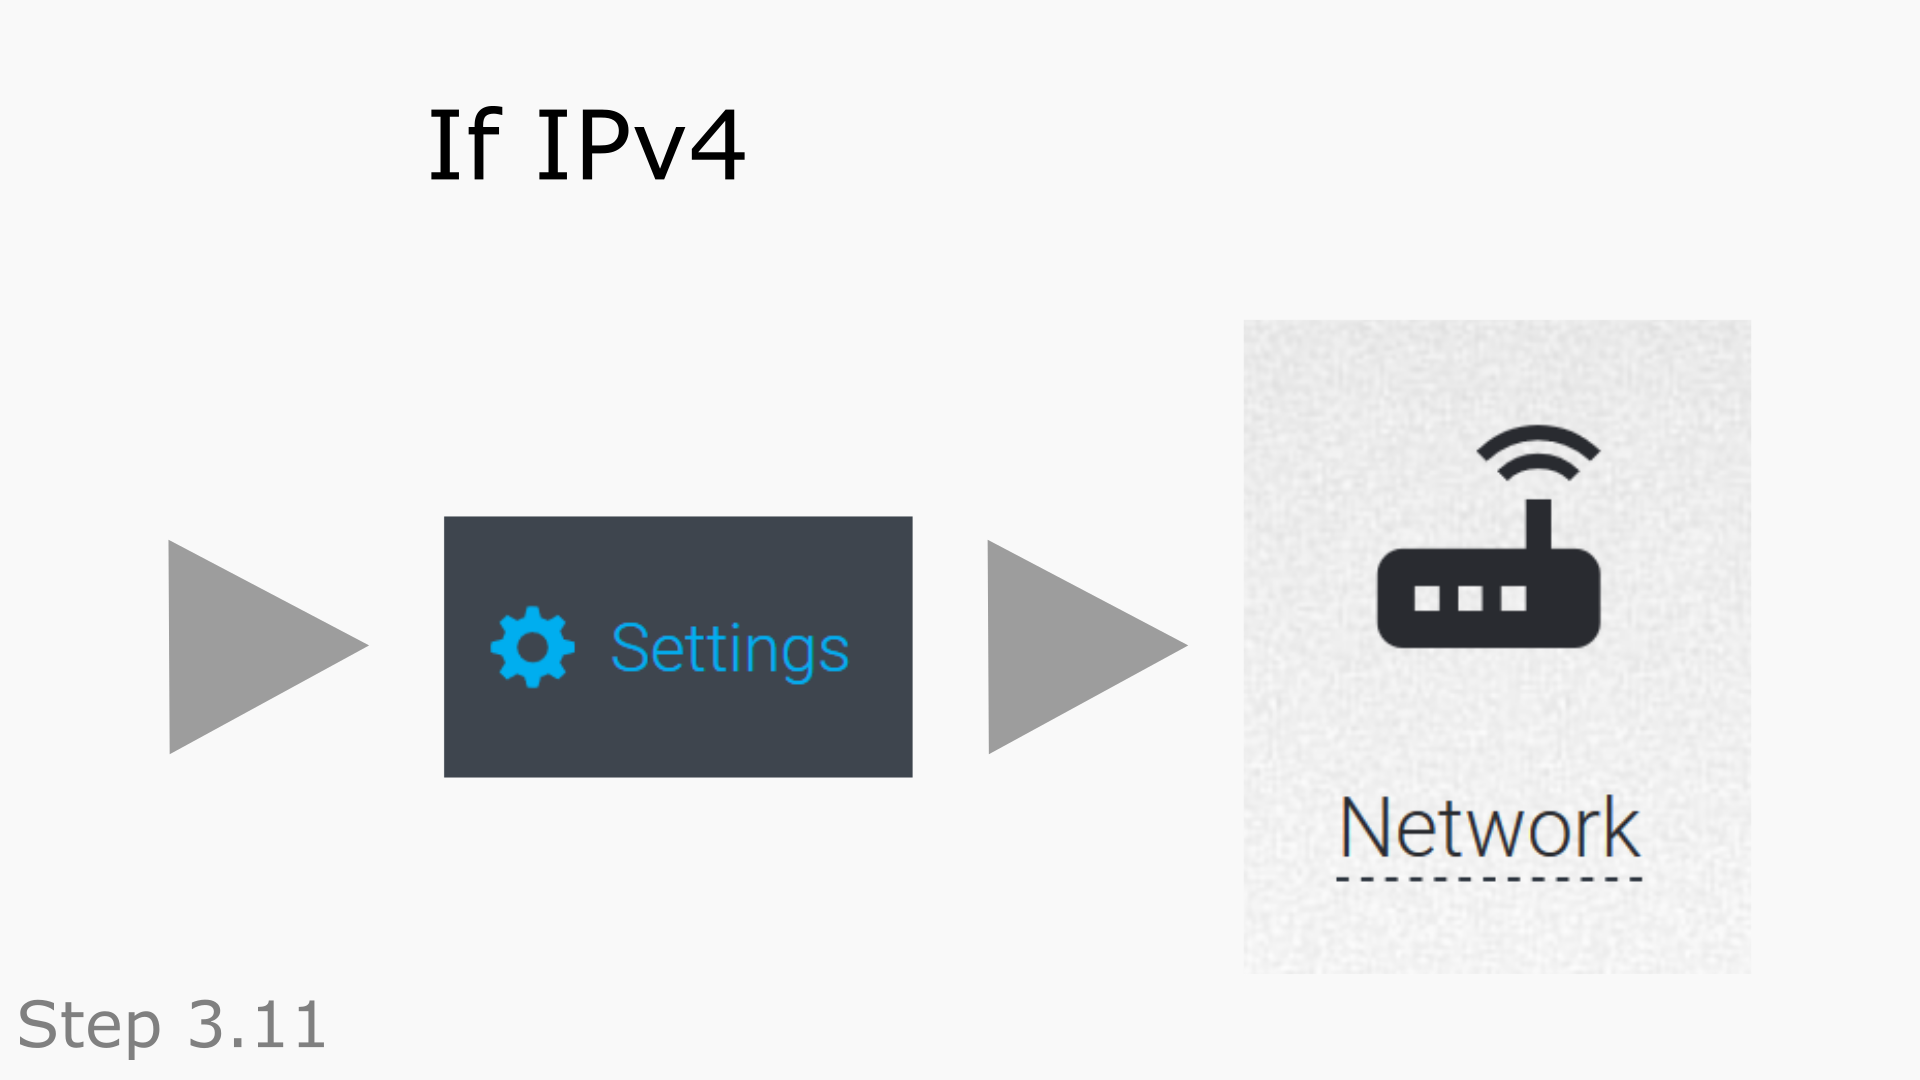
\includegraphics[width=0.7\linewidth]{../frames/41.png}
	\caption{If you have IPv4, you must enable external access in your device settings. You must open two ports in your router called 80 and 443. You can try to do this with auto mode and save. Sometimes it fails. However, there is no reason to worry.}
	\label{fig:29}
\end{figure}

\begin{figure}[htbp!]
	\centering
	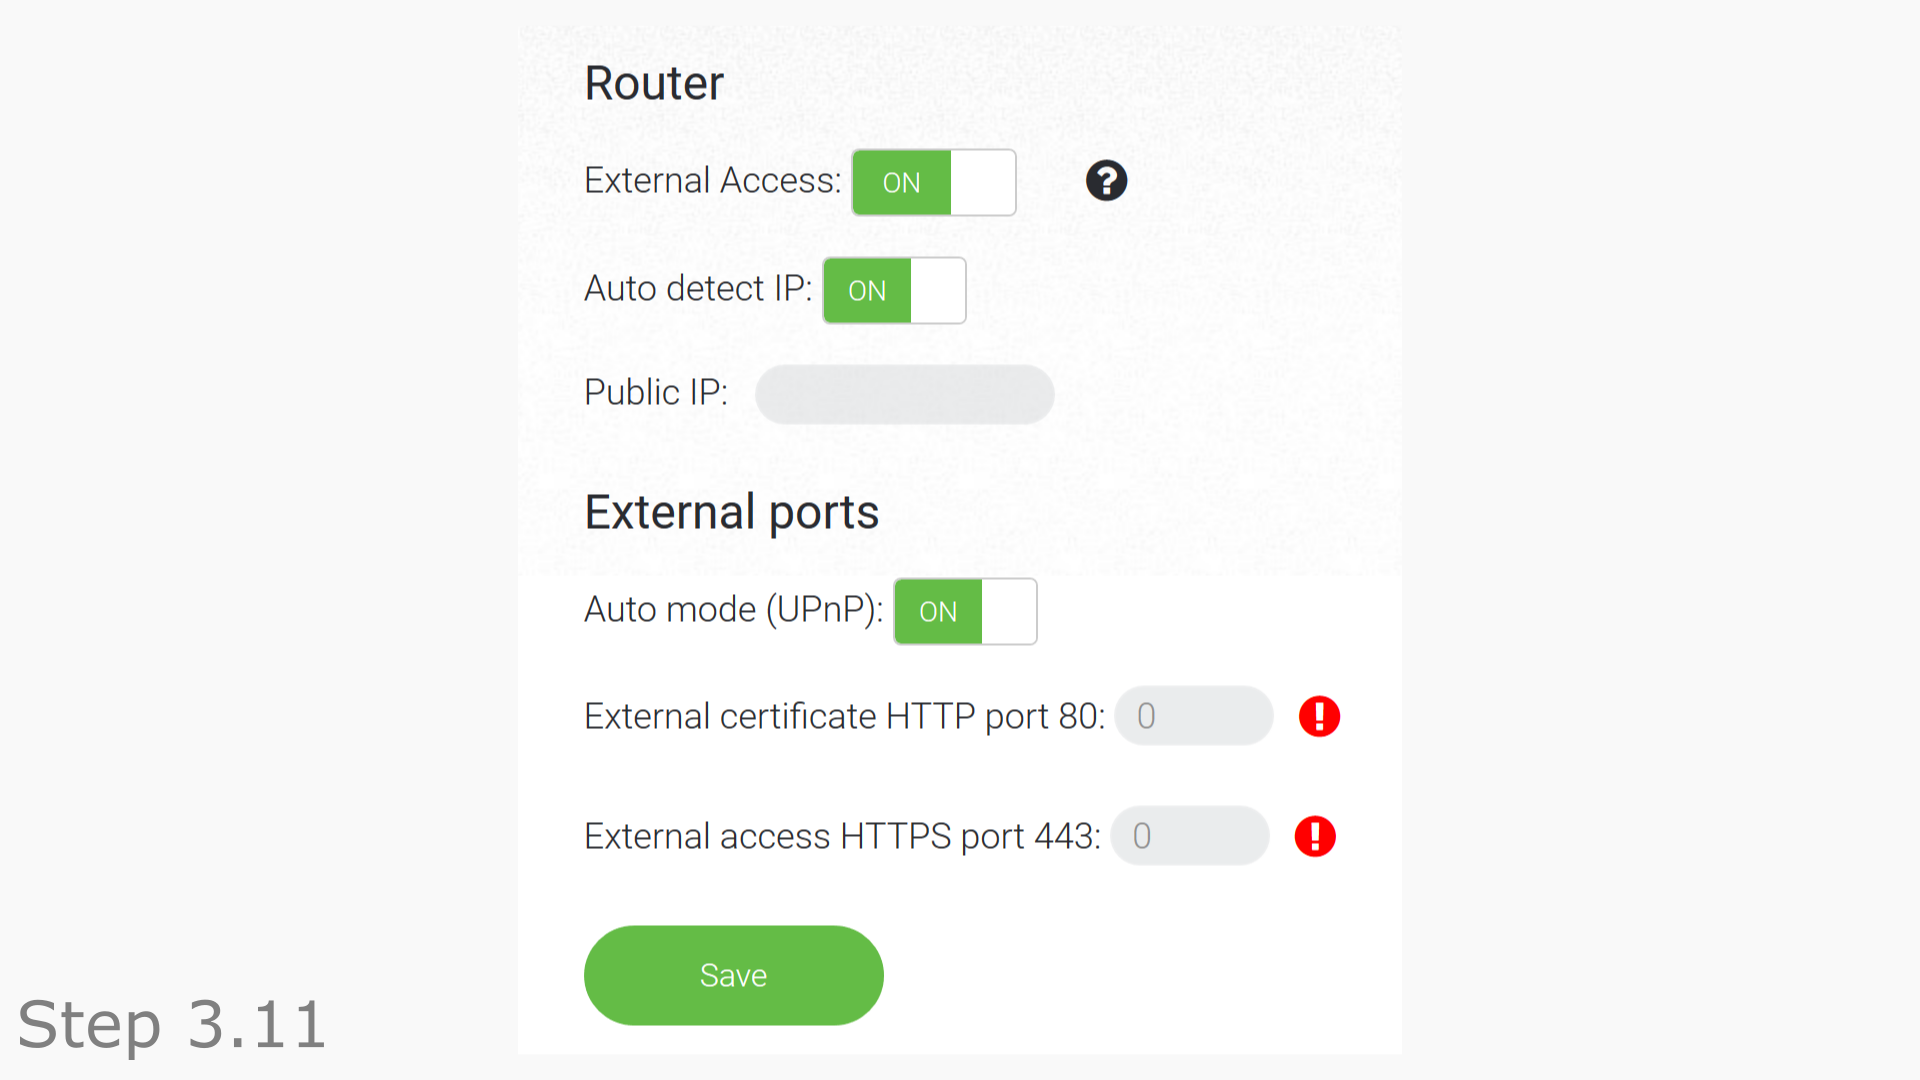
\includegraphics[width=0.7\linewidth]{../frames/43.png}
	\caption{see above}
	\label{fig:30}
\end{figure}

\begin{figure}[htbp!]
	\centering
	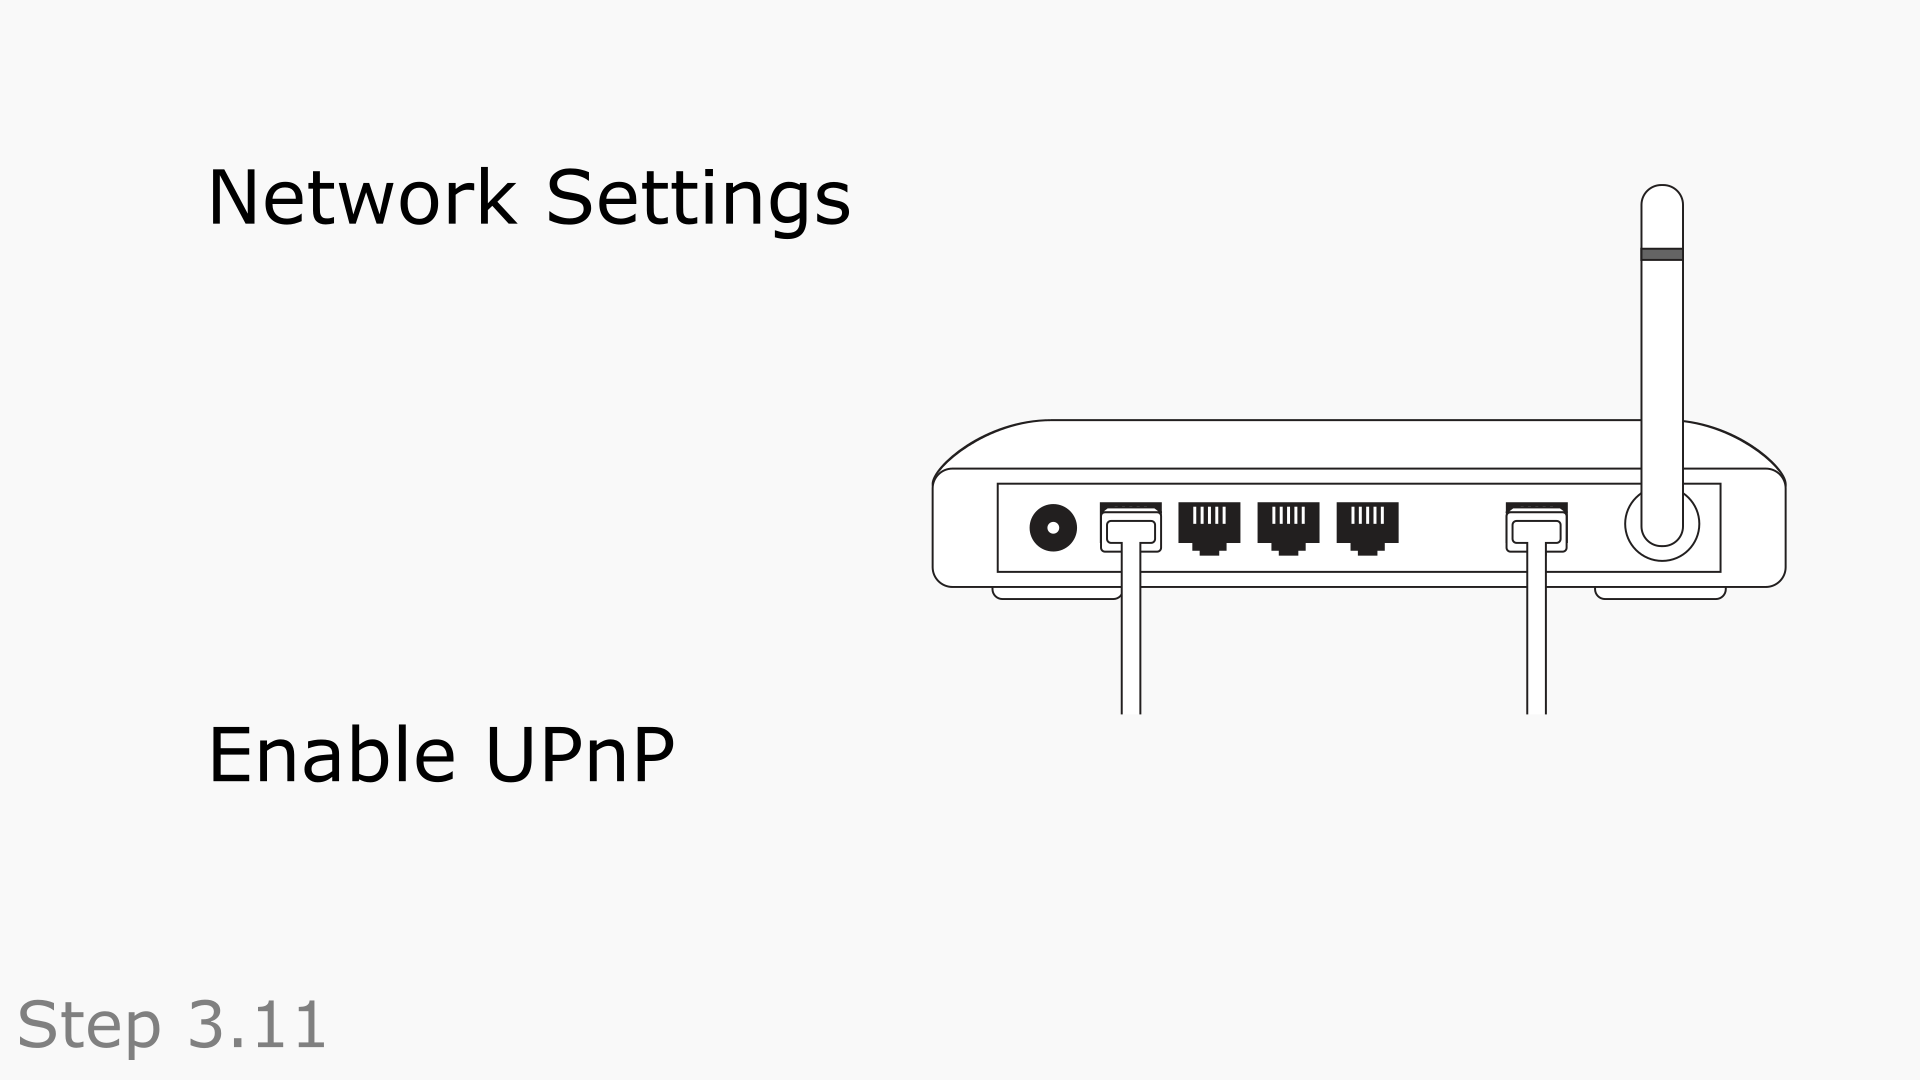
\includegraphics[width=0.7\linewidth]{../frames/44.png}
	\caption{You probably must enable UPnP in your router settings. Then try it again.}
	\label{fig:31}
\end{figure}

\begin{figure}[htbp!]
	\centering
	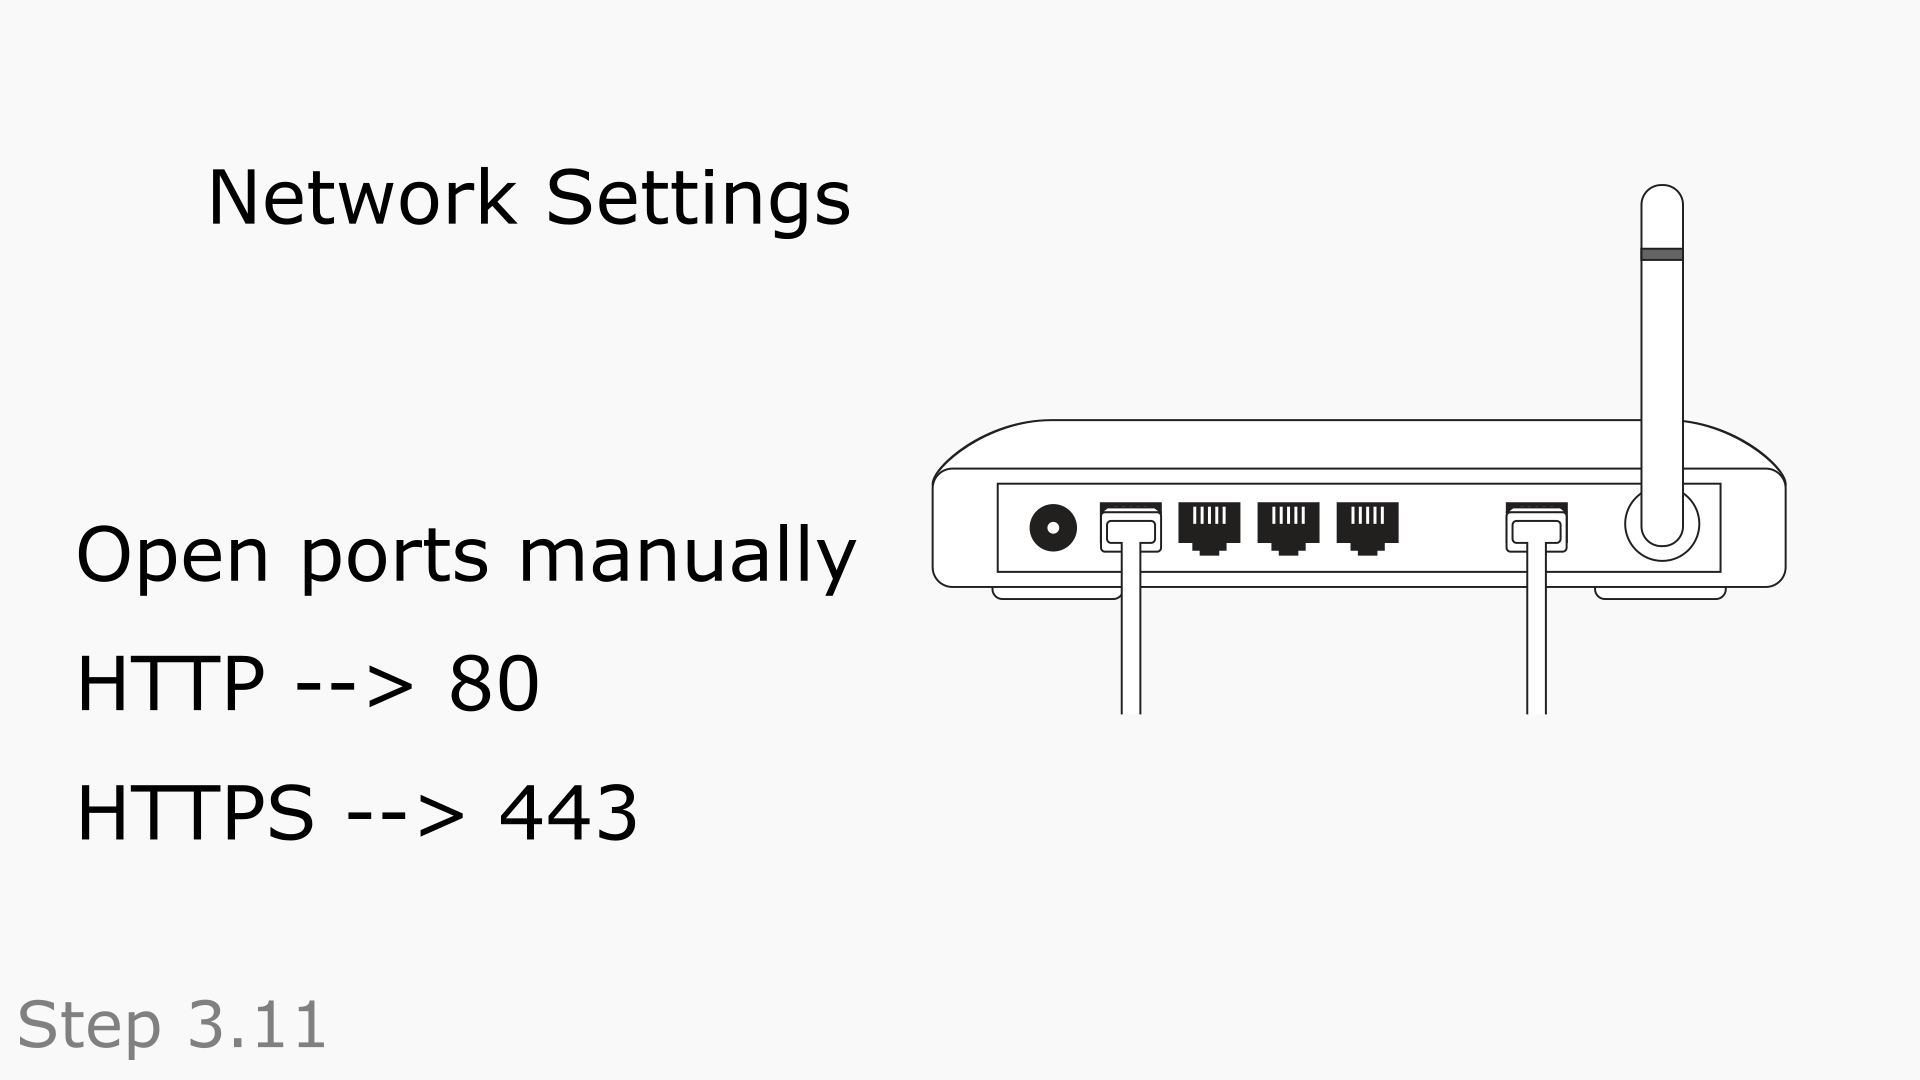
\includegraphics[width=0.7\linewidth]{../frames/45.png}
	\caption{If it fails again, you must open the two ports manually in your router settings. Open 80 for HTTP and 443 for HTTPS.}
	\label{fig:32}
\end{figure}

\begin{figure}[htbp!]
	\centering
	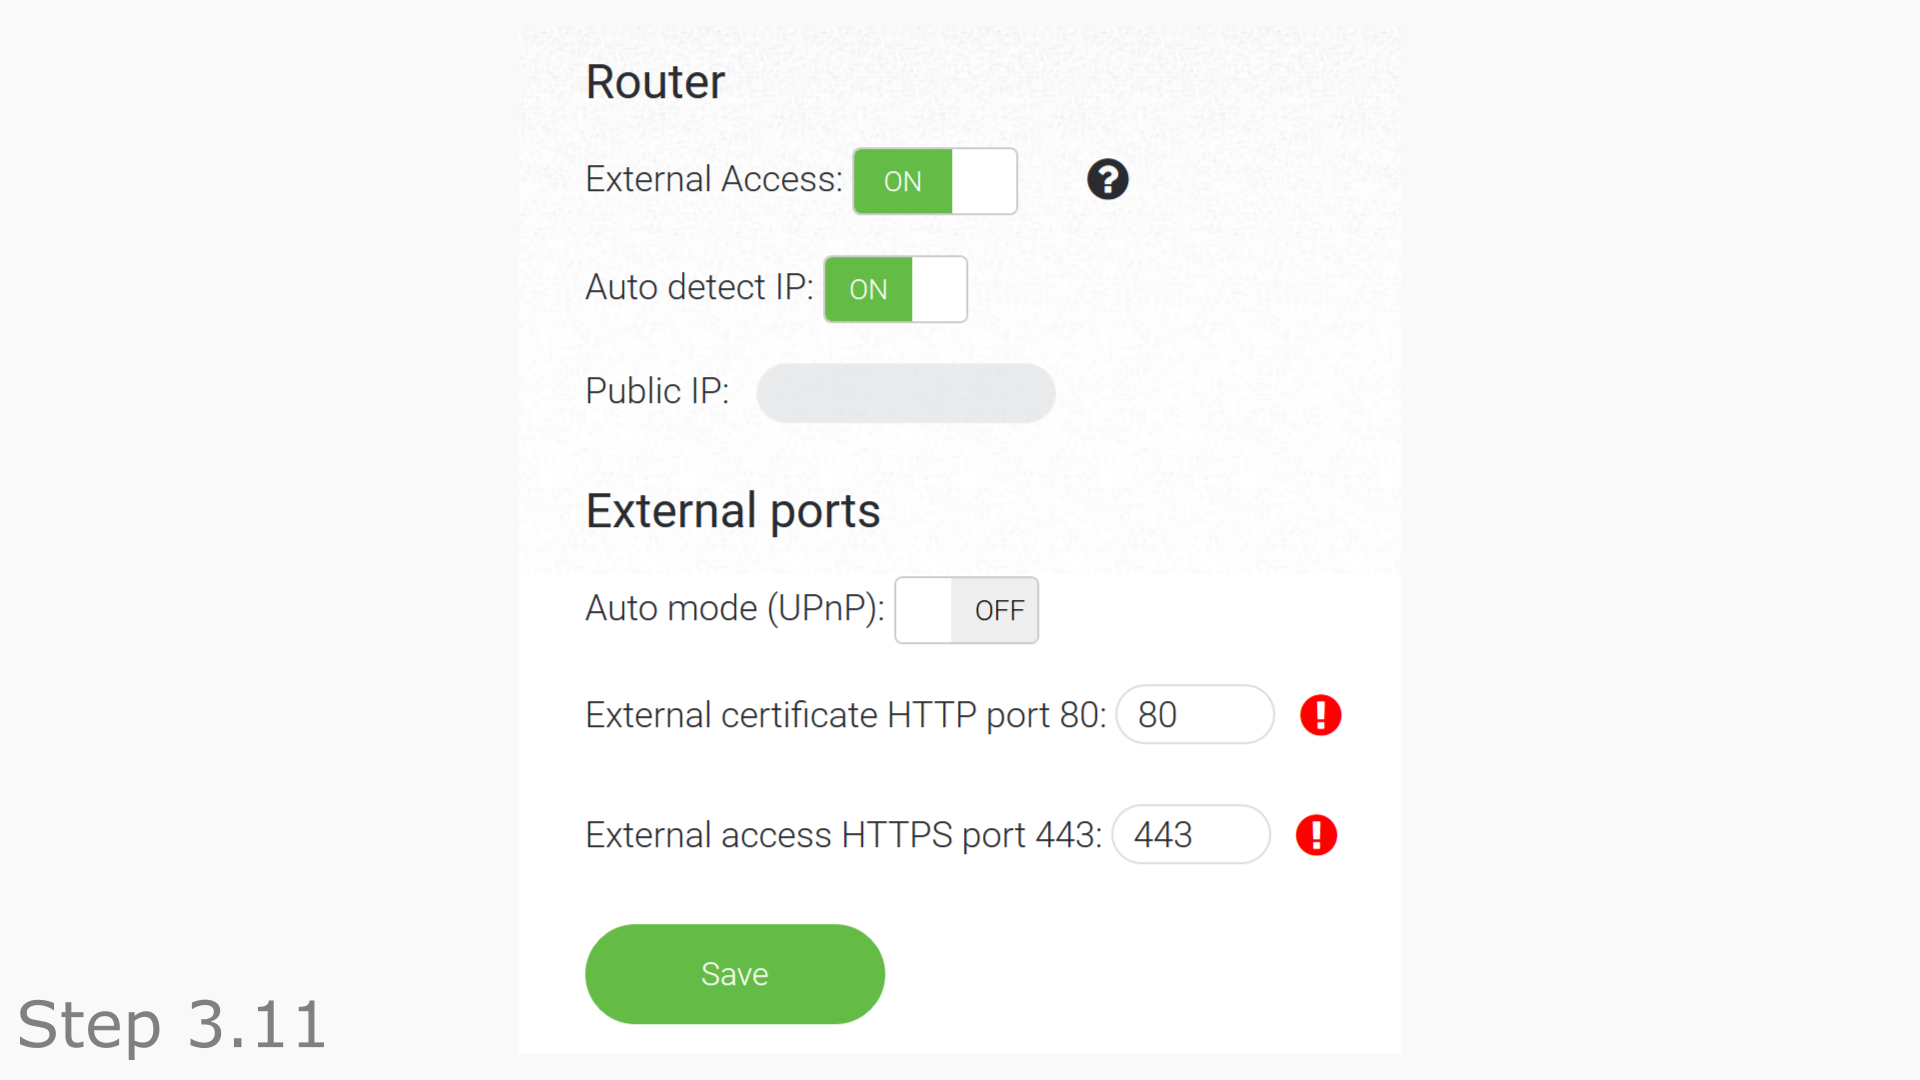
\includegraphics[width=0.7\linewidth]{../frames/46.png}
	\caption{Then, type 80 and 443 in the input fields in the device user interface and save. Now, you should be able to enable external access. If not, please contact our support.}
	\label{fig:33}
\end{figure}

\section{Now you are ready!}

\begin{figure}[htbp!]
	\centering
	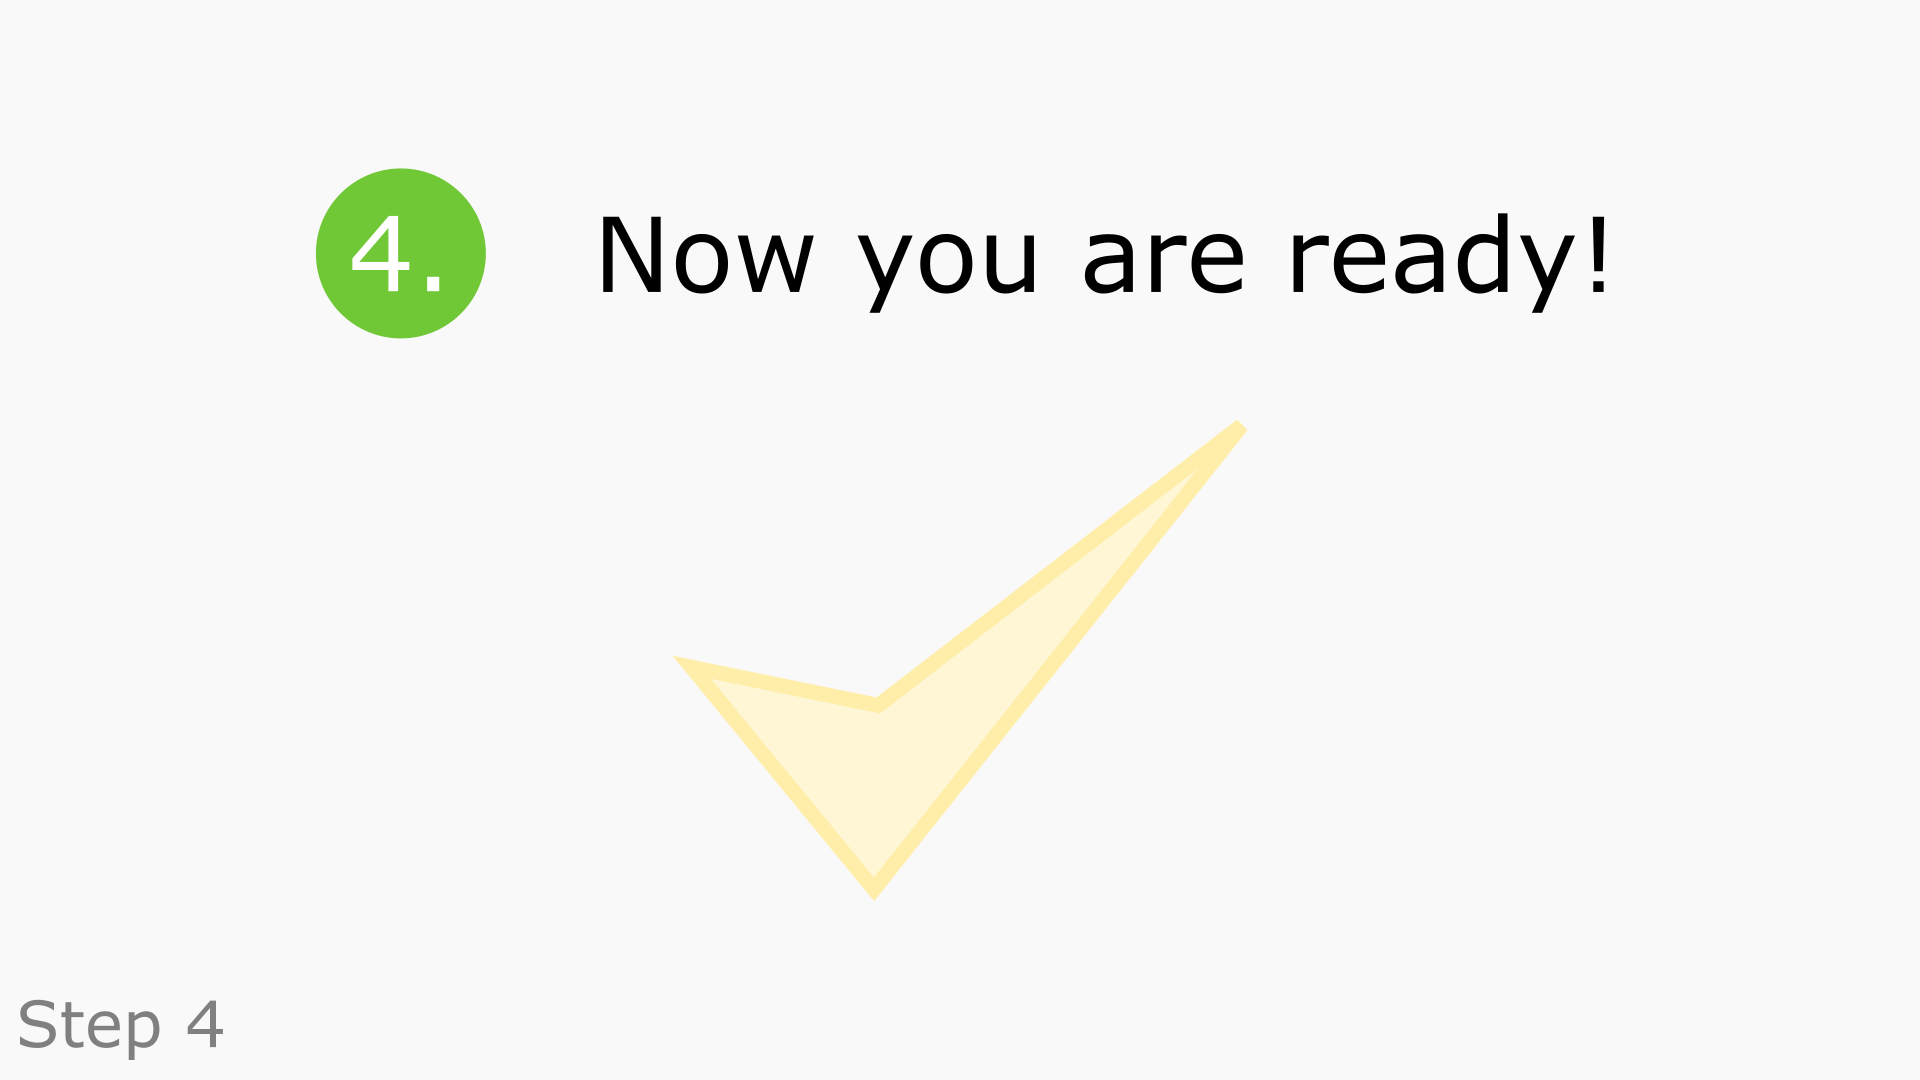
\includegraphics[width=0.7\linewidth]{../frames/47.png}
	\caption{Now, you are ready to discover and enjoy your new device.}
	\label{fig:34}
\end{figure}

\begin{figure}[htbp!]
	\centering
	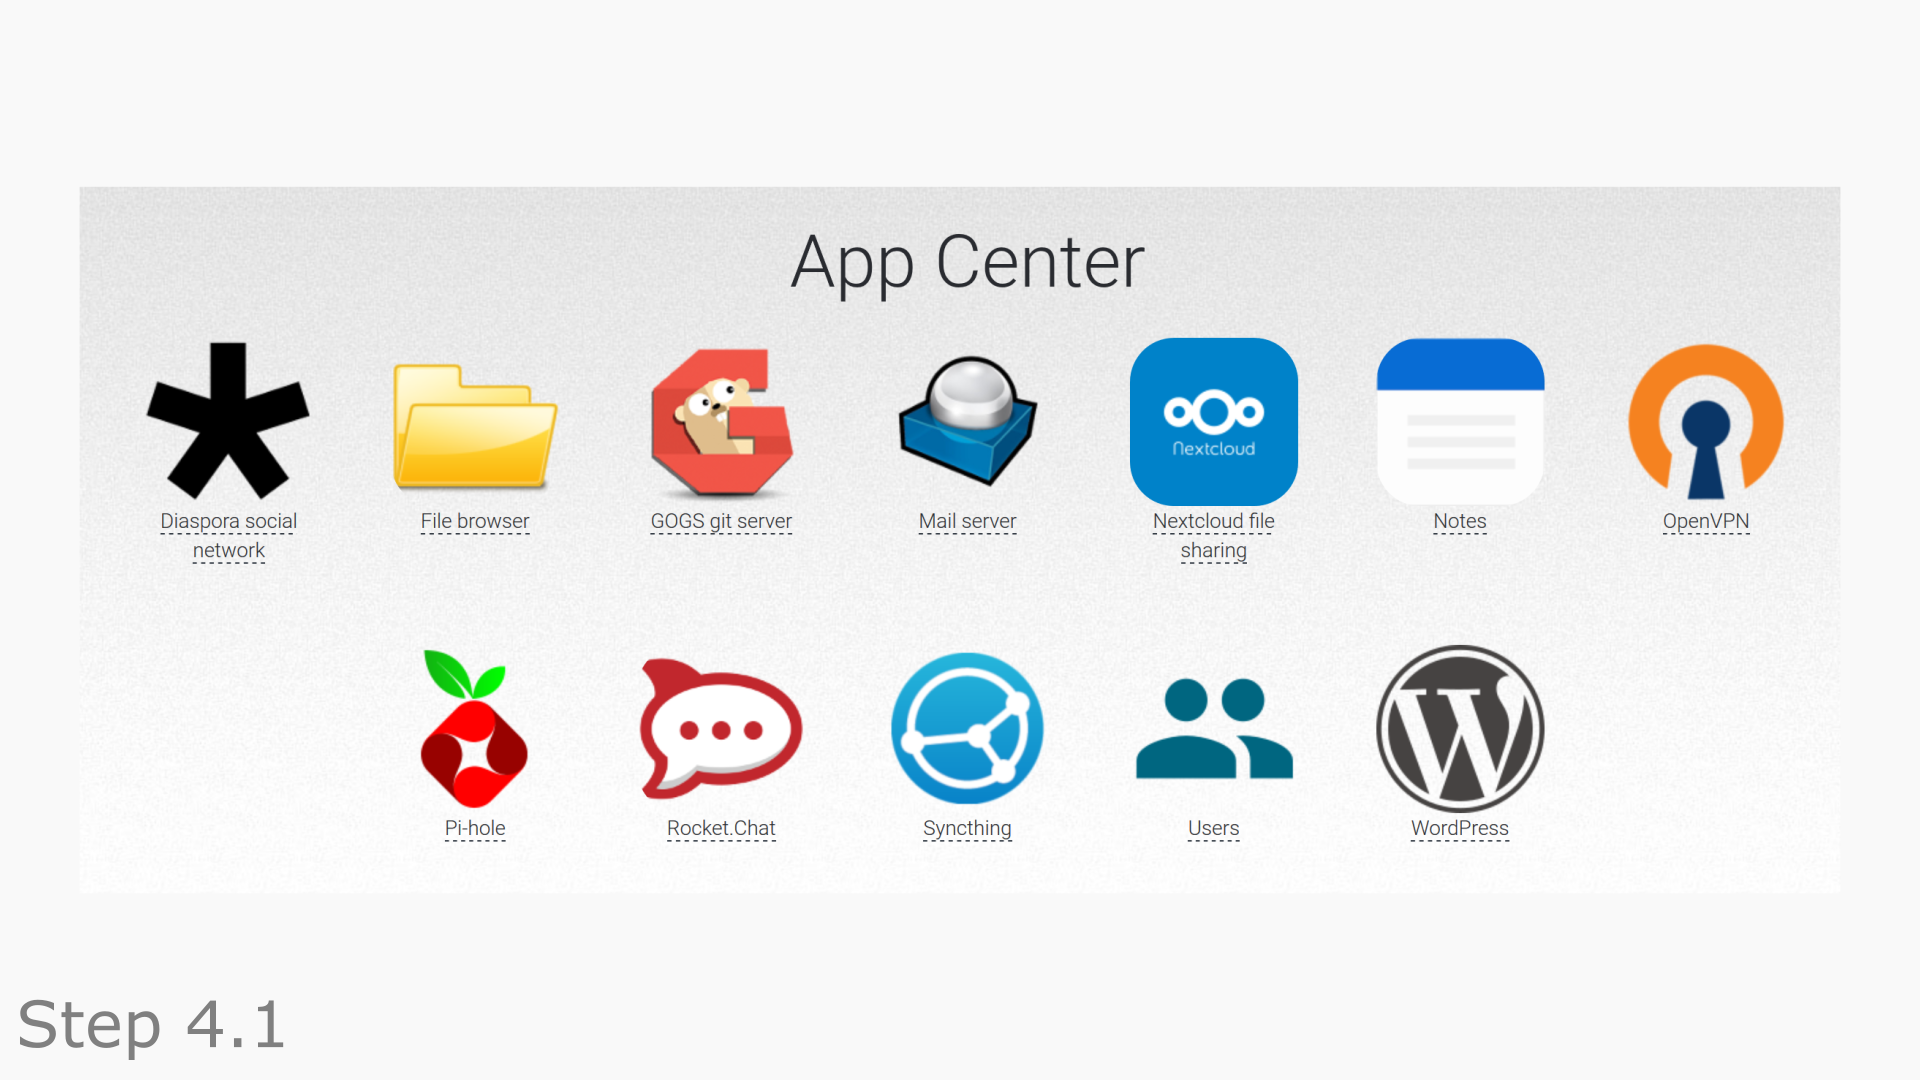
\includegraphics[width=0.7\linewidth]{../frames/48.png}
	\caption{Go to our app center to install an app. Click on any app, for example Nextcloud.}
	\label{fig:35}
\end{figure}

\begin{figure}[htbp!]
	\centering
	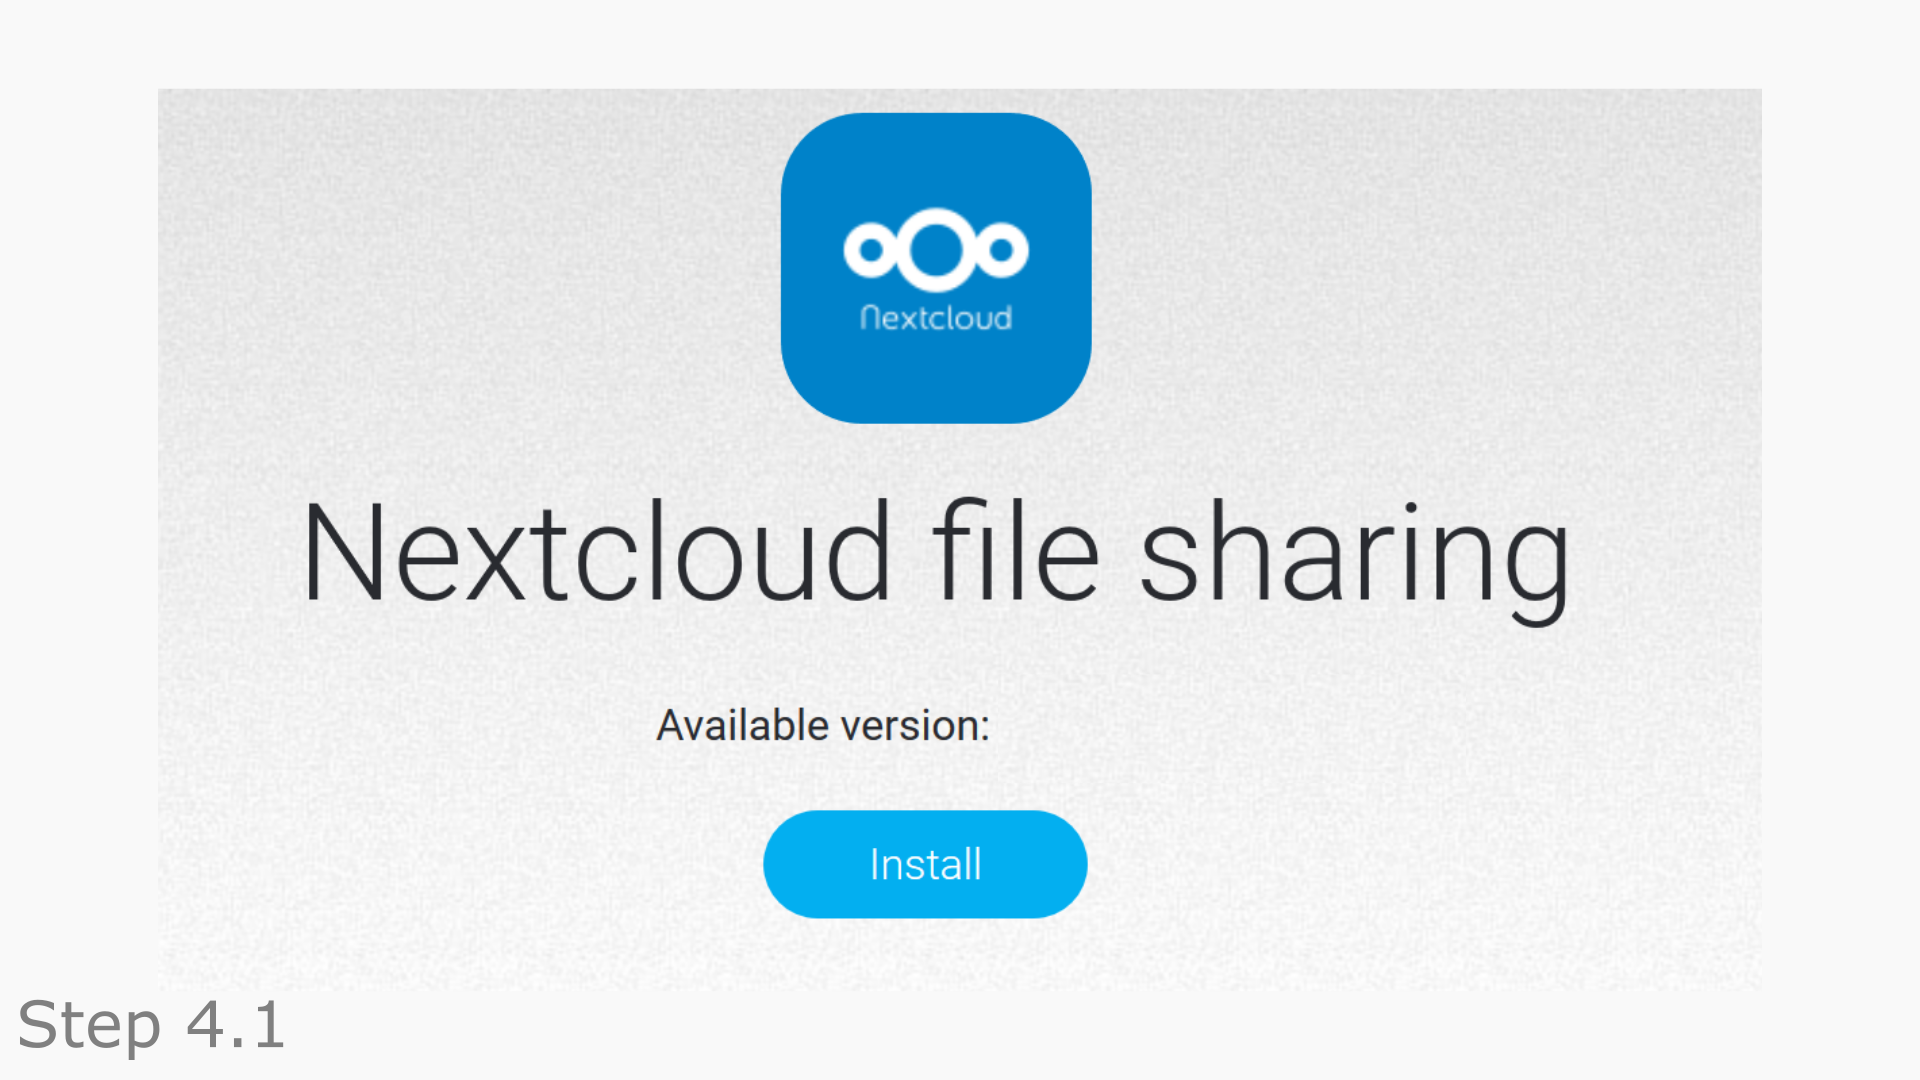
\includegraphics[width=0.7\linewidth]{../frames/49.png}
	\caption{Click on Install and wait untill the Open button appears.}
	\label{fig:36}
\end{figure}

\begin{figure}[htbp!]
	\centering
	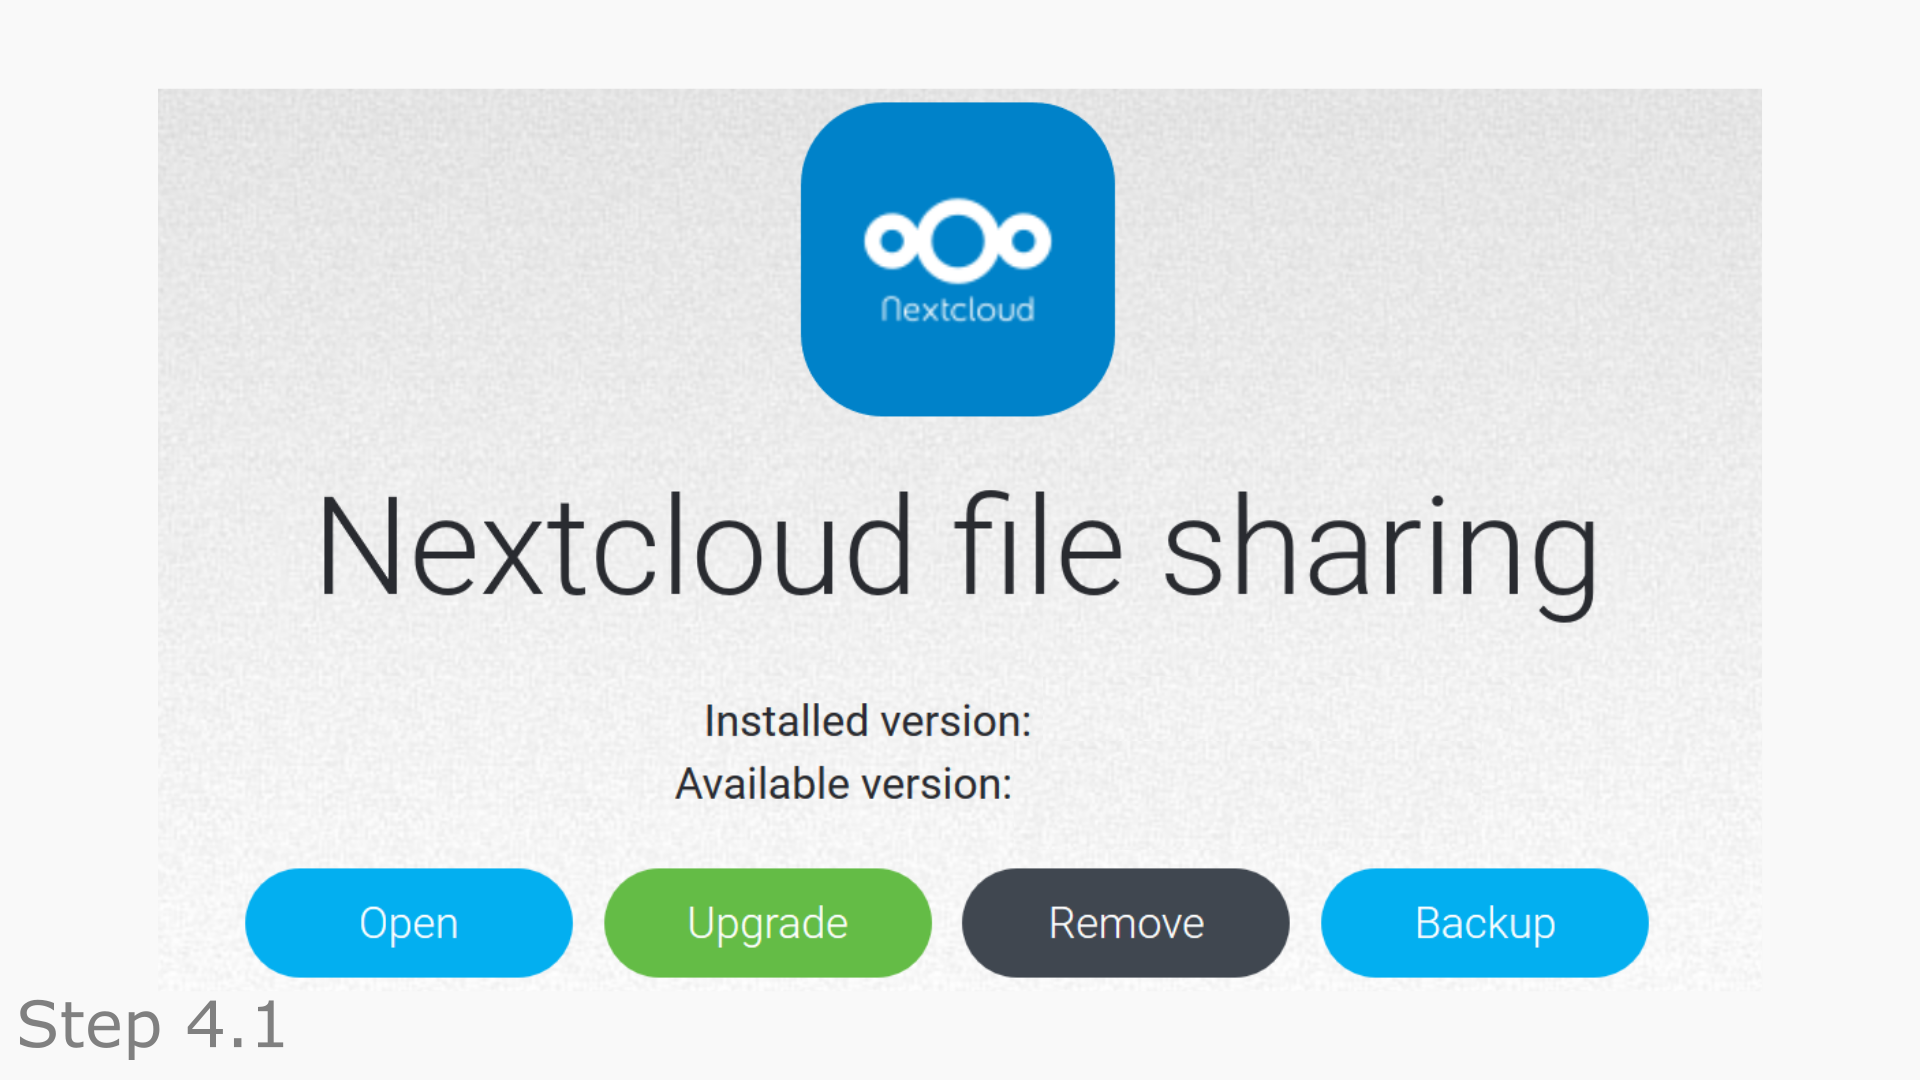
\includegraphics[width=0.7\linewidth]{../frames/50.png}
	\caption{Enjoy your new app. Besides that, you can upgrade, backup or remove the app.}
	\label{fig:37}
\end{figure}

\begin{figure}[htbp!]
	\centering
	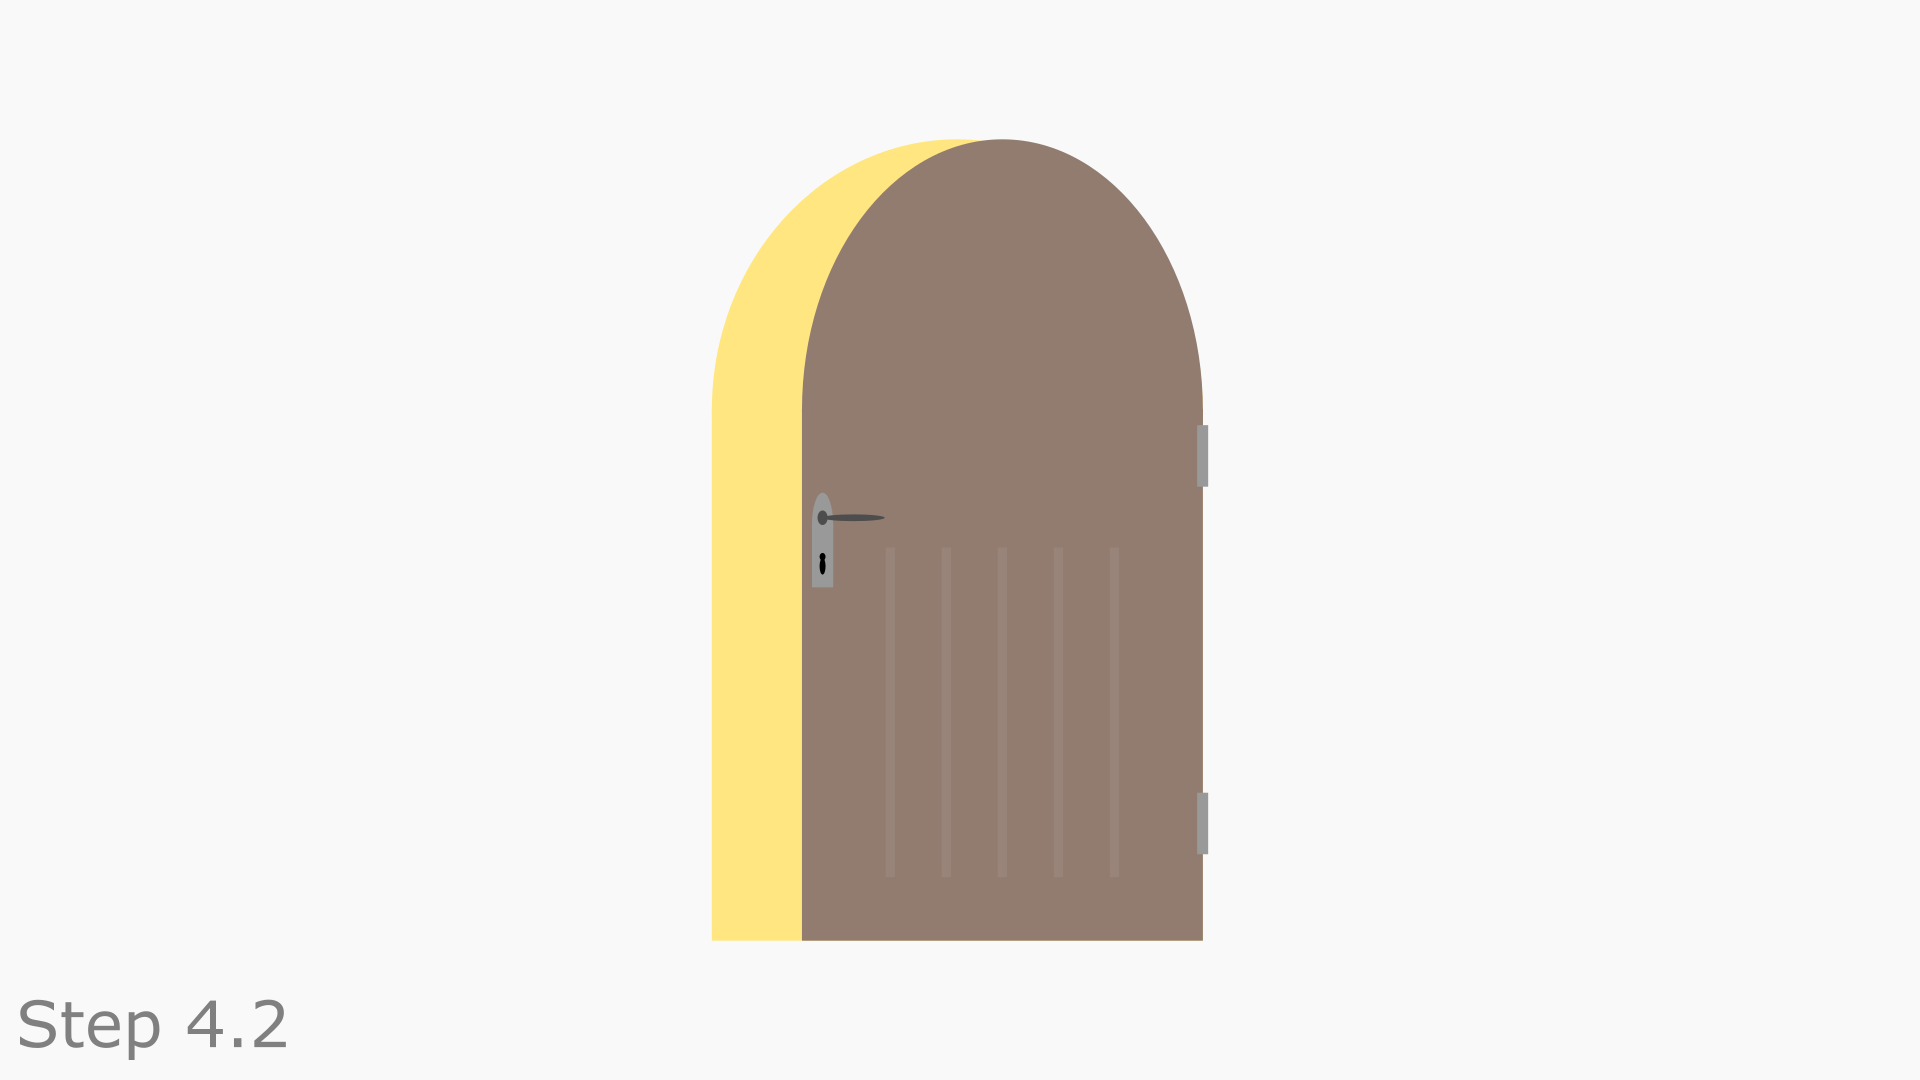
\includegraphics[width=0.7\linewidth]{../frames/51.png}
	\caption{For some apps, you have to open ports in your router.}
	\label{fig:38}
\end{figure}

\begin{figure}[htbp!]
	\centering
	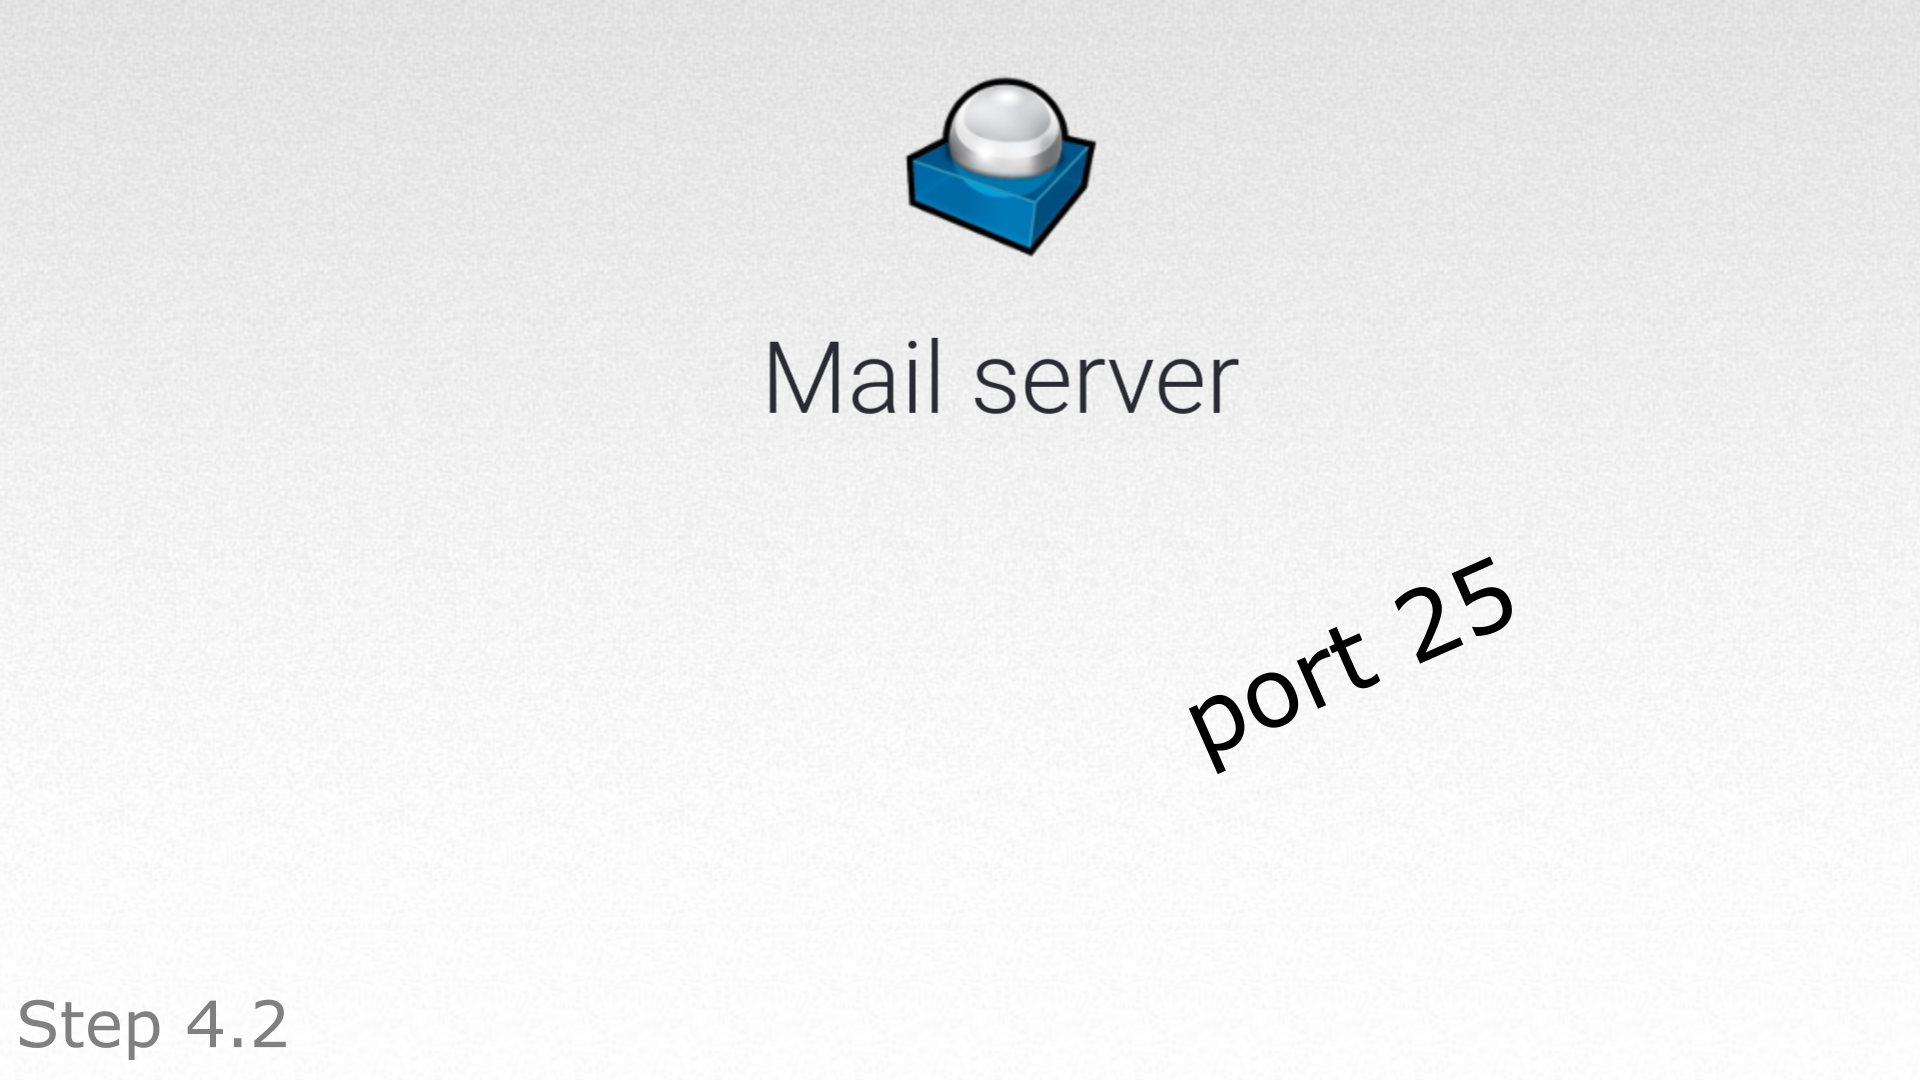
\includegraphics[width=0.7\linewidth]{../frames/52.png}
	\caption{For example, the Mail server app needs open port 25.}
	\label{fig:39}
\end{figure}

\begin{figure}[htbp!]
	\centering
	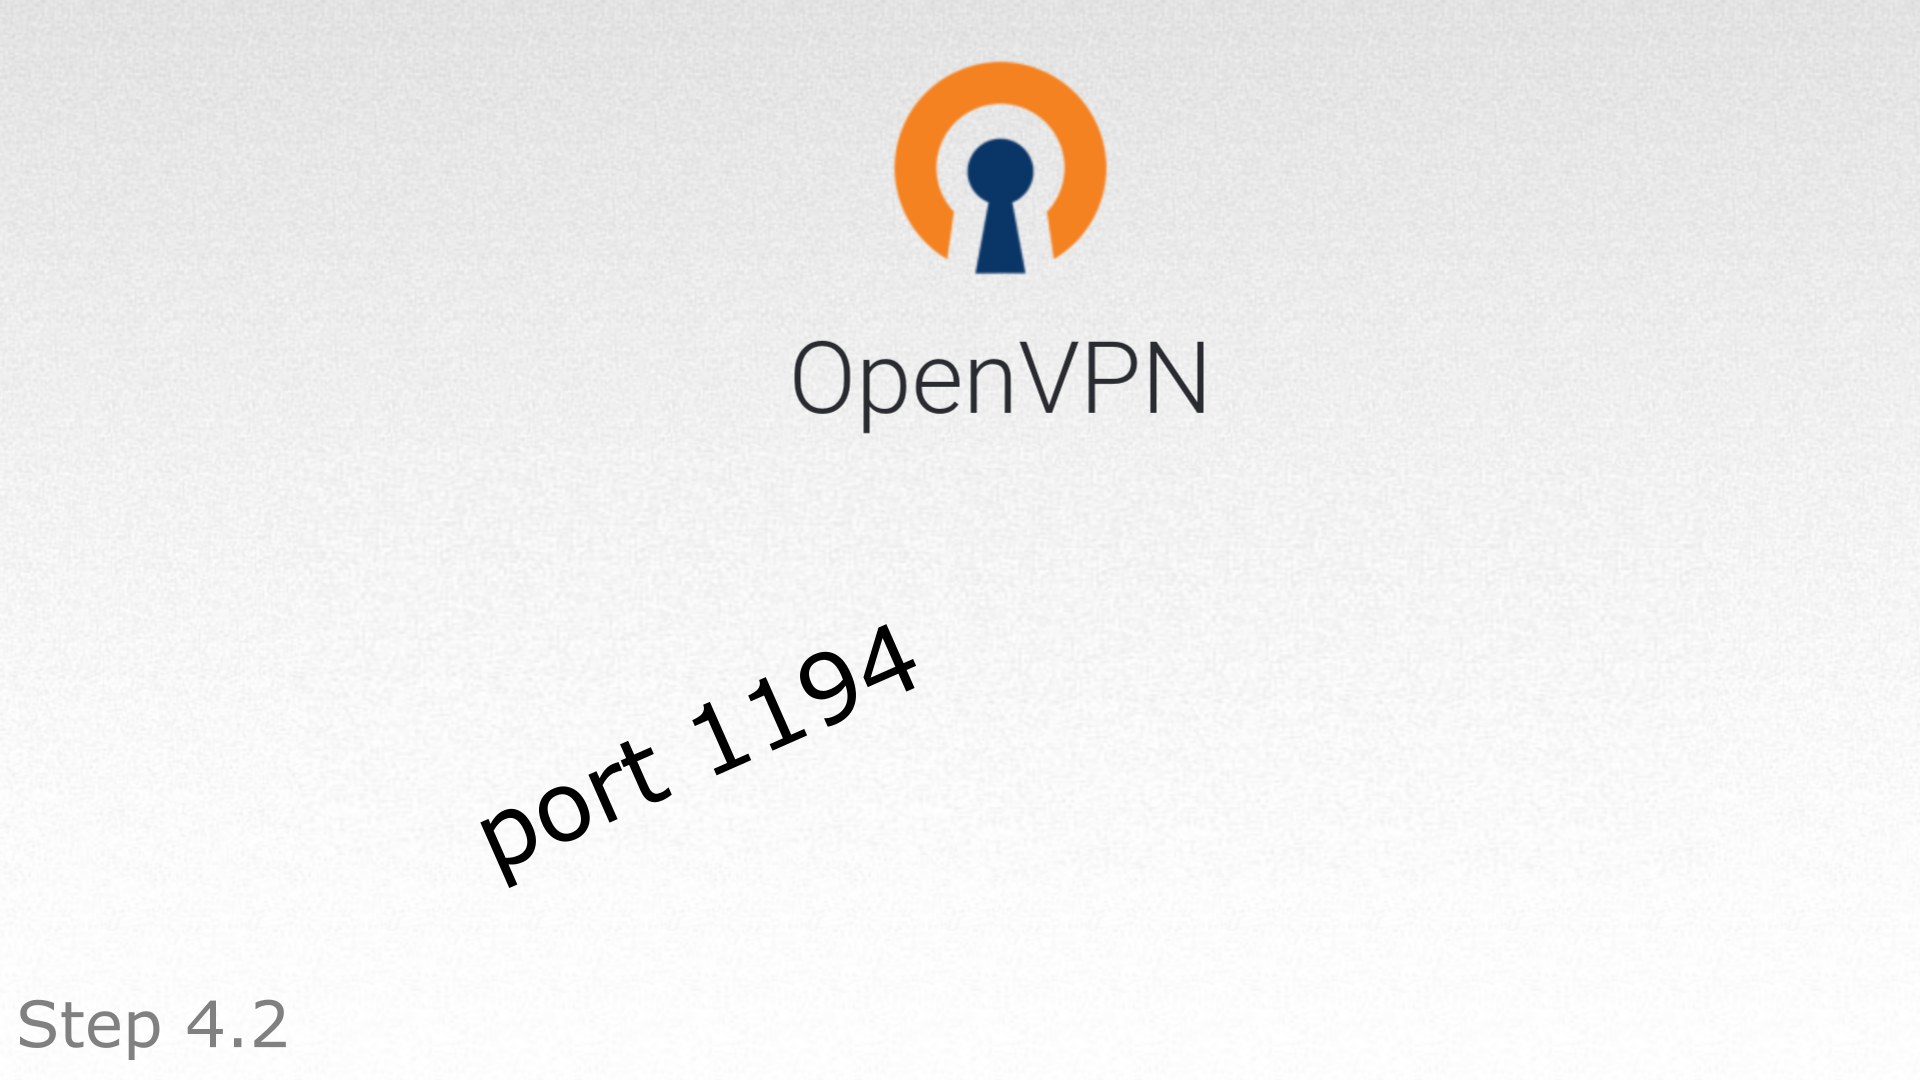
\includegraphics[width=0.7\linewidth]{../frames/53.png}
	\caption{Or the OpenVPN app needs open port 1194. You can find further information in our documentation.}
	\label{fig:40}
\end{figure}

\section{Help}

\begin{figure}[htbp!]
	\centering
	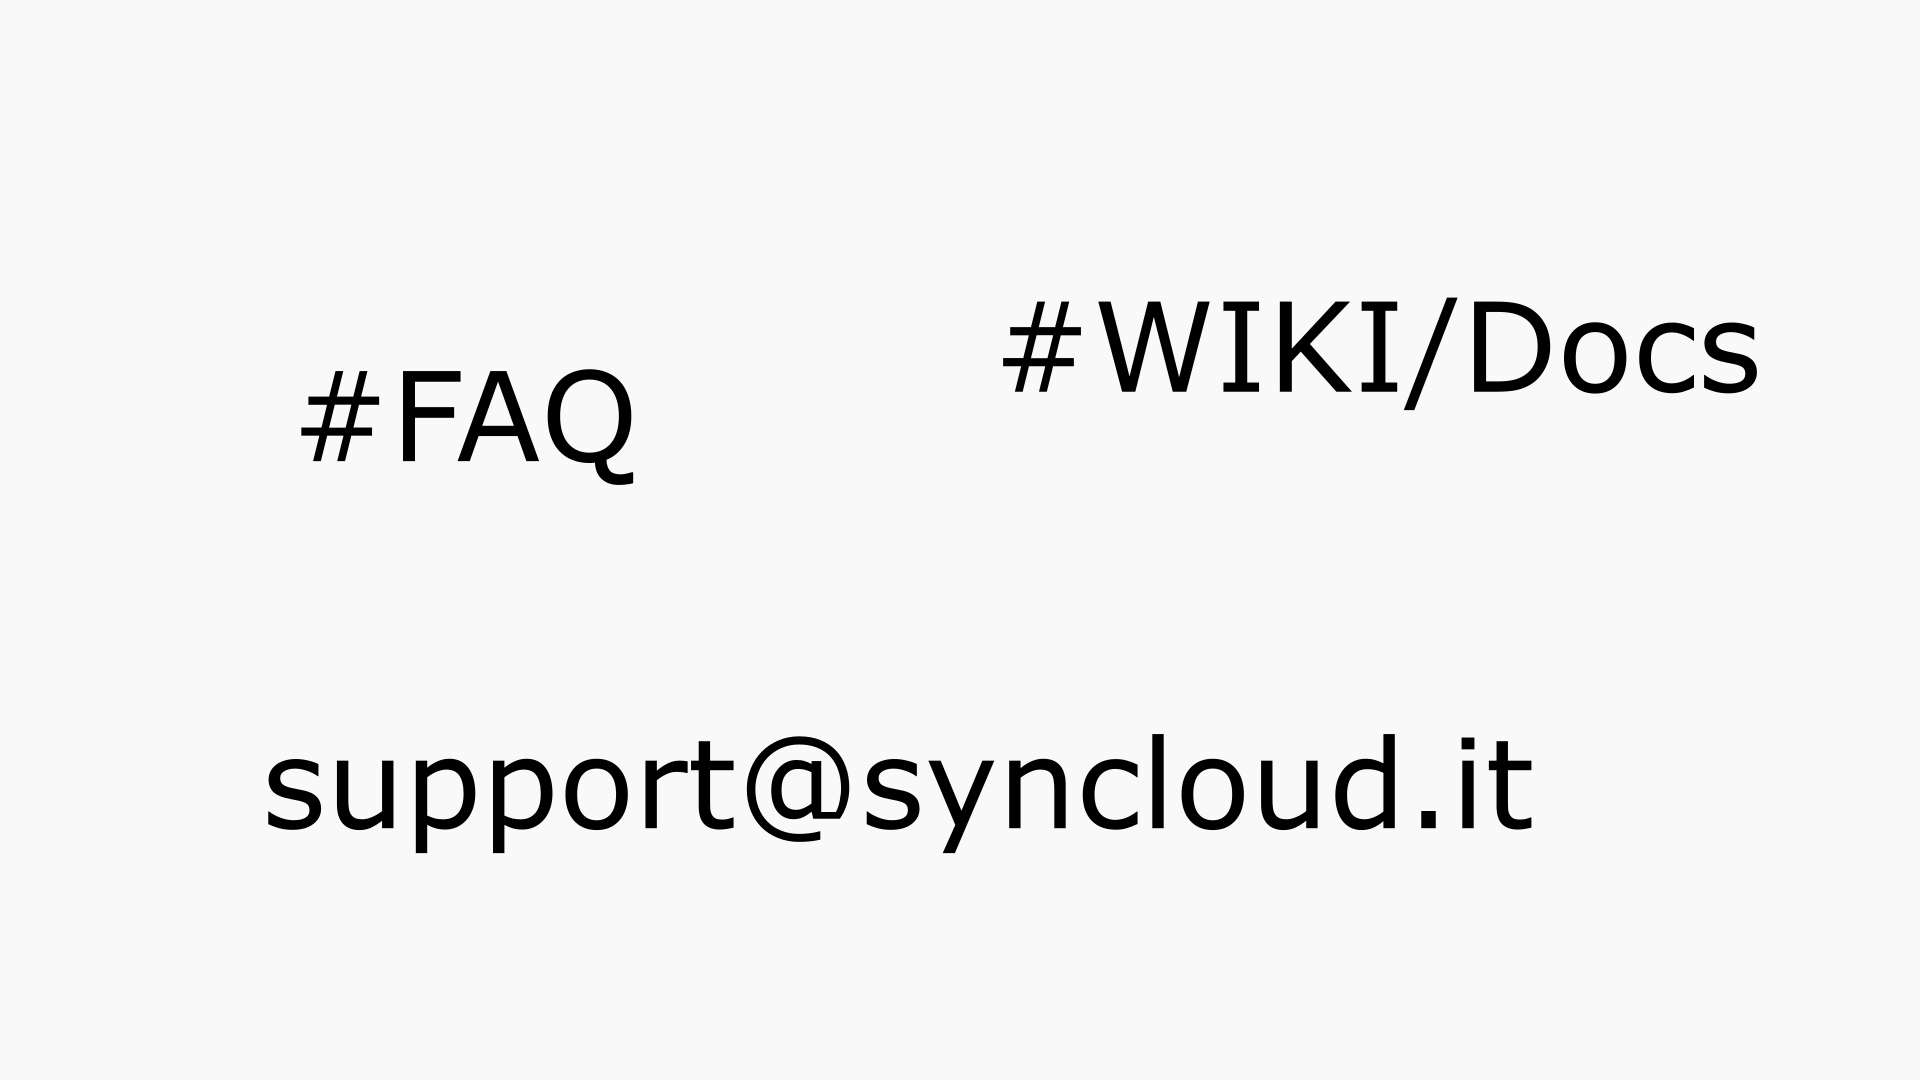
\includegraphics[width=0.7\linewidth]{../frames/56.png}
	\caption{Please visit our FAQs and documentation before contacting our support.}
	\label{fig:41}
\end{figure}

\begin{figure}[htbp!]
	\centering
	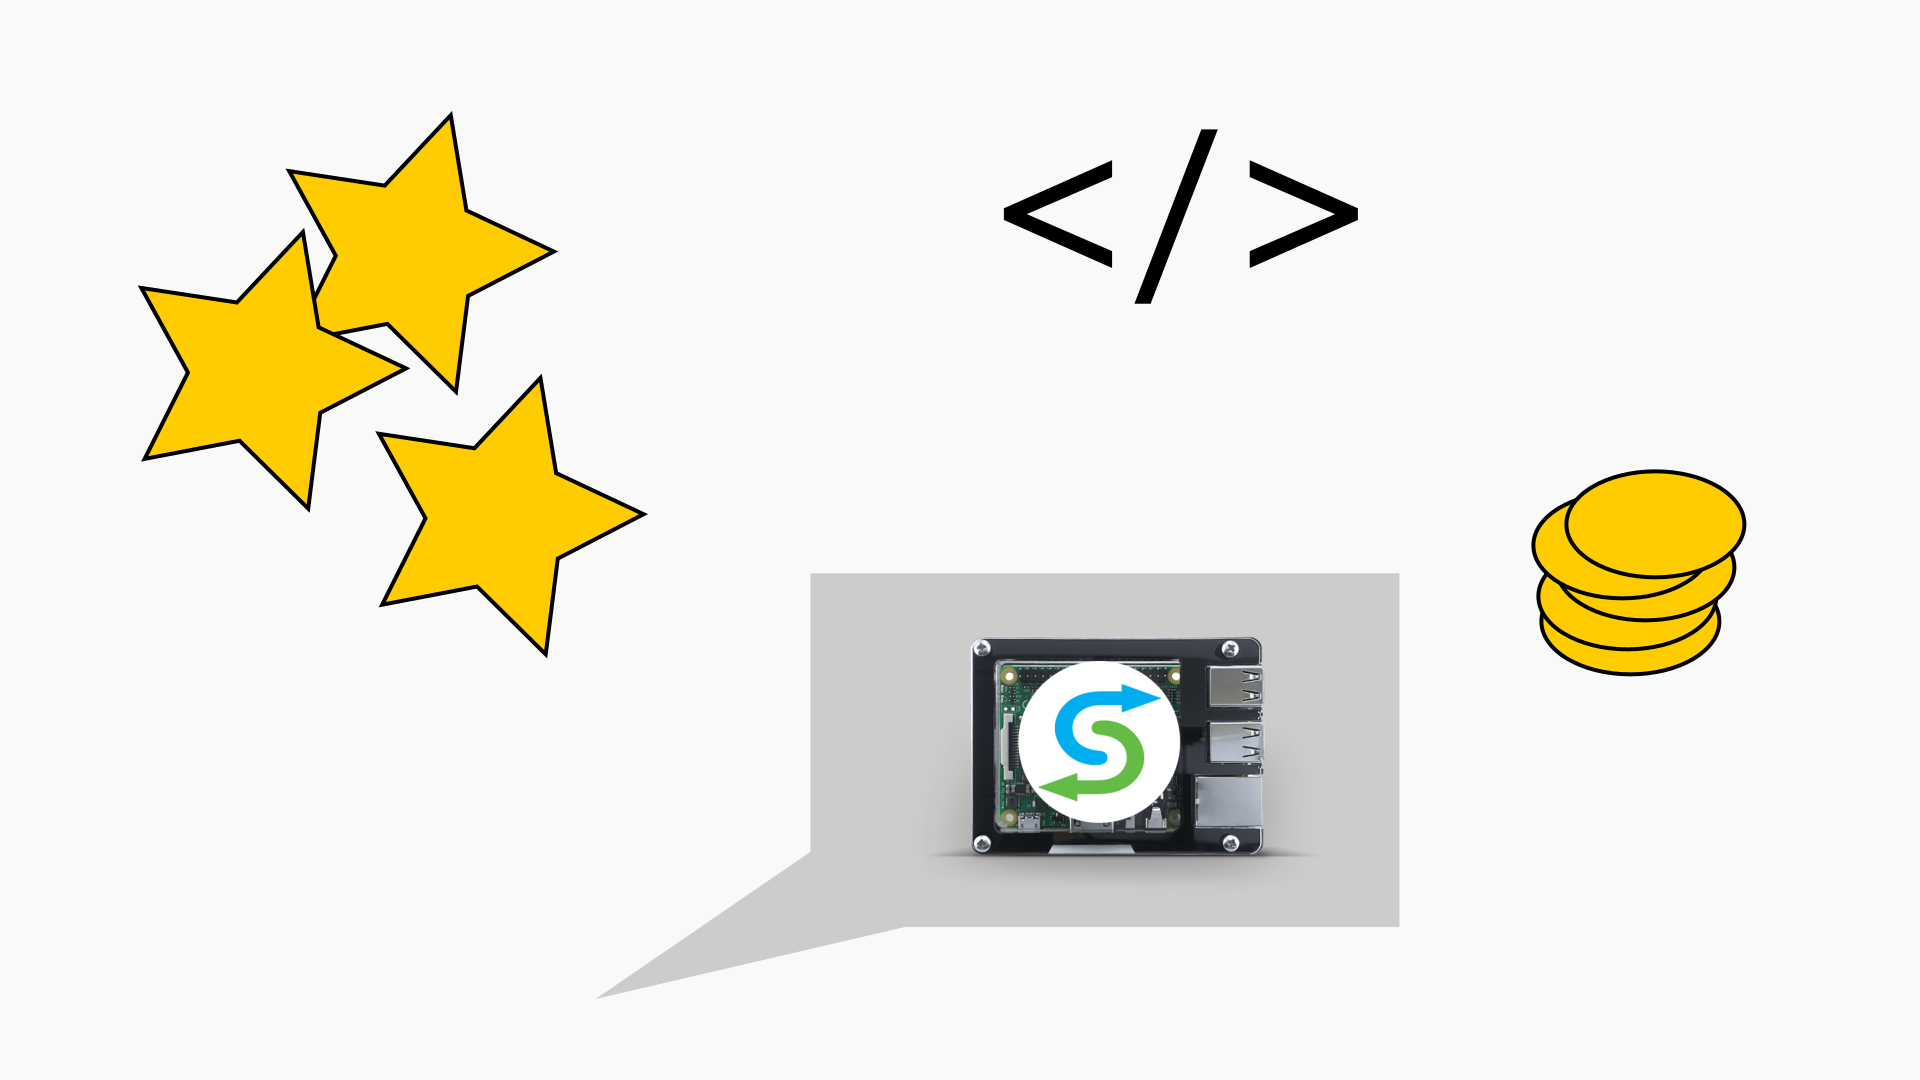
\includegraphics[width=0.7\linewidth]{../frames/60.png}
	\caption{If you like Syncloud, please support us. You can rate our products in the shop, participate on the code on GitHub, donate or buy more products in our shop and tell other persons about Syncloud.}
	\label{fig:42}
\end{figure}

\begin{figure}[htbp!]
	\centering
	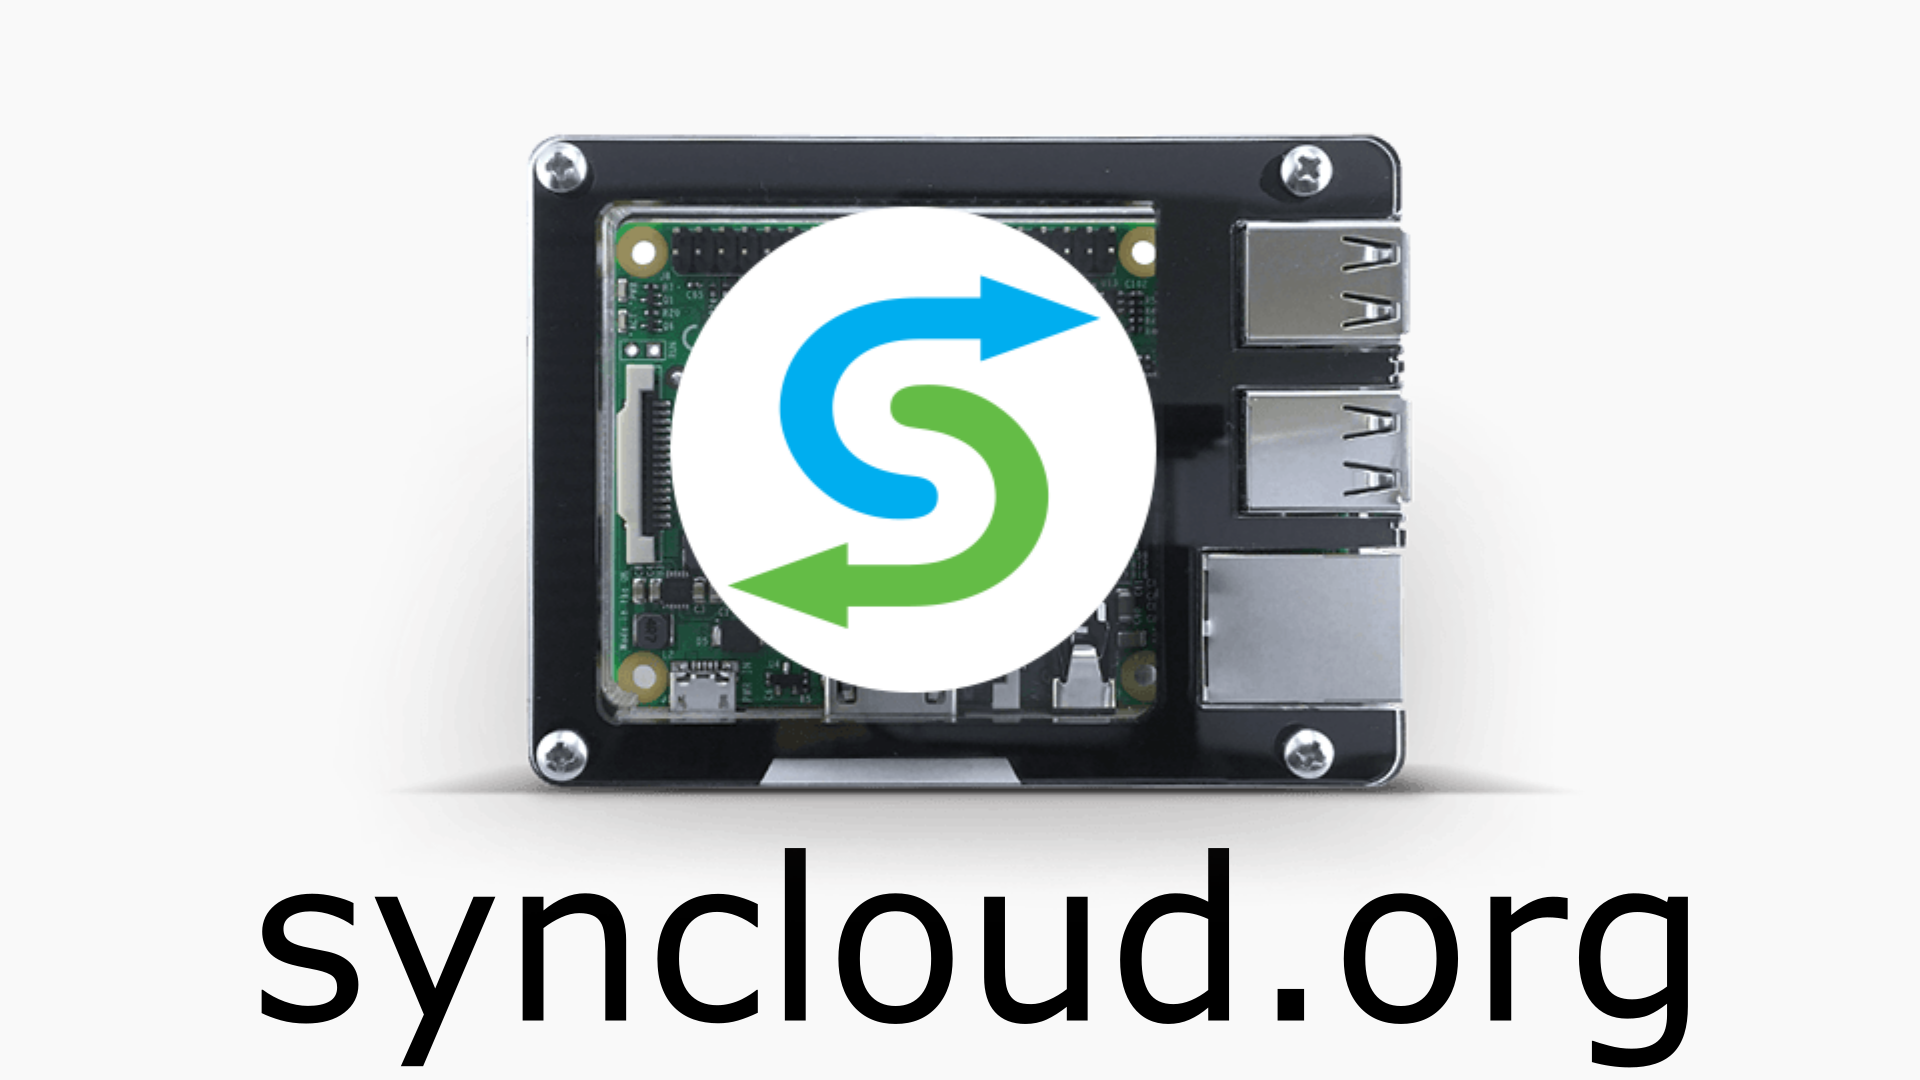
\includegraphics[width=0.7\linewidth]{../frames/61.png}
	\caption{Thanks for watching. Your Syncloud team.}
	\label{fig:43}
\end{figure}

\end{document}
